\documentclass[titlepage=true]{scrartcl}

%%%%%%%%%%%%%%%%%%%%%%%%%%%%%%%%%%%%%%%
%% Makros & anderer Low-Level bastel %%
%%%%%%%%%%%%%%%%%%%%%%%%%%%%%%%%%%%%%%%
\makeatletter
%% Makros für Titel, Autor und Datum 
%% Dank diesem Makro stehen Titel, Autor und Datum überall im Dokument zur verfügung
%% Date hat zudem den Default-Wert \today
\def\@Title{}
\def\@Author{}
\def\@Date{\today}
\newcommand{\Title}{\@Title}
\newcommand{\Author}{\@Author}
\newcommand{\Date}{\@Date}
\AtBeginDocument{%
  \let\@Title\@title
  \let\@Author\@author
  \let\@Date\@date
}

%% Makros für den Arraystretch (bei uns meist in Tabellen genutzt, welche Formeln enthalten)
% Default Value
\def\@ArrayStretchDefault{1} % Entspricht der Voreinstellung von Latex

% Setzt einen neuen Wert für den arraystretch
\newcommand{\setArrayStretch}[1]{\renewcommand{\arraystretch}{#1}}

% Setzt den arraystretch zurück auf den default wert
\newcommand{\resetArrayStretch}{\renewcommand{\arraystretch}{\@ArrayStretchDefault}}

% Makro zum setzten des Default arraystretch. Kann nur in der Präambel verwendet werden.
\newcommand{\setDefaultArrayStretch}[1]{%
	\AtBeginDocument{%
		\def\@ArrayStretchDefault{#1}
		\renewcommand{\arraystretch}{#1}
	}
}
\makeatother


%%%%%%%%%%%%%%%%%%%%%%%
%% Wichtige Packages %%
%%%%%%%%%%%%%%%%%%%%%%%
\usepackage[utf8]{inputenc} % UTF-8 unterstützung
\usepackage[english, ngerman]{babel} % Silbentrennung
%\usepackage[automark]{scrpage2} % Header und Footer
\usepackage[automark]{scrlayer-scrpage} %Ersatz für scrpage2 welches veraltet ist
\usepackage{tabularx}

% Für Abbildungen mit mehreren kleinen Bilder
% Doku: http://www.ctan.org/tex-archive/macros/latex/contrib/caption/
\usepackage[justification=centering]{caption}
\usepackage{subcaption}

\ifx \GUARDhsrColors \undefined
\def\GUARDhsrColors{}

\usepackage[table]{xcolor}

\definecolor{HSRWhite}{cmyk}{0,0,0,0}

\definecolor{HSRBlue}{cmyk}{1,0.4,0,0.2}
\definecolor{HSRBlue80}{cmyk}{0.8,0.32,0,0.16}
\definecolor{HSRBlue60}{cmyk}{0.6,0.24,0,0.12}
\definecolor{HSRBlue40}{cmyk}{0.4,0.16,0,0.08}
\definecolor{HSRBlue20}{cmyk}{0.2,0.08,0,0.04}

\definecolor{HSRLightGray}{cmyk}{0,0,0,0.30}
\definecolor{HSRLightGray80}{cmyk}{0,0,0,0.24}
\definecolor{HSRLightGray60}{cmyk}{0,0,0,0.18}
\definecolor{HSRLightGray40}{cmyk}{0,0,0,0.12}
\definecolor{HSRLightGray20}{cmyk}{0,0,0,0.06}

\definecolor{HSRSchwarz}{cmyk}{0,0,0,1}
\definecolor{HSRSchwarz80}{cmyk}{0,0,0,0.8}
\definecolor{HSRSchwarz60}{cmyk}{0,0,0,0.6}
\definecolor{HSRSchwarz40}{cmyk}{0,0,0,0.4}
\definecolor{HSRSchwarz20}{cmyk}{0,0,0,0.2}

\definecolor{HSRHematite}{cmyk}{0.6,1,0.4,0.2}
\definecolor{HSRHematite80}{cmyk}{0.48,0.80,0.32,0.16}
\definecolor{HSRHematite60}{cmyk}{0.36,0.60,0.24,0.12}
\definecolor{HSRHematite40}{cmyk}{0.24,0.40,0.16,0.08}
\definecolor{HSRHematite20}{cmyk}{0.12,0.20,0.08,0.04}

\definecolor{HSRLakeGreen}{cmyk}{0.70,0.30,0.45,0.05}
\definecolor{HSRLakeGreen80}{cmyk}{0.56,0.24,0.36,0.03}
\definecolor{HSRLakeGreen60}{cmyk}{0.42,0.18,0.27,0.02}
\definecolor{HSRLakeGreen40}{cmyk}{0.28,0.06,0.13,0.06}
\definecolor{HSRLakeGreen20}{cmyk}{0.14,0.06,0.09,0.01}

\definecolor{HSRReed}{cmyk}{0.10,0.25,0.45,0.60}
\definecolor{HSRReed80}{cmyk}{0.08,0.20,0.36,0.48}
\definecolor{HSRReed60}{cmyk}{0.06,0.15,0.27,0.36}
\definecolor{HSRReed40}{cmyk}{0.04,0.10,0.18,0.24}
\definecolor{HSRReed20}{cmyk}{0.02,0.05,0.09,0.12}

\definecolor{HSRPetrol}{cmyk}{1,0.18,0,0.45}
\definecolor{HSRPetrol80}{cmyk}{0.64,0.08,0.12,0.32}
\definecolor{HSRPetrol60}{cmyk}{0.48,0.06,0.09,0.24}
\definecolor{HSRPetrol40}{cmyk}{0.32,0.04,0.06,0.16}
\definecolor{HSRPetrol20}{cmyk}{0.16,0.02,0.03,0.08}

\definecolor{HSRBasswood}{cmyk}{0.25,0.05,0.70,0.15}
\definecolor{HSRBasswood80}{cmyk}{0.20,0.04,0.56,0.12}
\definecolor{HSRBasswood60}{cmyk}{0.15,0.03,0.42,0.09}
\definecolor{HSRBasswood40}{cmyk}{0.10,0.02,0.28,0.06}
\definecolor{HSRBasswood20}{cmyk}{0.05,0.01,0.14,0.03}


\fi
\ifx\GUARDmathe\undefined
\def\GUARDmathe{}

\usepackage{amssymb}
% Das mathtools package ist eine Erweiterung zum amsmath package.
% Das amsmath package wird dabei automatisch geladen
\usepackage{mathtools}


% Package mit vielen weiteren Mathe Symbolen
% http://www.ctan.org/tex-archive/fonts/mathabx
\usepackage{mathabx}

% This package defines commands to access bold math symbols. The basic command
% is \bm which may be used to make the math expression in its argument be typeset
% using bold fonts.
\usepackage{bm}

% Package for differentiation operators
\usepackage{esdiff}

\fi
\ifx\GUARDenumitem\undefined
\def\GUARDenumitem{}

\usepackage{enumitem}
\setitemize{noitemsep,topsep=0pt,parsep=0pt,partopsep=0pt}
\setenumerate{noitemsep,topsep=0pt,parsep=0pt,partopsep=0pt}
\fi
\ifx\GUARDlistings\undefined
\def\GUARDlistings{}

%TODO Auf HSR-Farben ändern 
\definecolor{mygreen}{rgb}{0,0.6,0}
\definecolor{mygray}{rgb}{0.5,0.5,0.5}
\definecolor{mymauve}{rgb}{0.58,0,0.82}

\usepackage{listings}
\lstset{ %
    firstnumber=1,
    backgroundcolor=\color{white},   % choose the background color; you must add        \usepackage{color} or \usepackage{xcolor}
    basicstyle=\footnotesize\ttfamily, % the size of the fonts that are used for the code
    breakatwhitespace=false,         % sets if automatic breaks should only happen at whitespace
    breaklines=true,                 % sets automatic line breaking
    captionpos=b,                    % sets the caption-position to bottom
    commentstyle=\color{mygreen},    % comment style
    deletekeywords={...},            % if you want to delete keywords from the given language
    otherkeywords={...},             % if you want to add more keywords to the set
    escapeinside={\%*}{*\%},          % if you want to add LaTeX within your code
    extendedchars=true,              % lets you use non-ASCII characters; for 8-bits encodings only, does not work with UTF-8
    frame=single,	                 % adds a frame around the code
    keepspaces=true,                 % keeps spaces in text, useful for keeping indentation of code (possibly needs columns=flexible)
    keywordstyle=\color{blue},       % keyword style
    language=C++,                    % the language of the code   
    numbers=left,                    % where to put the line-numbers; possible values are (none, left, right)
    numbersep=5pt,                   % how far the line-numbers are from the code
    numberstyle=\tiny\color{mygray}, % the style that is used for the line-numbers
    rulecolor=\color{black},         % if not set, the frame-color may be changed on line-breaks within not-black text (e.g. comments (green here))
    showspaces=false,                % show spaces everywhere adding particular underscores; it overrides 'showstringspaces'
    showstringspaces=false,          % underline spaces within strings only
    showtabs=false,                  % show tabs within strings adding particular underscores
    stepnumber=2,                    % the step between two line-numbers. If it's 1, each line will be numbered
    stringstyle=\color{mymauve},     % string literal style
    tabsize=2,	                     % sets default tabsize to 2 spaces
    %title=\lstname                   % show the filename of files included with         \lstinputlisting; also try caption instead of title
}

\lstdefinestyle{Java}{ numbers=left,
  belowcaptionskip=1\baselineskip,
  breaklines=true,
  frame=L,
  xleftmargin=10pt,
  language=Java,
  showstringspaces=false,
  basicstyle=\footnotesize\ttfamily,
  keywordstyle=\bfseries\color{green!40!black},
  commentstyle=\itshape\color{purple!40!black},
  identifierstyle=\color{blue},
  stringstyle=\color{orange},
  numberstyle=\ttfamily\tiny,
  tabsize=2
}

\lstdefinestyle{SQL}{
  numbers=none,
  belowcaptionskip=1\baselineskip,
  breaklines=true,
  xleftmargin=10pt,
  language=SQL,
  showstringspaces=false,
  basicstyle=\footnotesize\ttfamily,
  keywordstyle=\bfseries\color{green!40!black},
  commentstyle=\itshape\color{purple!40!black},
  identifierstyle=\color{blue},
  stringstyle=\color{orange},,
  tabsize=2
}

\lstdefinestyle{C}{
  numbers=left,
  belowcaptionskip=1\baselineskip,
  breaklines=true,
  frame=L,
  xleftmargin=10pt,
  language=C,
  showstringspaces=false,
  basicstyle=\footnotesize\ttfamily,
  keywordstyle=\bfseries\color{green!40!black},
  commentstyle=\itshape\color{purple!40!black},
  identifierstyle=\color{blue},
  stringstyle=\color{orange},
  numberstyle=\ttfamily\tiny,
  tabsize=2
}

\lstdefinestyle{Cpp}{
  numbers=left,
  belowcaptionskip=1\baselineskip,
  breaklines=true,
  frame=L,
  xleftmargin=10pt,
  language=C++,
  showstringspaces=false,
  basicstyle=\footnotesize\ttfamily,
  keywordstyle=\bfseries\color{green!40!black},
  commentstyle=\itshape\color{purple!40!black},
  identifierstyle=\color{blue},
  stringstyle=\color{orange},
  numberstyle=\ttfamily\tiny,
  tabsize=2
}

\lstdefinestyle{Cppunit}{
    belowcaptionskip=1\baselineskip,
    %frame=L,
    xleftmargin=\parindent,
    language=C++,
    keywordstyle=\bfseries\color{blue},
    keywordstyle=[2]\bf\color{black}, %not sure why \bf works, but it does
    commentstyle=\itshape\color{mygreen},
    identifierstyle=\color{black},
    stringstyle=\color{gray},
    keywords=[2]{  %Cpp Unit Keywords
        CPPUNIT_ASSERT,
        CPPUNIT_TEST,
        CPPUNIT_TEST_EXCEPTION,
        CPPUNIT_TEST_END,
        CPPUNIT_TEST_SUITE,
        CPPUNIT_TEST_SUITE_REGISTRATION,
        CPPUNIT_TEST_SUITE_END},
}

\lstdefinestyle{CppQT}{
    belowcaptionskip=1\baselineskip,
    %frame=L,
    xleftmargin=\parindent,
    language=C++,
    keywordstyle=\bfseries\color{blue},
    keywordstyle=[2]\bfseries\color{red},
    commentstyle=\itshape\color{mygreen},
    identifierstyle=\color{black},
    stringstyle=\color{gray},
    keywords=[2]{           % qt-Keywords
        Qt,
        SIGNAL,
        SLOT,
        QApplication,
        QDialog,
        QGridLayout,
        QPushButton,
        QLabel,
        QVBoxLayout,
        QHBoxLayout,
        QWidget,
        QGroupBox,
        QFont,
        QLineEdit,
        QRadioButton,
        QPen,
        QRect,
        QPaintEvent,
        QBrush,
        QPixmap,
        QPainter,
        QString,
        QPoint,
        update()},
}

\lstdefinestyle{Cdoxy}{
    belowcaptionskip=1\baselineskip,
    %frame=L,
    xleftmargin=\parindent,
    language=C++,  
    keywordstyle=\bfseries\color{blue},
    commentstyle=\itshape\color{mygreen},
    identifierstyle=\color{black},
    stringstyle=\color{gray},
    otherkeywords={           % DoxygenKeywords
        ...,
        ....,
        @mainpage,
        @file,
        @author,
        @version,
        @date,
        @bug,
        @brief,
        @extended,
        @param,
        @return,
        @warning,
        @note,
        @see},
}

\lstdefinestyle{Csharp}{
  numbers=left,
  belowcaptionskip=1\baselineskip,
  breaklines=true,
  frame=L,
  xleftmargin=10pt,
  language=[Sharp]C,
  showstringspaces=false,
  basicstyle=\footnotesize\ttfamily,
  keywordstyle=\bfseries\color{green!40!black},
  commentstyle=\itshape\color{purple!40!black},
  identifierstyle=\color{blue},
  stringstyle=\color{orange},
  numberstyle=\ttfamily\tiny,
  tabsize=2
}

\lstdefinestyle{Matlab}{
  numbers=left,
  belowcaptionskip=1\baselineskip,
  breaklines=true,
  frame=L,
  xleftmargin=10pt,
  language=Matlab,
  showstringspaces=false,
  basicstyle=\footnotesize\ttfamily,
  keywordstyle=\bfseries\color{blue},
  commentstyle=\itshape\color{mygreen},
  identifierstyle=\color{black},
  stringstyle=\color{orange},
  numberstyle=\ttfamily\tiny,
  tabsize=2,
  otherkeywords={
      solve,
      int,
      double,
      syms,
      interp1}
}

\lstdefinestyle{VHDL}{
  numbers=left,
  belowcaptionskip=1\baselineskip,
  breaklines=true,
  frame=L,
  xleftmargin=0pt,
  language=VHDL,
  showstringspaces=false,
  basicstyle=\footnotesize\ttfamily,
  keywordstyle=\bfseries\color{green!40!black},
  commentstyle=\itshape\color{purple!40!black},
  identifierstyle=\color{blue},
  stringstyle=\color{orange},
  numberstyle=\ttfamily\tiny,
  tabsize=2
}

\lstdefinestyle{ASM}{
  numbers=left,
  belowcaptionskip=1\baselineskip,
  breaklines=true,
  frame=L,
  xleftmargin=10pt,
  language=[x86masm]Assembler,
  showstringspaces=false,
  basicstyle=\footnotesize\ttfamily,
  keywordstyle=\bfseries\color{green!40!black},
  commentstyle=\itshape\color{purple!40!black},
  identifierstyle=\color{blue},
  stringstyle=\color{orange},
  numberstyle=\ttfamily\tiny,
  tabsize=2
}

\lstdefinestyle{R}{
  numbers=left,
  belowcaptionskip=1\baselineskip,
  breaklines=true,
  frame=L,
  xleftmargin=10pt,
  aboveskip=-5pt,
  language=R,
  showstringspaces=false,
  basicstyle=\footnotesize\ttfamily,
  keywordstyle=\bfseries\color{green!40!black},
  commentstyle=\itshape\color{purple!40!black},
  identifierstyle=\color{blue},
  stringstyle=\color{orange},
  numberstyle=\ttfamily\tiny,
  tabsize=1
}
\fi


% Seitenränder für Formelsammlungen 
\usepackage[left=1cm,right=1cm,top=0.5cm,bottom=0.5cm,includeheadfoot]{geometry}

\usepackage[plainpages=false,pdfpagelabels]{hyperref}
\hypersetup{
	pdfstartview={FitH}, % fits the width of the page to the window
	pdfauthor={\Author},
	pdfcreator={\Author},
	pdfproducer={\Author},
	pdftitle={\Title},
	colorlinks=true,
	linkcolor=HSRBlue,
	citecolor=HSRReed,
	filecolor=HSRLake,
	urlcolor=HSRHematite
}

\usepackage{longtable}
\usepackage[europeanresistors,americaninductors]{circuitikz}
\usepackage{multirow} % Create tabular cells spanning multiple rows
\usepackage{multicol} % In­ter­mix sin­gle and mul­ti­ple columns
\usepackage{rotating} % Rotation tools, including rotated fullpage floats


%%%%%%%%%%%%%%%%%%%%%%%%%%%%%%%%%%%
%% Layout der Kopf und Fusszeile %%
%%%%%%%%%%%%%%%%%%%%%%%%%%%%%%%%%%%
\deftriplepagestyle{zusammenfassung}[0pt][0.5pt]
{\Title}	% Kopfzeile innen
{\headmark}	% Kopfzeile mitte
{\pagemark}	% Kopfzeile aussen
{\Author}	% Fusszeile innen
{}			% Fusszeile mitte
{\Date}	% Fusszeile aussen
\pagestyle{zusammenfassung}

% Nummerierte und unnummerierte paragraph headings
\setcounter{secnumdepth}{5}

\RedeclareSectionCommands[
	afterskip=1em
]{paragraph,subparagraph}

\renewcommand*{\paragraphformat}{\theparagraph\autodot\enskip}
\renewcommand*{\subparagraphformat}{\thesubparagraph\autodot\enskip}


%%Makros%%%%%%%%%%%%%%%%%%%%%%%%%%%%%%%%%%%%%%%%%%%  
% Command for images in table
\newcommand\tabImg[2][]{%
	\raisebox{0pt}[\dimexpr\totalheight+\dp\strutbox\relax][\dp\strutbox]{%
		\includegraphics[#1]{#2}%
	}%
}

% Makros für Verweise auf ein Buch oder Skript
\newcommand{\buch}[1]{\texorpdfstring{$_{\textcolor{HSRLakeGreen}{\mbox{\small{#1}}}}$}{}}
\newcommand{\buchSeite}[1]{\texorpdfstring{\ensuremath{_{\textcolor{red}{\mbox{\small{ S#1}}}}}}{}}
\newcommand{\skript}[1]{\texorpdfstring{$_{\textcolor{HSRReed}{\mbox{\small{#1}}}}$}{}}
\newcommand{\formelbuch}[1]{$_{\textcolor{red}{\mbox{\small{S#1}}}}$}

% Zeilenhöhe Tabellen:
\newcommand{\arraystretchOriginal}{1.5}
\renewcommand{\arraystretch}{\arraystretchOriginal}

\setlength{\parindent}{0pt}

% Todo command
\newcommand{\todo}[1]{\textbf{\color{red}{TO DO: #1}}}
% \ifx\GUARDhyperref\undefined
\def\GUARDhyperref{}

\ifx \GUARDhsrColors \undefined
\def\GUARDhsrColors{}

\usepackage[table]{xcolor}

\definecolor{HSRWhite}{cmyk}{0,0,0,0}

\definecolor{HSRBlue}{cmyk}{1,0.4,0,0.2}
\definecolor{HSRBlue80}{cmyk}{0.8,0.32,0,0.16}
\definecolor{HSRBlue60}{cmyk}{0.6,0.24,0,0.12}
\definecolor{HSRBlue40}{cmyk}{0.4,0.16,0,0.08}
\definecolor{HSRBlue20}{cmyk}{0.2,0.08,0,0.04}

\definecolor{HSRLightGray}{cmyk}{0,0,0,0.30}
\definecolor{HSRLightGray80}{cmyk}{0,0,0,0.24}
\definecolor{HSRLightGray60}{cmyk}{0,0,0,0.18}
\definecolor{HSRLightGray40}{cmyk}{0,0,0,0.12}
\definecolor{HSRLightGray20}{cmyk}{0,0,0,0.06}

\definecolor{HSRSchwarz}{cmyk}{0,0,0,1}
\definecolor{HSRSchwarz80}{cmyk}{0,0,0,0.8}
\definecolor{HSRSchwarz60}{cmyk}{0,0,0,0.6}
\definecolor{HSRSchwarz40}{cmyk}{0,0,0,0.4}
\definecolor{HSRSchwarz20}{cmyk}{0,0,0,0.2}

\definecolor{HSRHematite}{cmyk}{0.6,1,0.4,0.2}
\definecolor{HSRHematite80}{cmyk}{0.48,0.80,0.32,0.16}
\definecolor{HSRHematite60}{cmyk}{0.36,0.60,0.24,0.12}
\definecolor{HSRHematite40}{cmyk}{0.24,0.40,0.16,0.08}
\definecolor{HSRHematite20}{cmyk}{0.12,0.20,0.08,0.04}

\definecolor{HSRLakeGreen}{cmyk}{0.70,0.30,0.45,0.05}
\definecolor{HSRLakeGreen80}{cmyk}{0.56,0.24,0.36,0.03}
\definecolor{HSRLakeGreen60}{cmyk}{0.42,0.18,0.27,0.02}
\definecolor{HSRLakeGreen40}{cmyk}{0.28,0.06,0.13,0.06}
\definecolor{HSRLakeGreen20}{cmyk}{0.14,0.06,0.09,0.01}

\definecolor{HSRReed}{cmyk}{0.10,0.25,0.45,0.60}
\definecolor{HSRReed80}{cmyk}{0.08,0.20,0.36,0.48}
\definecolor{HSRReed60}{cmyk}{0.06,0.15,0.27,0.36}
\definecolor{HSRReed40}{cmyk}{0.04,0.10,0.18,0.24}
\definecolor{HSRReed20}{cmyk}{0.02,0.05,0.09,0.12}

\definecolor{HSRPetrol}{cmyk}{1,0.18,0,0.45}
\definecolor{HSRPetrol80}{cmyk}{0.64,0.08,0.12,0.32}
\definecolor{HSRPetrol60}{cmyk}{0.48,0.06,0.09,0.24}
\definecolor{HSRPetrol40}{cmyk}{0.32,0.04,0.06,0.16}
\definecolor{HSRPetrol20}{cmyk}{0.16,0.02,0.03,0.08}

\definecolor{HSRBasswood}{cmyk}{0.25,0.05,0.70,0.15}
\definecolor{HSRBasswood80}{cmyk}{0.20,0.04,0.56,0.12}
\definecolor{HSRBasswood60}{cmyk}{0.15,0.03,0.42,0.09}
\definecolor{HSRBasswood40}{cmyk}{0.10,0.02,0.28,0.06}
\definecolor{HSRBasswood20}{cmyk}{0.05,0.01,0.14,0.03}


\fi

\usepackage[plainpages=false,pdfpagelabels]{hyperref}
\hypersetup{
  pdfstartview={FitH}, % fits the width of the page to the window
  pdfauthor={\Author},
  pdfcreator={\Author},
  pdfproducer={\Author},
  pdftitle={\Title},
  colorlinks=true,
  linkcolor=HSRBlue,
  citecolor=HSRReed,
  filecolor=HSRLake,
  urlcolor=HSRHematite
}

\fi

\ifx\GUARDlistings\undefined
\def\GUARDlistings{}

%TODO Auf HSR-Farben ändern 
\definecolor{mygreen}{rgb}{0,0.6,0}
\definecolor{mygray}{rgb}{0.5,0.5,0.5}
\definecolor{mymauve}{rgb}{0.58,0,0.82}

\usepackage{listings}
\lstset{ %
    firstnumber=1,
    backgroundcolor=\color{white},   % choose the background color; you must add        \usepackage{color} or \usepackage{xcolor}
    basicstyle=\footnotesize\ttfamily, % the size of the fonts that are used for the code
    breakatwhitespace=false,         % sets if automatic breaks should only happen at whitespace
    breaklines=true,                 % sets automatic line breaking
    captionpos=b,                    % sets the caption-position to bottom
    commentstyle=\color{mygreen},    % comment style
    deletekeywords={...},            % if you want to delete keywords from the given language
    otherkeywords={...},             % if you want to add more keywords to the set
    escapeinside={\%*}{*\%},          % if you want to add LaTeX within your code
    extendedchars=true,              % lets you use non-ASCII characters; for 8-bits encodings only, does not work with UTF-8
    frame=single,	                 % adds a frame around the code
    keepspaces=true,                 % keeps spaces in text, useful for keeping indentation of code (possibly needs columns=flexible)
    keywordstyle=\color{blue},       % keyword style
    language=C++,                    % the language of the code   
    numbers=left,                    % where to put the line-numbers; possible values are (none, left, right)
    numbersep=5pt,                   % how far the line-numbers are from the code
    numberstyle=\tiny\color{mygray}, % the style that is used for the line-numbers
    rulecolor=\color{black},         % if not set, the frame-color may be changed on line-breaks within not-black text (e.g. comments (green here))
    showspaces=false,                % show spaces everywhere adding particular underscores; it overrides 'showstringspaces'
    showstringspaces=false,          % underline spaces within strings only
    showtabs=false,                  % show tabs within strings adding particular underscores
    stepnumber=2,                    % the step between two line-numbers. If it's 1, each line will be numbered
    stringstyle=\color{mymauve},     % string literal style
    tabsize=2,	                     % sets default tabsize to 2 spaces
    %title=\lstname                   % show the filename of files included with         \lstinputlisting; also try caption instead of title
}

\lstdefinestyle{Java}{ numbers=left,
  belowcaptionskip=1\baselineskip,
  breaklines=true,
  frame=L,
  xleftmargin=10pt,
  language=Java,
  showstringspaces=false,
  basicstyle=\footnotesize\ttfamily,
  keywordstyle=\bfseries\color{green!40!black},
  commentstyle=\itshape\color{purple!40!black},
  identifierstyle=\color{blue},
  stringstyle=\color{orange},
  numberstyle=\ttfamily\tiny,
  tabsize=2
}

\lstdefinestyle{SQL}{
  numbers=none,
  belowcaptionskip=1\baselineskip,
  breaklines=true,
  xleftmargin=10pt,
  language=SQL,
  showstringspaces=false,
  basicstyle=\footnotesize\ttfamily,
  keywordstyle=\bfseries\color{green!40!black},
  commentstyle=\itshape\color{purple!40!black},
  identifierstyle=\color{blue},
  stringstyle=\color{orange},,
  tabsize=2
}

\lstdefinestyle{C}{
  numbers=left,
  belowcaptionskip=1\baselineskip,
  breaklines=true,
  frame=L,
  xleftmargin=10pt,
  language=C,
  showstringspaces=false,
  basicstyle=\footnotesize\ttfamily,
  keywordstyle=\bfseries\color{green!40!black},
  commentstyle=\itshape\color{purple!40!black},
  identifierstyle=\color{blue},
  stringstyle=\color{orange},
  numberstyle=\ttfamily\tiny,
  tabsize=2
}

\lstdefinestyle{Cpp}{
  numbers=left,
  belowcaptionskip=1\baselineskip,
  breaklines=true,
  frame=L,
  xleftmargin=10pt,
  language=C++,
  showstringspaces=false,
  basicstyle=\footnotesize\ttfamily,
  keywordstyle=\bfseries\color{green!40!black},
  commentstyle=\itshape\color{purple!40!black},
  identifierstyle=\color{blue},
  stringstyle=\color{orange},
  numberstyle=\ttfamily\tiny,
  tabsize=2
}

\lstdefinestyle{Cppunit}{
    belowcaptionskip=1\baselineskip,
    %frame=L,
    xleftmargin=\parindent,
    language=C++,
    keywordstyle=\bfseries\color{blue},
    keywordstyle=[2]\bf\color{black}, %not sure why \bf works, but it does
    commentstyle=\itshape\color{mygreen},
    identifierstyle=\color{black},
    stringstyle=\color{gray},
    keywords=[2]{  %Cpp Unit Keywords
        CPPUNIT_ASSERT,
        CPPUNIT_TEST,
        CPPUNIT_TEST_EXCEPTION,
        CPPUNIT_TEST_END,
        CPPUNIT_TEST_SUITE,
        CPPUNIT_TEST_SUITE_REGISTRATION,
        CPPUNIT_TEST_SUITE_END},
}

\lstdefinestyle{CppQT}{
    belowcaptionskip=1\baselineskip,
    %frame=L,
    xleftmargin=\parindent,
    language=C++,
    keywordstyle=\bfseries\color{blue},
    keywordstyle=[2]\bfseries\color{red},
    commentstyle=\itshape\color{mygreen},
    identifierstyle=\color{black},
    stringstyle=\color{gray},
    keywords=[2]{           % qt-Keywords
        Qt,
        SIGNAL,
        SLOT,
        QApplication,
        QDialog,
        QGridLayout,
        QPushButton,
        QLabel,
        QVBoxLayout,
        QHBoxLayout,
        QWidget,
        QGroupBox,
        QFont,
        QLineEdit,
        QRadioButton,
        QPen,
        QRect,
        QPaintEvent,
        QBrush,
        QPixmap,
        QPainter,
        QString,
        QPoint,
        update()},
}

\lstdefinestyle{Cdoxy}{
    belowcaptionskip=1\baselineskip,
    %frame=L,
    xleftmargin=\parindent,
    language=C++,  
    keywordstyle=\bfseries\color{blue},
    commentstyle=\itshape\color{mygreen},
    identifierstyle=\color{black},
    stringstyle=\color{gray},
    otherkeywords={           % DoxygenKeywords
        ...,
        ....,
        @mainpage,
        @file,
        @author,
        @version,
        @date,
        @bug,
        @brief,
        @extended,
        @param,
        @return,
        @warning,
        @note,
        @see},
}

\lstdefinestyle{Csharp}{
  numbers=left,
  belowcaptionskip=1\baselineskip,
  breaklines=true,
  frame=L,
  xleftmargin=10pt,
  language=[Sharp]C,
  showstringspaces=false,
  basicstyle=\footnotesize\ttfamily,
  keywordstyle=\bfseries\color{green!40!black},
  commentstyle=\itshape\color{purple!40!black},
  identifierstyle=\color{blue},
  stringstyle=\color{orange},
  numberstyle=\ttfamily\tiny,
  tabsize=2
}

\lstdefinestyle{Matlab}{
  numbers=left,
  belowcaptionskip=1\baselineskip,
  breaklines=true,
  frame=L,
  xleftmargin=10pt,
  language=Matlab,
  showstringspaces=false,
  basicstyle=\footnotesize\ttfamily,
  keywordstyle=\bfseries\color{blue},
  commentstyle=\itshape\color{mygreen},
  identifierstyle=\color{black},
  stringstyle=\color{orange},
  numberstyle=\ttfamily\tiny,
  tabsize=2,
  otherkeywords={
      solve,
      int,
      double,
      syms,
      interp1}
}

\lstdefinestyle{VHDL}{
  numbers=left,
  belowcaptionskip=1\baselineskip,
  breaklines=true,
  frame=L,
  xleftmargin=0pt,
  language=VHDL,
  showstringspaces=false,
  basicstyle=\footnotesize\ttfamily,
  keywordstyle=\bfseries\color{green!40!black},
  commentstyle=\itshape\color{purple!40!black},
  identifierstyle=\color{blue},
  stringstyle=\color{orange},
  numberstyle=\ttfamily\tiny,
  tabsize=2
}

\lstdefinestyle{ASM}{
  numbers=left,
  belowcaptionskip=1\baselineskip,
  breaklines=true,
  frame=L,
  xleftmargin=10pt,
  language=[x86masm]Assembler,
  showstringspaces=false,
  basicstyle=\footnotesize\ttfamily,
  keywordstyle=\bfseries\color{green!40!black},
  commentstyle=\itshape\color{purple!40!black},
  identifierstyle=\color{blue},
  stringstyle=\color{orange},
  numberstyle=\ttfamily\tiny,
  tabsize=2
}

\lstdefinestyle{R}{
  numbers=left,
  belowcaptionskip=1\baselineskip,
  breaklines=true,
  frame=L,
  xleftmargin=10pt,
  aboveskip=-5pt,
  language=R,
  showstringspaces=false,
  basicstyle=\footnotesize\ttfamily,
  keywordstyle=\bfseries\color{green!40!black},
  commentstyle=\itshape\color{purple!40!black},
  identifierstyle=\color{blue},
  stringstyle=\color{orange},
  numberstyle=\ttfamily\tiny,
  tabsize=1
}
\fi

\usepackage{tikz}
\usetikzlibrary{arrows, calc, decorations.pathreplacing, trees, positioning}
\usepackage{textgreek}
\usepackage{paracol}
\usetikzlibrary{positioning}
\setDefaultArrayStretch{1.8}

\makeatletter

% Newline after a paragraph
\renewcommand\paragraph{\@startsection{paragraph}{4}{\z@}%
	{-3.25ex\@plus -1ex \@minus -.2ex}%
	{1.5ex \@plus .2ex}%
	{\normalfont\normalsize\bfseries}}
\makeatother

\title{Embedded Real-Time Software}
\author{Patrik Müller}
\begin{document}
\begin{titlepage}
	\thispagestyle{empty}
	\maketitle
\end{titlepage}


\lstset{style=C}
\setcounter{tocdepth}{2}
\setcounter{secnumdepth}{5}
\tableofcontents \newpage

\section{Embedded RT Systems}
\subsection{Definition Embedded Systems}
Embedded computer system: A computer system that is part of a larger system and performs some of the requirements of that system.
For example, a computer systesm used in an aircraft of rapid transit system.\\
An embedded system consists of four main components:
\begin{itemize}
  \item Processor (microprocessor or microcontroller)
  \item Memory (RAM and ROM)
  \item Peripherals (input and output)
  \item Software (main programm)
\end{itemize}

\subsection{Definition Real-time}
\begin{description}
  \item[Defininition:] A real-time system is a computing system whose correct behavior depends not only on the \textbf{value of the computation} but also on the \textbf{time} at which outputs are produced.
  \item[Determinism:] A system behaves always the same time and same way.
        There is no randomness.
  \item[Hard Time Constraint:] The consequence of a missed deadline is fatal.
        A late response is useless, and sometimes totaly unacceptable.
  \item [Soft Time Constraint:] Consequence of a missed deadline is undesirable but tolerable.
        A late response is still useful as long as it is within some acceptable range.
  \item [Hard real-time system:] A real-time system is capable to solve all real-time specific tasks, under all circumstances, within a defined time span.
  \item [Soft real-time system:] A soft real-time system is capable to solve a specific task, under most circumstances, within a defined time span.
\end{description}

\subsubsection{Application}
The application defines \ldots
\begin{itemize}[label=\ldots]
  \item the deadlines and may have a bandwidth
  \item what occurs if a deadline is missed (overheating, vehicle gets out of control)
  \item what are the consequences when a deadline is missed (comfort loss, unsatisfied customer, crash)

\end{itemize}
Design defines how to meet the requirements:
\begin{itemize}
  \item Hardware architecture (CPU platform)
  \item Software architecture (programming language an elements, no OS, Interrupt concept, OS)
\end{itemize}
\textbf{Requirements} and \textbf{system design} are \textbf{key} to \textbf{solve real time} applications.

\subsection{Goal / Benchmarks of an embedded Real Time System}
An embedded real time system can be evaluated in three aspects:
\begin{description}
  \item [Service:] How reliable are the flows and the results done.
  \item [Deterministic:] How well are the deadlines met.
  \item [Energy:] How much energy is needed to solve the application.
        Idle state needs energy whiteout sleep modes.
\end{description}

\subsection{Special Requirements}
\begin{itemize}
  \item Reactive functionality
        \begin{itemize}
          \item An embedded-system has to react on external events
          \item Many events can happen at the same time
        \end{itemize}
  \item Hard Real-time requirements
        \begin{itemize}
          \item Has to react within a defined time
          \item Otherwise it is unusable or it can even cause harm
        \end{itemize}
  \item Reliability
        \begin{itemize}
          \item May be safety critical
          \item Softwaren-updates expensive
          \item Faults can cause material damage
        \end{itemize}
  \item Economic efficiency
        \begin{itemize}
          \item High number of units
          \item Power consumption
          \item Battery size
          \item Unit cost
        \end{itemize}
  \item Extreme environmental conditions
        \begin{itemize}
          \item Electromagnetic Compatibility (EMC), temperature, …
        \end{itemize}
  \item Product lines
  \item Testability
\end{itemize}


\subsection{Technology Overview}
The hardware is like a foundation of the system.
It lays the first layer of constraints for real time operation.
\begin{itemize}
  \item How many cycle needs the memory load and store mechanism?
  \item Are there commands that last longer than one instruction cycle?
  \item Can a command with more than one instruction cycle be interrupted?
  \item How much time is needed to interrupt a interrupt process?
  \item Can an interrupt be interrupted (interrupt nesting)?
\end{itemize}

\subsubsection{Types of Microcontrollers / Microprocessors}
\begin{tabularx}{\textwidth}{l X X X}\hline
          & Single Microcontroller & Symmetrical Multicore \textmu{}P/\textmu{}C & Asymmetrical Multicore \textmu{}P/\textmu{}C \\\hline
  Example & STM32F429 (Cortex M4)  & ARM Cortex A72 (A72)                        & STM32H7x5/7X7 \linebreak(Cortex M4/M7)       \\
  Board   & 32F429IDISCOVERY       & Raspberry Pi 4                              & NUCLEO-H745ZI-Q                              \\\hline
\end{tabularx}

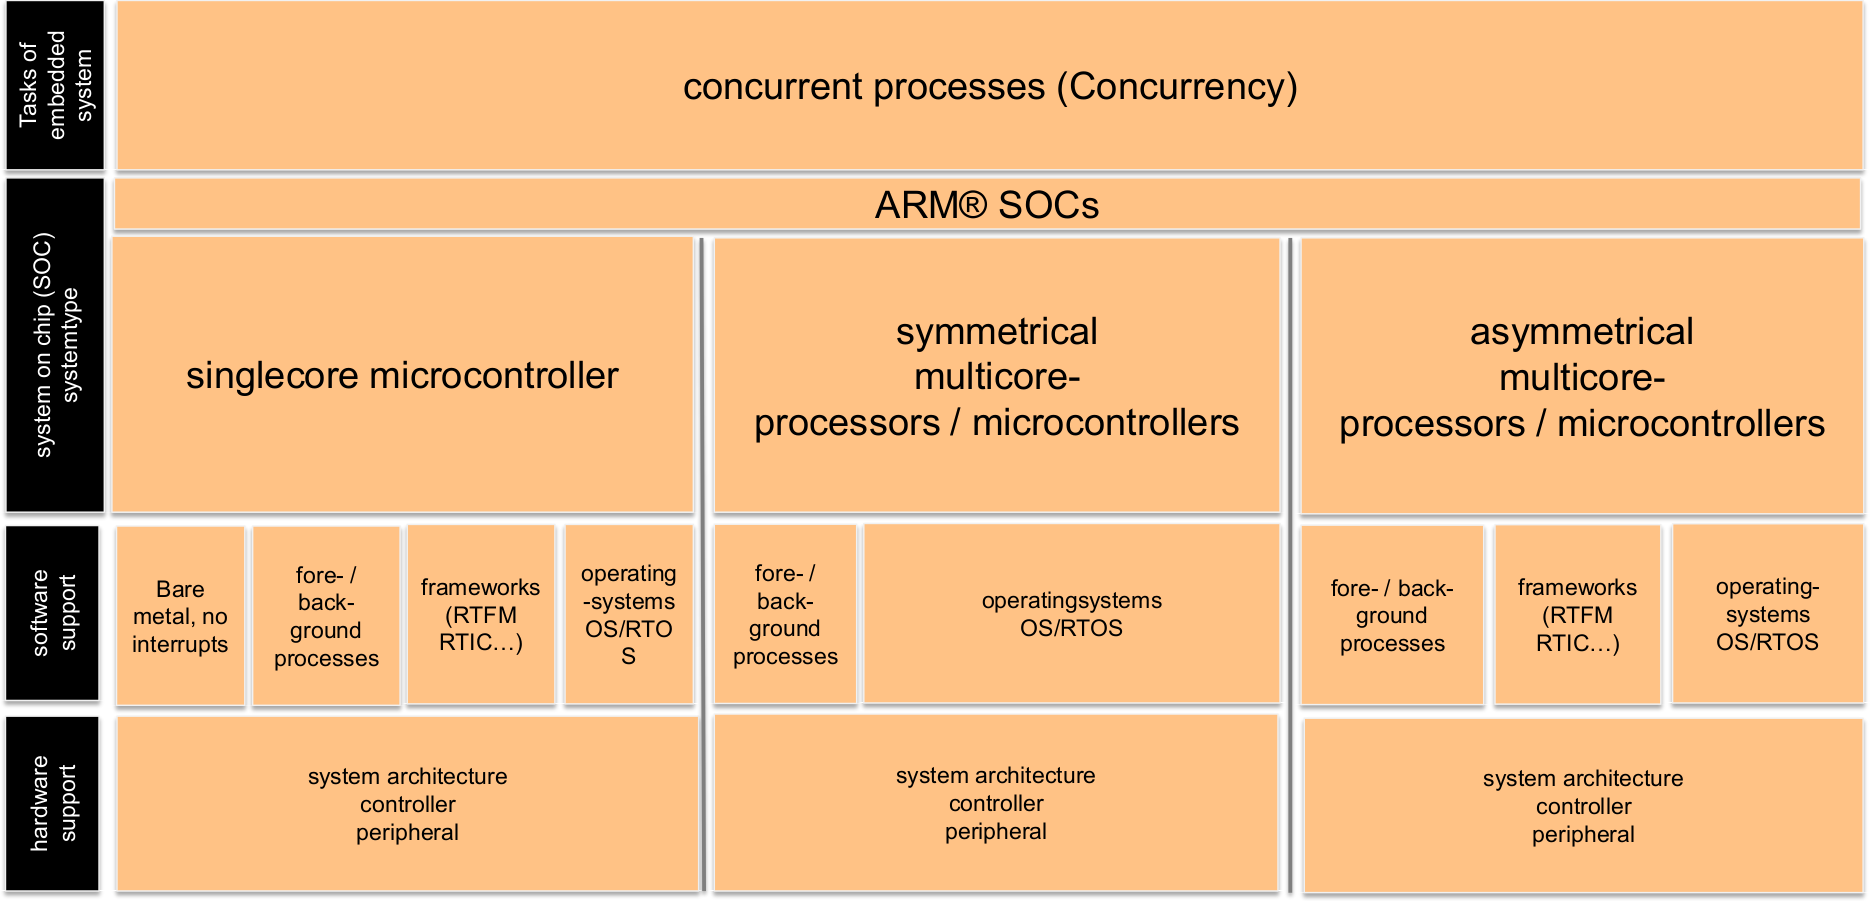
\includegraphics[width=\textwidth]{images/RTSystems/emb_landscape.png}

\subsection{Architectures}
\begin{tabularx}{\textwidth}{lXX}\hline
  Architecture & Von-Neumann                                                             & Harvard                                                             \\\hline
  Bus          & One bus for instructions and data                                       & Two seperate busses for instructions and data                       \\
  Pros         & + Cost effective design                                                 & + Better conditions for concurrency                                 \\
  Cons         & - Slower                                                                & - Costly                                                            \\
               & 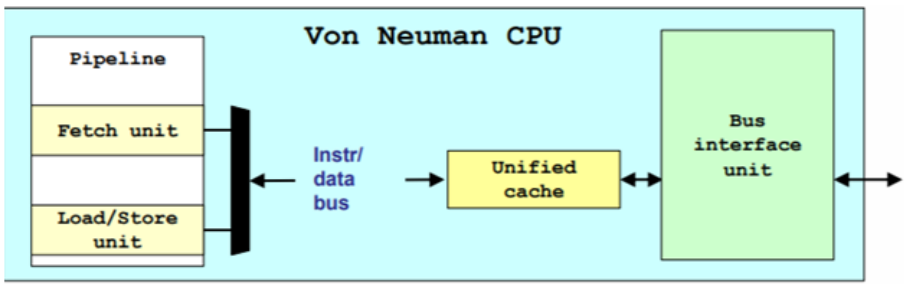
\includegraphics[width=0.4\textwidth]{images/RTSystems/von_neumann.png} & 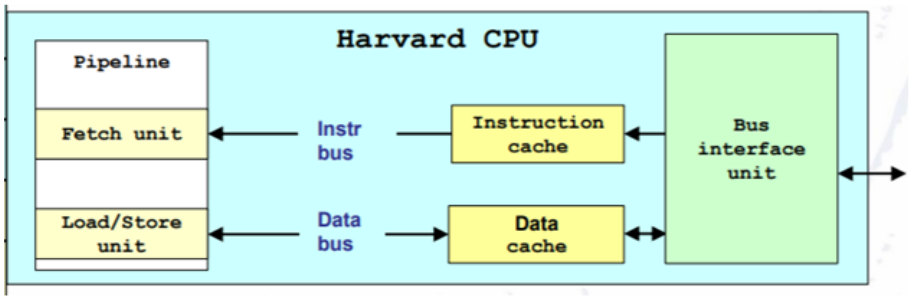
\includegraphics[width=0.4\textwidth]{images/RTSystems/harvard.png} \\\hline
\end{tabularx}

Real time support of hardware depends on:
\begin{itemize}
  \item Bus architecture
  \item CPU commands
  \item Interrput controller
\end{itemize}
%!TEX root = ../EmbSW1.tex
\section{Concurrency}
\subsection{Introduction}
\subsubsection{Motivation}
Practical programs usually perform several jobs \glqq simultaneously\grqq.

\subsubsection{Definitions}
\begin{description}
  \item[Definition:] Concurrency refers to the ability of a system to process or execute processes independently of each other.
        (Concurrency $\rightarrow$ Tasks/Processes $\rightarrow$ Threads)
  \item [Interrupt latency:] Refers to the interval of time from an external interrupt request signal being raised to the first ISR instruction being fetched and executed.
  \item [Interrupt response time:] Refers to the interval of time from an external IRQ signal being raised to the completion of the IRQ.
\end{description}
A key feature of embedded systems is the ubiquity of concurrency in applications.

\subsubsection{Parallel vs. Concurrent Computing}
\begin{itemize}
  \item Parallel Computing
        \begin{itemize}
          \item execution of different tasks is really at the same time
          \item is not possible on a single-core machine
        \end{itemize}
  \item Concurrent Computing
        \begin{itemize}
          \item execution of different tasks only seems to be at the same time
          \item different tasks get consecutive time slices
          \item there's only one task really running at a particular time slice
          \item can be done on a single- or multicore machine
        \end{itemize}
\end{itemize}

\subsubsection{Reasons to not use Concurrency}
\begin{itemize}
  \item \textbf{Concurrency (with Processes, Tasks, Threads) always cost}:
        \begin{itemize}
          \item Stack
          \item Context switch
                \begin{itemize}
                  \item takes time
                  \item Old context needs to be stored, new context needs to be loaded
                \end{itemize}
          \item Access to shared resources needs to be synchronized
                \begin{itemize}
                  \item costs
                  \item prone to errors (is forgotten or done wrong)
                \end{itemize}
        \end{itemize}
  \item \textbf{Complexity increases}
        \begin{itemize}
          \item Sequential progams are easier to understand than parallel ones.
          \item The goal should always be to keep a system as simple as possible.
        \end{itemize}
\end{itemize}

\subsection{Causes of Interrupt Latency}
For most processor architectures, the processor usually completes the current instruction, which may be a multi-cycle instruction.
\begin{itemize}
  \item To save the current scene to restore the states when returning from the ISR, the processor pushes various necessary core registers (usually the program counter, flag registers, linker register, and so on) to the stack.
  \item Some processor architectures need additional software statements to select the right ISR.
  \item Time to fetch and decode the ISR instructions to fill the pipeline.
  \item Most memory systems that store the code (such as flash) usually have wait states because the memory system clock frequency is usually much slower than the CPU clock.
  \item The interrupt may be preempted by other higher-priority interrupts anytime, including before the first ISR instruction is executed.
\end{itemize}


\subsection{Interprocess Communication (IPC)}
In a multitasking system there may exist tasks that need to cooperate with each other by exchanging messages.
This is called intertask communication, which can be classified into two types:
\begin{description}
  \item[Synchronous:] The sender and receiver need to wait for each other until the message transmission is complete.
  \item[Asynchronous:] The sender may continue to execute its next instruction while the message is being delivered to the receiver.
\end{description}
Example of asynchronous intertask communication: message queues, pipes, sockets, and signaling.

\subsubsection{Pipes}
Pipes are simple message transfer mechanism.
Mostly used for communication between two objects.
\begin{itemize}
  \item A pipe is a container of unstructured bytes.
  \item A Pipe is a strictly FIFO buffer.
  \item A pipe is a kernel object that can be a named pipe or an unnamed pipe
\end{itemize}
\glqq{}Pipes\grqq provide a task-to-task, task-to-interrupt, and interrupt-to-task communication mechanism.
However, the features of Pipes depend on the technology used.

\paragraph{Usage Patterns}
\columnratio{0.6}
\begin{paracol}{2}
  \textbf{Unidirectional Communication:} Task A writes and task B reads from pipe.
  The pipe delivers everything to manage the data flow (full, empty, data available).
  \switchcolumn
  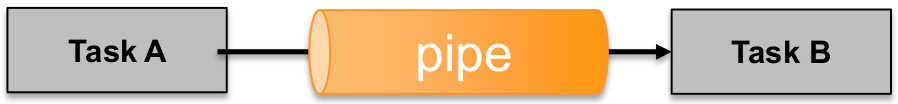
\includegraphics[width=0.39\textwidth]{images/Concurrency/uni_pipe.png}
  \switchcolumn
  \textbf{Bidrectional Communication:} Two pipes are needed to realize this pattern.
  \switchcolumn
  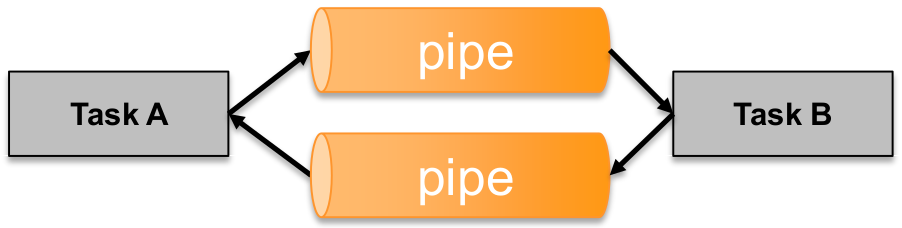
\includegraphics[width=0.39\textwidth]{images/Concurrency/bi_pipe.png}
\end{paracol}

\subsubsection{Queues}
Queues are an underlying mechanism beyond all tasks communication or synchronization in an operating system.
They are an important subject to understand as it is unavoidable to be able to build a complex application with tasks cooperating with each other.
They are a mean to store a and finite number (named \glqq{}length\grqq) of fixed size data.
They are able to be read and written by several different tasks, and don't belong to any task in particular.
A queue is normally a FIFO which means elements are read in the order they have been written.
This behavior depends on the writing method: two writing functions can be used to write either at the beginning or at the end of this queue.
\begin{itemize}
  \item A message queue is a container of multiple messages, each of which can be manipulated by a task separately.
  \item Each message in a message queue is associated with a priority; consequently, messages can be processed by tasks in priority order.
  \item A message queue is a named kernel object, with a name uniquely defined in the kernel’s namespace.
\end{itemize}
\glqq{}Queues\grqq provide a task-to-task, task-to-interrupt, and interrupt-to-task communication mechanism.
However, the features of Queues depend on the technology used (FreeRTOS supports less features).

\paragraph{Usage Patterns}
\columnratio{0.6}
\begin{paracol}{2}
  \textbf{Unidirectional Communication:} Task A writes and task B reads from queue.
  The queue delivers everything to manage the data flow (full, empty, data available).
  \switchcolumn
  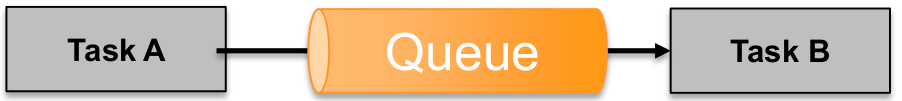
\includegraphics[width=0.39\textwidth]{images/Concurrency/uni_queue.png}
  \switchcolumn
  \textbf{Acknowledged Unidirectional Communication:}
  Similar approach as unidirectional communication, except that there is a semaphore used to signal that data was successfully received.
  Otherwise, a repetition can be triggered by task A.
  \switchcolumn
  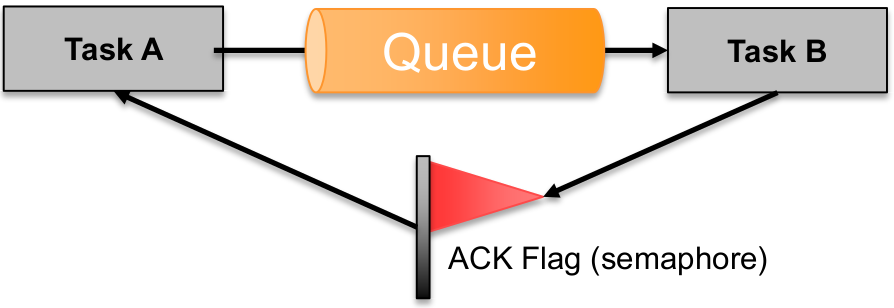
\includegraphics[width=0.39\textwidth]{images/Concurrency/ack_queue.png}
  \switchcolumn
  \textbf{Bidrectional Communication:} Two queues are needed to realize this pattern.
  \switchcolumn
  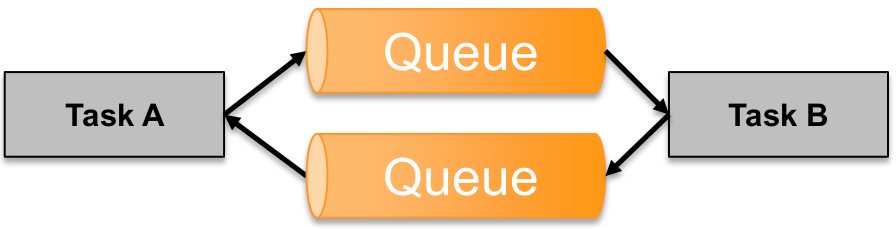
\includegraphics[width=0.39\textwidth]{images/Concurrency/bi_queue.png}
\end{paracol}


\subsection{Resource Sharing}
\subsubsection{Definitions}
\begin{description}
  \item[Race Condition]  The result of an operation depends on the timing behaviour of a specific operation.
  \item[Starvation]      Is a condition where a process never gets to it (it starves).
        The fairness condition states that starvation must be prevented.
  \item[Deadlock]        Is a situation where two processes block each other.
        A deadlock can be avoided by having all processes request the shared resources always in the same order.
  \item[Shared Variable] If the variable is accessible by all process, then the access is easy to establish.
        However race conditions can occur and data integrity is an issue.
  \item[Shared Memory] An object (a regular file or memory object) can be directly mapped into the address space of one or more processes.
        Memory mapping makes the mapped region of the object directly addressable by a process.
        This eliminates unnecessary data read, write, or copy operations, and thus offers an efficient means of passing data between processes running on the same machine.
        However shared memory is also a shared resource.
        Therefore, Resource management mechanism must be used for usage of the shared memory.
        Depending on the used technology (OS, language architecture) these mechanism are included in the shared memory object.
  \item[Priority Inversion] POSIX-compliant RTOSs implement a priority-based preemptive scheduler, which ensures that among all the threads that are ready to run, the one with the highest priority is always the task that is actually running.
        When a higher-priority thread is released, the scheduler will preempt the currently running thread in the middle of its execution.
        However, priority-based preemptive scheduling could be compromised when tasks share exclusive resources that are protected by locks:
        Requesting a resource locked by a lower-priority task would prevent a higher-priority ready task from running when it should.
        This issue is called priority inversion, referring to the phenomenon where a higher-priority task must wait for the lower-priority task.
        Priority inversion is a critical issue because it may lead to the missing of task deadlines.
\end{description}
Shared memory support:
\begin{description}
  \item[Linux, Mac, Windows:] Support shared memory in the IDEs
  \item[OpenMP:] Software library for C and C++ delivers also support for shared memory
  \item[FreeRTOS:] No explicit support of shared memory
  \item[CMSIS RTOS2:] Example to implement a shared memory: \href{https://arm-software.github.io/CMSIS_5/RTOS2/html/rtos_api2.html}{MemoryPool}
\end{description}

\subsubsection{Prevention}
\paragraph{Race Conditions}
\begin{description}
  \item[Critical Sections] Define sections in which ISR(s) are blocked.
        Pro: Simple, possible on any MCU.
        Cons: Acts blocking.
  \item[Atomic Operations] Command disables ISR for one instruction cycle.
        Atomic commands can not be split in instruction cycles that can be interrupted.
        Atomic by CPU architecture see RISC-V RV32A Atomic Extension.
        Atomic by programming language.
        \textbf{Atomic operation} is a \textbf{foundation} for all other solutions of OS and RTOS.
\end{description}

\paragraph{Deadlock}
\begin{enumerate}
  \item fixed sequence for all task on locking and unlocking the same resources.
        Example: task A and B both first lock resource 1 and then resource 2
  \item Try with return.
        Example tas A and B try to lock resource 2.
        If resource 2 is already locked, then the tasks release resource 1
  \item Timed release.
        Example: task A and B try to lock resource 2.
        If resource 2 is not available after a defined time, then the task releases resource 1 again.
  \item Atomic or Critical Section
        Example: taskk A and B lock resource 1 and resource 2 in an atomic manner or a critical section defined sequence.
\end{enumerate}

\paragraph{Priority Inversion}
\begin{description}
  \item[Priority inheritance Protocol (PIP):] When a low priority task is holding a resource and a higher priority task wants it.
        Then the priority is inherited from the higher priority tas to the lower one.
        Inheritance is also possible over several tasks, where the highest priority is inherited.
  \item[Highest Locker Protocol (HLP):] When a task takes a resource then its priority is dynamically set to the highest priority of the task pool which can take the resource.
        (also kwnown as immediate priority inheritance, immediate ceiling priority or priority protect protocol)
  \item[Priority Ceiling Protocol (PCP):] Combines PIP and HLP.
        When a low priority task is holding a resource and a higher priority task wants it then the priority is inherited from the highest priority of the task pool which can take the resource.
\end{description}

\subsubsection{Semaphores}
A semaphore an be used in various ways
\begin{itemize}
  \item Task synchronization (binary)
  \item Task ISR synchronization (binary)
  \item Counting events (counting)
  \item Flow control (share memory \& binary/counting)
  \item Resource management (binary/counting)
\end{itemize}

\paragraph{Binary Semaphore}
Binary semaphores are the simplest effective way to synchronize tasks, an other even more simple, but not as effective, consists in polling an input or a resource.
A binary semaphore can be seen as a queue which contains only one element.

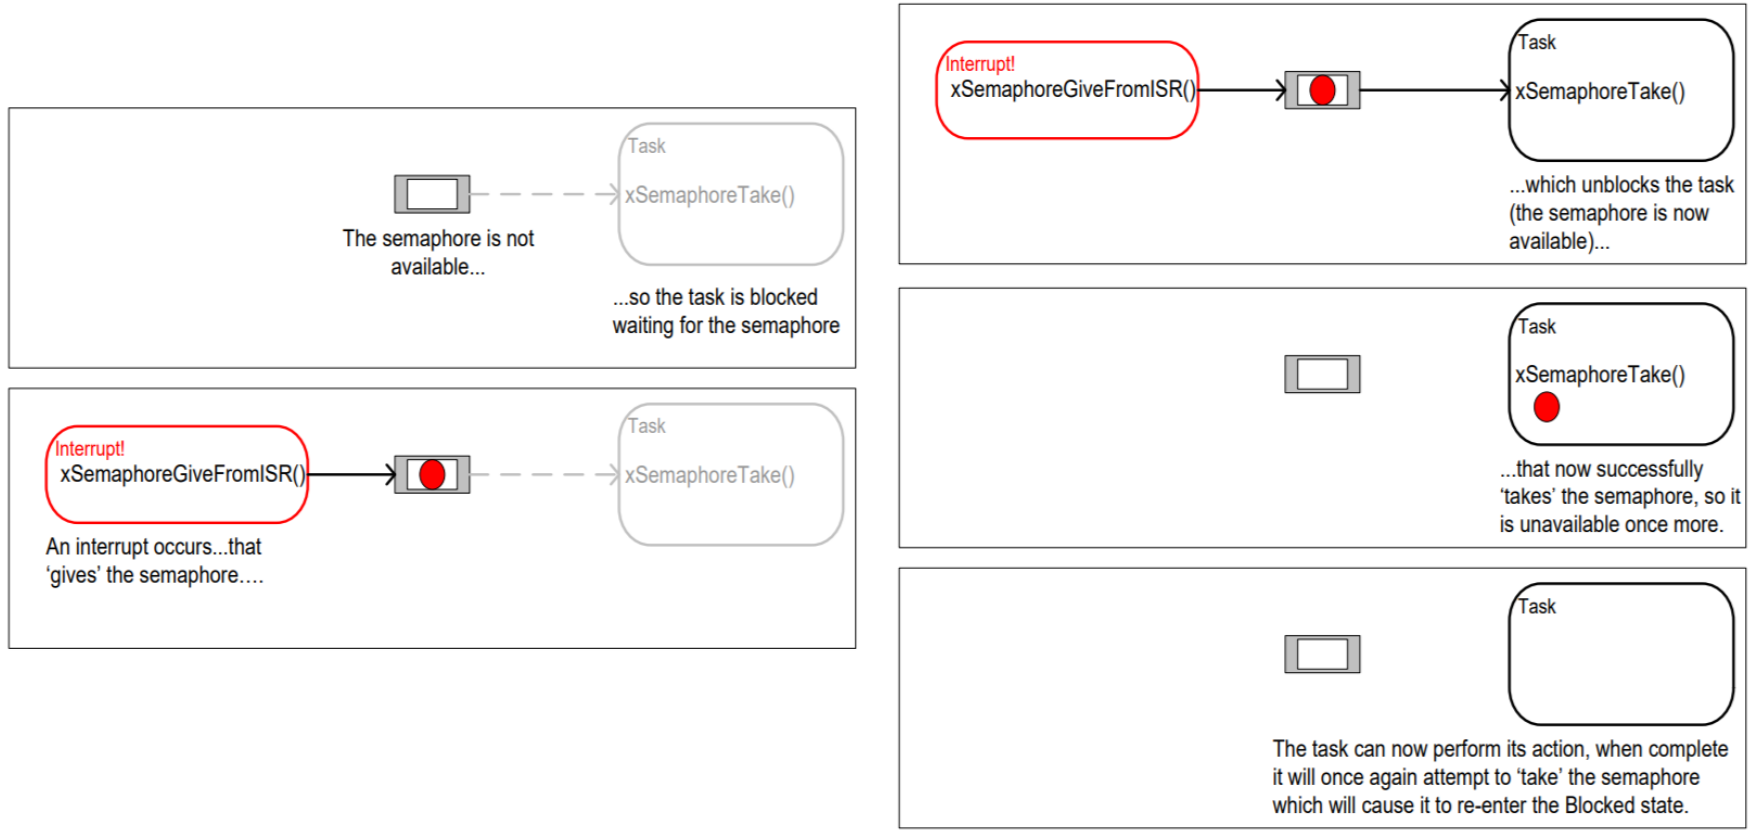
\includegraphics[width=\textwidth]{images/Concurrency/binary_semaphore.png}

\paragraph{Counting Semaphore}
A counting semaphore is a semaphore that can be taken several (but limited) times before it becomes unavailable.
It maintains a value which is increased as the semaphore is given, and decreased when it is taken.
Is is comparable to a queue with a certain amount of elements.
When created, a counting semaphore can be initialized to be available an arbitrary number of times.
The initial value and the maximum are defined on semaphore creation!

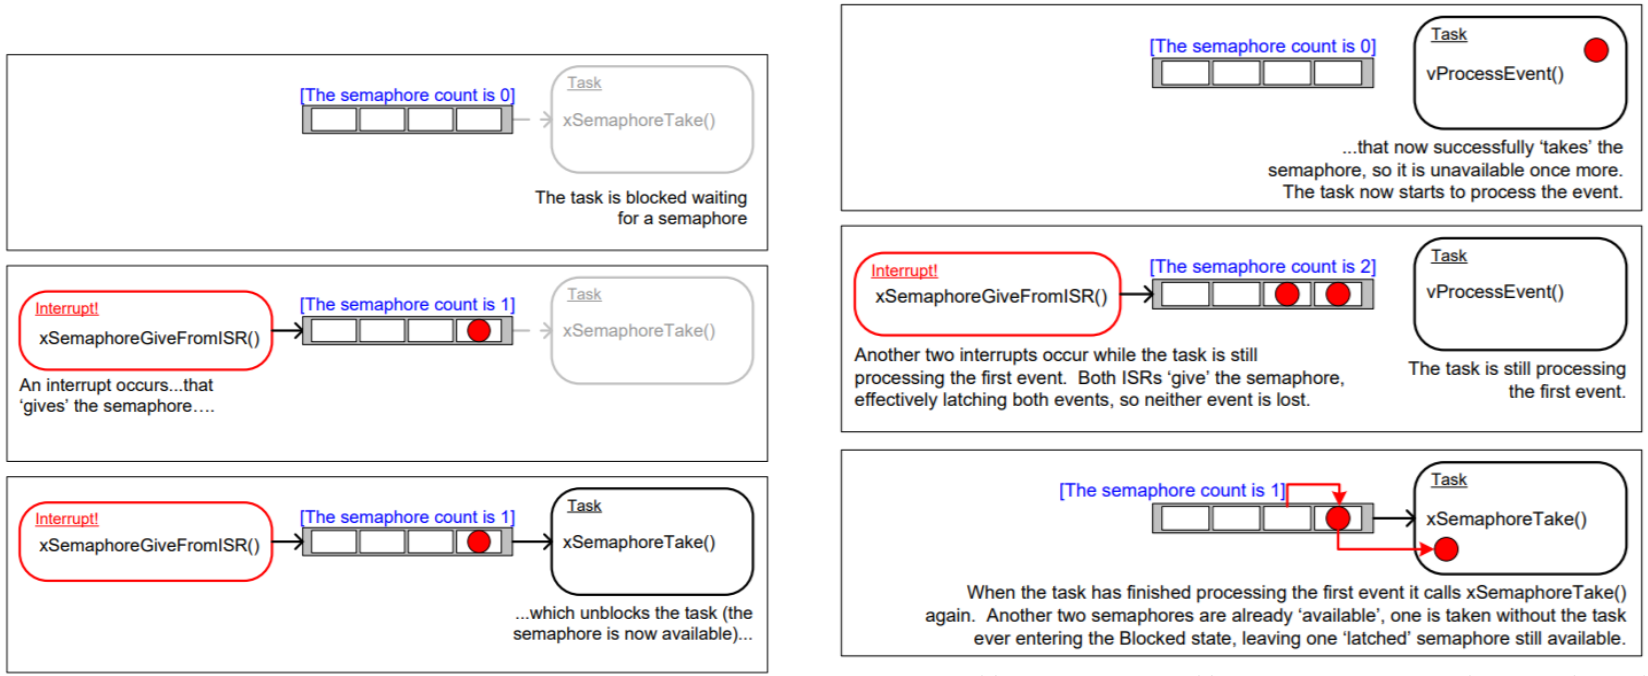
\includegraphics[width=\textwidth]{images/Concurrency/counting_semaphore.png}

\paragraph{Recommandations}
\begin{enumerate}
  \item Lock and release of Resources with semaphores costs time $\leftarrow$ less semaphores but bigger blocking regions
  \item If more tasks access semaphores, then blocking time gets longer.
        More semaphores smaller blocking regions
  \item Approach 1 and 2 are counter rotating.
        Case-specific decision, partly experimental
\end{enumerate}
In principle, it is important to create minimum locking times in order to avoid unnecessary blocking time.

\subsubsection{Mutexes}
A mutex (= mutual exclusion) is used similarly to a binary semaphore, except the task which take the semaphore must give it back.
This can be though with a token associated with the resource to access to.
A task holds the token, works with the resource then gives back the token; in the meanwhile, no other token can be given to the mutex.
Mutexes are mostly implemented blocking.

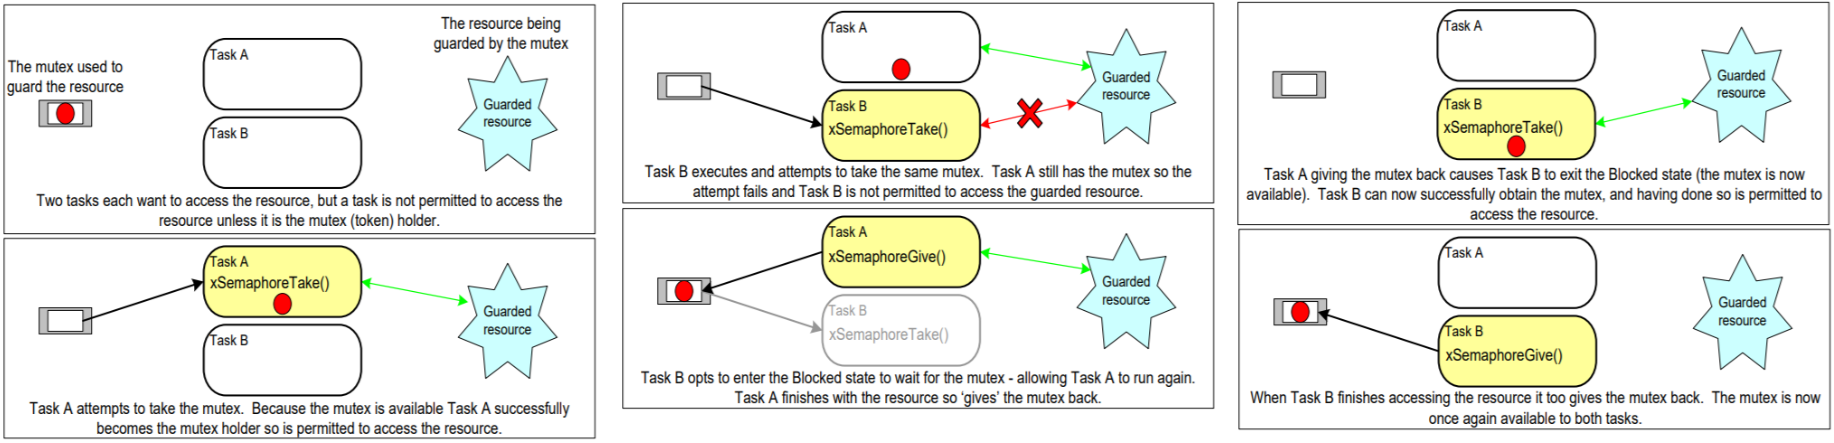
\includegraphics[width=\textwidth]{images/Concurrency/mutex.png}

\subsubsection{Recursive Mutex}
The issue arises when a task several times locks the mutex.
Consequently, it will also several time unlock the mutex.
If locking can only be done once all following locks are not counted.
If a unlock command arises the the mutex is released even if a task logic has locked it for it.

Solution:
Every lock of the mutex is counted and must be unlocked to release the mutex.
A recursive Mutex is a counting Mutex!


\subsection{Function Reentrancy}
In an RTOS the function should be thread safe:
A function is \glqq{}reentrant\grqq{} or thread safe if it is safe to call the function from more than one task, or from both tasks and interrupts.
Reentrant functions are said to be \glqq{}thread safe\grqq{} because they can be accessed from more than one thread of execution without the risk of data or logical operations becoming corrupted.
Each task maintains its own stack and its own set of processor (hardware) register values.
If a function does not access any data other than data stored on the stack or held in a register, then the function is reentrant, and thread safe.

That's also a reason why there are different implementations of functions for ISR and tasks.
% \textbf{Folgerung:} Concurrency nur dann einsetzen, wenn wirklich ein Nutzen vorhanden ist!\\
% Tendenziell werden speziell bei Verwendung eines RTOS zu viele Threads definiert, welche das System nur komplexer und komplizierter machen $\rightarrow$ \textbf{Sequential} is simple, \textbf{concurrent} is error-prone

% \subsection{POSIX Threads Programming}
% \subsubsection{UNIX Process}
% \begin{itemize}
%   \item Heavyweight process (created by the operating system)
%   \item Processes require a fair amount of overhead; they contain information about program resources and program execution state, including: Process ID, process group ID, user ID, and group ID; Environment; Program instructions; Registers; Stack; Heap; File descriptors; Signal actions; Shared libraries; Inter-process communication tools
% \end{itemize}

% \subsubsection{UNIX Thread}
% \begin{itemize}
%   \item Lightweight "'process"'
%   \item \textbf{Threads use and exist within the process resources}
%   \item \textbf{A thread uses the same address space as other threads of the same process}
%   \item Threads are able to be scheduled by the operating system
%   \item Independent stream of instructions that may run simultaneously to other streams of instructions
%   \item Procedure that runs independently from its main program
%   \item A thread maintains its own: Stack pointer; Registers; Scheduling properties; Set of pending and blocked signals; Thread specific data
%   \item Concurrent programs are usually achieved with threads
% \end{itemize}

% \subsubsection{Process vs. Thread in UNIX}
% 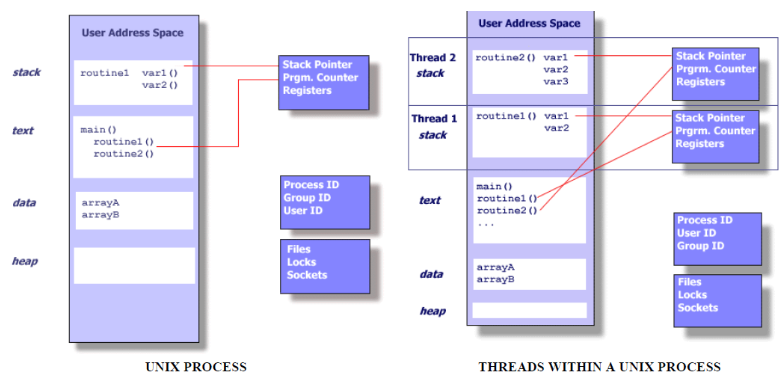
\includegraphics[width=12cm]{images/Concurrency/ProcessVsThread.png}\\\\
% Man beachte: Alles was ein Thread inne hat, hat ein Prozess auch inne (aber NICHT umgekehrt)!

% \subsection{What are POSIX Threads?}
% \begin{itemize}
%   \item For UNIX systems, a standardized C language threads programming interface has been specified by the \textbf{IEEE POSIX 1003.1c standard}.
%   \item The short form of \textbf{POSIX threads} is \textbf{Pthreads} or \textbf{pthreads}.
%   \item When compared to the cost of creating and managing a process, a thread can be created with much less operating system overhead
%   \item Managing threads requires fewer system resources than managing processes
% \end{itemize}

% \subsubsection{The pthreads API}
% \begin{itemize}
%   \item Routines of the pthreads API start with \textbf{pthread\_}
%   \item The header file \textbf{pthread.h} must be included
%   \item Source files that use pthreads shall be compiled and linked with \textbf{-pthread}
%   \item The link command must include \textbf{–lpthread}
% \end{itemize}

% \subsubsection{Starting and Terminating a Thread}
% \begin{itemize}[noitemsep,topsep=0pt]
%   \item Any routine with the following interface may become a thread routine: \lstinline{void* threadRoutine(void* arg);}
%   \item A thread is started with:\newline
%         \lstinline{int pthread_create(pthread_t* thread, const pthread_attr_t* attr, void* (*startRoutine) (void*), void* arg);}
%         \begin{itemize}[noitemsep,topsep=0pt]
%           \item thread: pointer to a pthread\_t instance
%           \item attr: pointer to a pthread\_attr\_t structure, often 0 (default attributes)
%           \item arg: a single argument that may be passed to startRoutine
%           \item returns 0 on success
%         \end{itemize}
%   \item A thread terminates in one of the following ways:
%         \begin{itemize}[noitemsep,topsep=0pt]
%           \item it calls pthread\_exit()
%           \item it returns from startRoutine
%           \item it is canceled with pthread\_cancel()
%         \end{itemize}
% \end{itemize}

% \textbf{Example - Starting a Thread}
% \begin{lstlisting}[style=C, escapechar=!]
% #include <pthread.h>
% void* threadFunction(void* arg);
% int main(void)
% {
%   pthread_t myT; !\tikz[remember picture] \node [] (a) {};!
%   int ret = pthread_create!\tikz[remember picture] \node [] (b) {};!(&myT, 0, threadFunction, 0);
%   if (ret)
%   {  // handle error
%     return -1;
%   }
%   while (1) {} // endless loop
%   pthread_exit(0);
% }
% void* threadFunction(void* arg)
% {  // implement this
%   pthread_exit(0);
% }
% \end{lstlisting}
% \begin{tikzpicture}[remember picture, overlay,
%     every edge/.append style = { ->, thick, >=stealth, dashed, line width = 1pt},
%     every node/.append style = { align = left, minimum height = 10pt, font = \bfseries, fill= green!20},
%     text width = 5.5cm]
%   \node [right=8cm of a] (A) {myT becomes the reference to the thread};
%   \node [below right=.5cm and 3cm of b, text width=8.5cm] (B) {starts thread and immediately returns (thread may not yet be fully started)};
%   \draw (A.west) edge (a.east);
%   \draw[->, to path={-| (\tikztotarget)}] (B.west) edge (b.south);
% \end{tikzpicture}

% \textbf{Example - Waiting on a Thread to Finish}
% \begin{lstlisting}[style=C, escapechar=!]
% #include <pthread.h>
% void* threadFunction(void* arg);
% int main(void)
% {
%   pthread_t myT;
%   pthread_attr_t attr;
%   pthread_attr_init(&attr); // initialize and set thread detached attribute
%   pthread_attr_setdetachstate(&attr, PTHREAD_CREATE_JOINABLE);
%   int ret = pthread_create(&myT, &attr, threadFunction, 0); // only starts and returns
%   if (ret)
%   {  // handle error
%     return -1;
%   }
%   pthread_attr_destroy(&attr); // free attribute
%   ret = pthread_join(myT, 0);!\tikz[remember picture] \node [] (a) {};!
%   if (ret)
%   {  // handle error
%     return -1;
%   }
%   pthread_exit(0);
% }
% void* threadFunction(void* arg)
% {  // implement this
%   pthread_exit(0);
% }
% \end{lstlisting}
% \begin{tikzpicture}[remember picture, overlay,
%     every edge/.append style = { ->, thick, >=stealth, dashed, line width = 1pt},
%     every node/.append style = { align = left, minimum height = 10pt, font = \bfseries, fill= green!20},
%     text width = 7.5cm]
%   \node [right=5cm of a] (A) {main thread waits on myT to finish};
%   \draw (A.west) edge (a.east);
% \end{tikzpicture}
% %\lstinputlisting[style=C]{snippets/Threads/thread_waiting.c}

% \subsubsection{Thread-safeness}
% \begin{itemize}
%   \item Thread-Sicherheit besagt, dass eine Komponente gleichzeitig von verschiedenen Programmbereichen mehrfach ausgeführt werden kann, ohne dass diese sich gegenseitig behindern.
%   \item Änderungen der einzelnen Threads müssen koordiniert werden, um einen chaotischen Zustand des Speichers zu verhindern, da das Programm dabei häufig gleichzeitig auf einen gemeinsamen Speicherbereich (Shared Memory) des Computers zugreifen will.
%   \item Vorsicht: rand() ist nicht thread-safe (weil bei dieser Fkt. eine interne Variable verwendet wird, welche schon zum Voraus berechnet wurde); rand\_r() hingegen schon.
% \end{itemize}

% \subsubsection{Quasiparallelität und "'Prozess"'-Zustände}
% \begin{minipage}[c]{8cm}
%   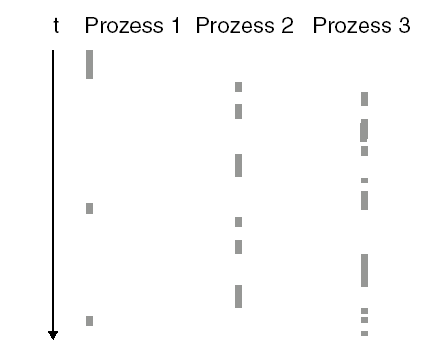
\includegraphics[width=5cm]{images/Concurrency/Quasiparallelitaet.png}
% \end{minipage}
% \begin{minipage}[c]{10cm}
%   \begin{itemize}
%     \item Prozesse/Threads warten die meiste Zeit (blocked).
%     \item Scheduler ordnet CPU denjenigen Prozessen/Threads zu, die im Zustand ready sind und "'etwas zu tun haben"'
%   \end{itemize}
% \end{minipage}\\\\
% Prozesse/Threads können folgende Zustände und Übergänge erfahren:\\
% \begin{minipage}[c]{8cm}
%   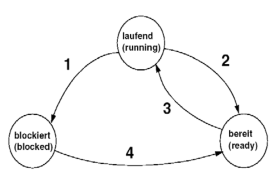
\includegraphics[width=6cm]{images/Concurrency/Prozesszustaende.png}
% \end{minipage}
% \begin{minipage}[c]{10cm}
%   \begin{enumerate}
%     \item I/O Operation, Warten auf Bedingung
%     \item Scheduler entzieht CPU
%     \item Scheduler weist CPU zu
%     \item I/O beendet, Bedingung erfüllt
%   \end{enumerate}
% \end{minipage}

% \subsection{Synchronisation: Zugriff auf gemeinsame Ressourcen}
% \subsubsection{Kritischer Abschnitt (Critical Section, CS)}
% \begin{itemize}
%   \item Codebereich, in dem nebenläufige oder parallele Prozesse auf gemeinsame Ressourcen zugreifen. Zu jeder Zeit darf sich höchstens ein Prozess im kritischen Bereich
%         befinden.
%   \item Der exklusive Zugriff durch höchstens einen Prozess wird mittels gegenseitigem Ausschluss (mutual exclusion, Mutex) sichergestellt.
% \end{itemize}

% \subsubsection{Lösungsstruktur für gegenseitigen Ausschluss}
% \begin{minipage}[c]{2cm}
%   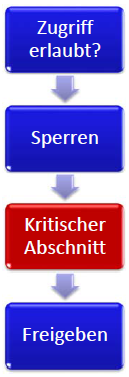
\includegraphics[width=1.5cm]{images/Concurrency/Loesungsstruktur.png}
% \end{minipage}
% \begin{minipage}[c]{14cm}
%   \begin{itemize}
%     \item Bei der Zugriffsprüfung wird gewartet, bis der Zugang frei wird \\ \ \\
%     \item Beim Sperren wird das Signal auf Rot gesetzt (lock a mutex) \\ \ \\
%     \item Beim Freigeben wird das rote Signal wieder gelöscht (unlock a mutex)
%   \end{itemize}
% \end{minipage}

% \subsubsection{Forderungen an die Synchronisation (Dijkstra, 1965)}
% \begin{enumerate}
%   \item Es dürfen sich nicht zwei Prozesse gleichzeitig in ihrem kritischen Abschnitt befinden (mutual exclusion).
%   \item Über die Abarbeitungsgeschwindigkeit, bzw. die Anzahl Prozesse dürfen keine Annahmen getroffen werden.
%   \item Kein Prozess darf ausserhalb eines kritischen Abschnitts einen anderen Prozess blockieren.
%   \item Jeder Prozess, der am Eingang eines kritischen Abschnitts wartet, muss irgendwann den Abschnitt betreten dürfen (fairness condition).
% \end{enumerate}

% % \begin{tabbing}
% %   \hspace*{1cm}\=\hspace*{4.2cm}\=\hspace*{3cm}\=\hspace*{2.7cm}\= \kill
% % \textbf{Synchro-Versuch 1}\\\\
% %   \>{\textbf Prozess 1} \> \> \>{\textbf Prozess 2}\\
% %   \>\begin{lstlisting}[style=C]
% % while(grant != 1)
% %     wait();
% % CS; //Eintritt in Critical Section
% % grant = 2;
% %     \end{lstlisting} \> \> \>
% %     \begin{lstlisting}[style=C]
% % while(grant != 2)
% %     wait();
% % CS; //Eintritt in Critical Section
% % grant = 1;
% %     \end{lstlisting} \\\\
% %     Forderung 2 nicht erfüllt, da sich alle Prozesse selbst daran hindern 2mal nacheinander daran zu kommen.\\\\
% %
% % \textbf{Synchro-Versuch 2}\\\\
% %    \>{\textbf Prozess 1} \> \> \>{\textbf Prozess 2}\\
% %    \>\begin{lstlisting}[style=C]
% % while(in2)
% %     wait();
% % in1 = true;
% % CS; //Eintritt in Critical Section
% % in1 = false;
% %     \end{lstlisting} \> \> \>
% %     \begin{lstlisting}[style=C]
% % while(in1)
% %     wait();
% % in2 = true;
% % CS; //Eintritt in Critical Section
% % in2 = false;
% %     \end{lstlisting} \\\\
% %     Initialisierung ist nicht gelöst.\\\\
% %
% % \textbf{Synchro-Versuch 3 (Algorithmus von Peterson)}\\\\
% %    \>{\textbf Prozess 1} \> \> \>{\textbf Prozess 2}\\
% %    \>\begin{lstlisting}[style=C]
% %         request1 = true;
% %         grant = 1;
% %         while(grant==1 && request2)
% %           wait();
% %         CS; //Eintritt in Critical Section
% %         request1 = false;
% %     \end{lstlisting} \> \> \>
% %     \begin{lstlisting}[style=C]
% %         request2 = true;
% %         grant = 2;
% %         while(grant==2 && request1)
% %           wait();
% %         CS;  //Eintritt in Critical Section
% %         request2 = false;
% %     \end{lstlisting} \\
% % \end{tabbing}
% % \vspace*{-1cm}

% \subsubsection{Synchronisation mit Signalen}
% \begin{itemize}
%   \item Jeder Prozess wartet vor Betreten des kritischen Bereichs auf ein
%         gemeinsames Signal.
%   \item Wenn Signal gesetzt $\rightarrow$ kritischer Bereich frei
%   \item waitfor(signal) blockiert aufrufenden Prozess, falls signal nicht
%         gesetzt
%   \item Jeder Prozess, der fertig ist, setzt Signal mit send(signal)
%   \item Mehrere Prozesse können gleichzeitig warten
%   \item Es ist Aufgabe des Schedulingalgorithmus' bei gesetztem Signal einem der wartenden Prozesse das Betreten des kritischen Abschnitts zu gewähren
% \end{itemize}

% \begin{tabbing}
%   \hspace*{1cm}\=\hspace*{4.2cm}\=\hspace*{3cm}\=\hspace*{2.7cm}\= \kill
%   \>{\textbf Prozess 1} \> \> \>{\textbf Prozess 2}\\
%   \>\begin{lstlisting}[style=C]
% waitFor(signal);
% CS;  //Eintritt in Critical Section
% send(signal);
%     \end{lstlisting} \> \> \>
%   \begin{lstlisting}[style=C]
% waitFor(signal);
% CS;  //Eintritt in Critical Section
% send(signal);
%     \end{lstlisting} \\\\
% \end{tabbing}
% \vspace*{-1.5cm}

% \subsection{Semaphoren}
% \begin{itemize}
%   \item Das Signal für den Zutritt in den kritischen Bereich = Semaphor
%   \item Ein Semaphor s hat zwei atomare (= nicht unterbrechbare)
%         Operationen
%         \begin{itemize}
%           \item P(s) : Passieren $\rightarrow$ Beim Eintritt in CS (waitFor)
%           \item V(s) : Verlassen $\rightarrow$ Beim Austritt aus CS (send)
%         \end{itemize}
%   \item Busy waiting
%         \begin{itemize}
%           \item Beim Busy Waiting warten die Prozesse aktiv in einer Schleife (spin lock)
%           \item Wartende Prozesse belasten so unnötigerweise den Prozessor
%           \item \textbf{Lösung:} Wartende Prozesse werden in eine Warteschlange eingetragen (sleep und
%                 wakeup)
%         \end{itemize}
%   \item Probleme der Semaphoren
%         \begin{itemize}
%           \item Anwendung erfordert viel Disziplin
%                 \begin{itemize}
%                   \item Für jedes P(s) braucht es auch ein V(s)
%                   \item Probleme treten auf, wenn V(s) vergessen geht! (Ressource bleibt besetzt)
%                 \end{itemize}
%           \item In grösseren Programmen können subtile Probleme entstehen, falls z.B. das V(s) in einer if-Bedingung gemacht wird.
%           \item Beim Auftreten einer Exception kann das Freigeben ebenfalls schwierig werden.
%         \end{itemize}
% \end{itemize}

% \subsection{Thread-Synchronisation in C mit POSIX Threads}
% \subsubsection{Mutual Exclusion (Mutex)}
% \begin{itemize}
%   \item A mutex variable acts like a "'lock"' protecting access to a shared data resource
%   \item The basic concept of a mutex as used in Pthreads is that only one thread can lock (or own) a mutex variable at any given time. Thus, even if several threads try to lock a mutex, only one thread will be successful.
%   \item No other thread can own that mutex until the owning thread unlocks that mutex
%   \item Very often the action performed by a thread owning a mutex is the updating of global (shared) variables
%   \item This is a safe way to ensure that when several threads update the same variable, the final value is the same as what it would be if only one thread performed the update
%   \item The variables being updated belong to a \textbf{critical section}
% \end{itemize}
% \textbf{A typical mutex sequence:}
% \begin{enumerate}
%   \item Create and initialize a mutex variable
%   \item Several threads attempt to lock the mutex
%   \item Only one succeeds and that thread owns the mutex
%   \item The owner thread performs some set of actions
%   \item The owner unlocks the mutex
%   \item Another thread acquires the mutex and repeats the process
%   \item Finally the mutex is destroyed
% \end{enumerate}

% \lstinputlisting[style=C]{snippets/Concurrency/Sync_POSIX.c}

% \subsubsection{Das Monitorprinzip}
% \begin{itemize}
%   \item Grundprinzip: Abstrakten Datenyp (ADT) definieren, der genau die Funktionen
%         in der Schnittstelle anbietet, die notwendig sind.
%   \item Der Aufrufer ruft diese Funktionen auf, er muss sich aber nicht um die
%         Synchronisation kümmern.
%   \item Die Synchronisation z.B. mit Semaphoren ist in der Implementation des
%         Monitors lokal gelöst.
%   \item Problem wird einmal im Monitor gelöst, die Aufrufer müssen sich nicht
%         mehr darum kümmern.
% \end{itemize}

% \subsubsection{Race condition/Starvation/Deadlock}
% \begin{description}
%   \item[Race Condition]  Das Ergebnis einer Operation hängt vom zeitlichen Verhalten bestimmter Einzeloperationen ab.
%   \item[Starvation]      Ist ein Zustand, bei dem ein Prozess nie dran kommt (er verhungert). Die Fairness condition besagt, dass Starvation verhindert werden muss.
%   \item[Deadlock]        Ist eine Situation in denen sich zwei Prozesse gegenseitig blockieren. Ein Deadlock kann vermieden werden, indem alle Prozesse die gemeinsamen Ressourcen immer in derselben Reihenfolge anfordern.
% \end{description}

% \subsection{Condition Variables}
% \begin{itemize}
%   \item Mutexes implement synchronization by controlling thread access to data
%   \item \textbf{Condition variables allow threads to synchronize based upon the actual value of data}
%   \item Without condition variables, the programmer would need to have threads continually polling (possibly in a critical section), to check if the condition is met
%   \item This can be very resource consuming since the thread would be continuously busy in this activity
%   \item \textbf{A condition variable is a way to achieve the same goal without polling}
%   \item A condition variable is always used in conjunction with a mutex lock
% \end{itemize}
% \begin{center}
%   \begin{minipage}{0.8\linewidth}
%     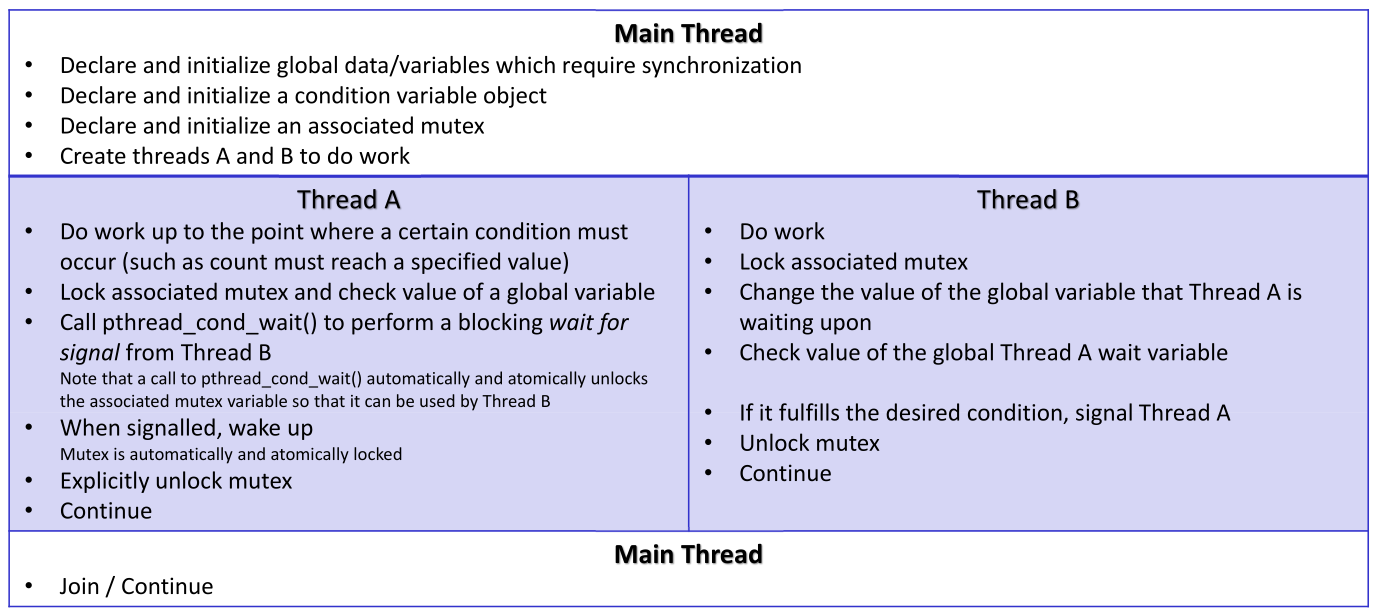
\includegraphics[width=\linewidth]{images/Concurrency/conditionVariablesAblauf}
%   \end{minipage}
% \end{center}

% \subsubsection{Creating and destroying condition variables}
% \begin{itemize}
%   \item Condition variables must be initialized before they can be used\newline
%         \lstinline{int pthread_cond_init(pthread_cond_t* condVar, const pthread_condattr_t* attr);}
%         \begin{itemize}
%           \item condVar: pointer to the condition variable
%           \item attr: pointer to a pthread\_condattr\_t structure, often 0 (default attributes)
%           \item returns 0 on success
%         \end{itemize}
%   \item The condition variables shall be destroyed when they're no longer needed\newline
%         \lstinline{int pthread_cond_destroy(pthread_cond_t* condVar);}
%         \begin{itemize}
%           \item condVar: pointer to the condition variable
%           \item returns 0 on success
%         \end{itemize}
% \end{itemize}

% \subsubsection{Waiting on condition variables}
% \begin{itemize}
%   \item waiting on condition variable: blocks calling thread until condition is signalled\newline
%         \lstinline{int pthread_cond_wait(pthread_cond_t* condVar, pthread_mutex_t* mutex);}
%         \begin{itemize}
%           \item condVar: pointer to the condition variable
%           \item mutex: pointer to the mutex
%           \item returns 0 on success
%         \end{itemize}
%   \item This routine should be called while mutex is locked
%   \item It will automatically release the mutex while it waits
%   \item After signal is received and thread is awakened, mutex will be automatically locked for use by the thread
%   \item The programmer is then responsible for unlocking mutex when the thread is finished with it
% \end{itemize}

% \subsubsection{Signaling on condition variables}
% \begin{itemize}
%   \item Signal on condition variable: unblocks thread blocked on a condition variable\newline
%         \lstinline{int pthread_cond_signal(pthread_cond_t* condVar);}
%         \begin{itemize}
%           \item condVar: pointer to the condition variable
%           \item returns 0 on success
%         \end{itemize}
%   \item This routine is used to signal (or wake up) another thread which is waiting on the condition variable
%   \item It should be called after mutex is locked, and must unlock mutex in order for pthread\_cond\_wait() routine to complete
% \end{itemize}

% \subsubsection{Using condition variables}
% \begin{itemize}
%   \item This example code demonstrates the use of several Pthread condition variable routines
%   \item The main routine creates three threads
%         \begin{itemize}
%           \item Two of the threads perform work and update a count variable
%           \item The third thread waits until the count variable reaches a specific value
%         \end{itemize}
%   \item The counting thread that reaches the specified count value signals (wakes up) the watching thread waiting on this condition
% \end{itemize}

% \lstinputlisting[style=C]{snippets/Concurrency/condVariableMain.c}
% \lstinputlisting[style=C]{snippets/Concurrency/condVariableIncCount.c}
% \lstinputlisting[style=C]{snippets/Concurrency/condVariableWatchCount.c}

% \subsubsection{Bounded Buffer Problem}
% \begin{itemize}[noitemsep,topsep=0pt]
%   \item The problem describes two processes, the producer and the consumer, who share a common, fixed-size buffer used as a queue.
%   \item The producer's job is to generate a piece of data, put it into the buffer and start again.
%   \item At the same time, the consumer is consuming the data (i.e., removing it from the buffer) one piece at a time.
%   \item The problem is to make sure that the producer won't try to add data into the buffer if it's full and that the consumer won't try to remove data from an empty buffer.
%   \item The problem can also be generalized to have multiple producers and consumers.
% \end{itemize}
% \textbf{Solution:}
% \begin{itemize}[noitemsep,topsep=0pt]
%   \item The solution for the producer is to either go to sleep or discard data if the buffer is full.
%   \item The next time the consumer removes an item from the buffer, it notifies the producer, who starts to fill the buffer again.
%   \item In the same way, the consumer can go to sleep if it finds the buffer to be empty.
%   \item The next time the producer puts data into the buffer, it wakes up the sleeping consumer.
%   \item The solution can be reached by means of inter-process/thread communication, typically using semaphores (mutexes).
%   \item An inadequate solution could result in a deadlock where both processes are waiting to be awakened.
% \end{itemize}

% \subsection{POSIX Interprocess Communication (IPC)}
% \begin{itemize}[noitemsep,topsep=0pt]
%   \item POSIX provides the following IPC mechanisms in the POSIX:XSI extension:
%         \begin{itemize}
%           \item Message queues in sys/msg.h
%           \item Semaphores in sys/sem.h
%           \item Shared Memory in sys/shm.h
%         \end{itemize}
%   \item These mechanisms allow unrelated processes to exchange information in a reasonably efficient way
% \end{itemize}

% \subsection{RAII (Resource Acquisition Is Initialisation)}
% \subsubsection{Motivation}
% \begin{itemize}[noitemsep,topsep=0pt]
%   \item Ressourcen (z.B. Datei, Speicher, etc.) müssen vor dem Gebrauch grundsätzlich angefordert werden
%   \item Nach Abschluss des Gebrauchs einer Ressource muss diese wieder freigegeben werden
%   \item Die saubere Anforderung und Freigabe ist fehlerträchtig
%   \item RAII löst diese Aufgabe elegant und zuverlässig
% \end{itemize}

% \subsubsection{Idee hinter RAII}
% \begin{itemize}[noitemsep,topsep=0pt]
%   \item Die Anforderung und Freigabe einer Ressource wird mit Hilfe einer Klasse implementiert:
%         \begin{itemize}
%           \item der Konstruktor fordert die Ressource an
%           \item der Destruktor gibt sie wieder frei
%         \end{itemize}
%   \item Die verwendete Ressource kann wie ein Objekt behandelt werden. Sobald das Objekt seine Gültigkeit verliert (z.B. out-of-scope), wird durch den Destruktor die Ressource "'automatisch"' freigegeben.
% \end{itemize}

% \subsubsection{Anwendung bei Heapobjekten}
% \begin{itemize}[noitemsep,topsep=0pt]
%   \item Wie kann man sicher gehen, dass ein Objekt, welches auf dem Heap angelegt wurde, auch wieder mittels delete sicher gelöscht wird?
%         \begin{itemize}
%           \item Exceptions können dazwischen kommen
%           \item C++03 kennt kein finally bei Exception-Handling
%         \end{itemize}
% \end{itemize}
% \begin{lstlisting}[style=C,escapechar=!]
% void f()
% {
%   Person* p = new Person("irgendwer");
%   // mach etwas mit p!\tikz[remember picture] \node [] (a) {};!
%   delete p;
% }
% \end{lstlisting}
% \begin{tikzpicture}[remember picture, overlay,
%     every edge/.append style = { ->, thick, >=stealth, dashed, line width = 1pt},
%     every node/.append style = { align = left, minimum height = 10pt, font = \bfseries, fill= green!20},
%     text width = 7.5cm]
%   \node [right=5cm of a] (A) {was ist, wenn hier eine Exception geworfen wird?};
%   \draw (A.west) edge (a.east);
% \end{tikzpicture}
% \textbf{Lösung:}
% \begin{itemize}[noitemsep,topsep=0pt]
%   \item Kapsle die dynamisch erzeugte Ressource mit einem Handle-Objekt auf dem Stack
%         \begin{itemize}[noitemsep,topsep=0pt]
%           \item Ideal std::shared\_ptr\textless T\textgreater aus Header \textless memory\textgreater
%         \end{itemize}
%   \item Der Destruktor dieses Handle-Objekts räumt beim Verlassen des Scopes automatisch auf. Das gilt auch für externe Ressourcen wie Files
% \end{itemize}
% \begin{lstlisting}[style=C,escapechar=!]
% #include <memory>
% void f()
% {
%   std::shared_ptr<Person> p(new Person("irgendwer"));
%   // mach etwas mit p
% }!\tikz[remember picture] \node [] (a) {};!
% \end{lstlisting}
% \begin{tikzpicture}[remember picture, overlay,
%     every edge/.append style = { ->, thick, >=stealth, dashed, line width = 1pt},
%     every node/.append style = { align = left, minimum height = 10pt, font = \bfseries, fill= green!20},
%     text width = 11cm]
%   \node [right=5cm of a] (A) {Beim Verlassen des Blocks räumt der Destruktor von shared\_ptr automatisch auf und löscht die Person};
%   \draw (A.west) edge (a.east);
% \end{tikzpicture}

% \subsubsection{Anwendung bei Mutex}
% \begin{itemize}[noitemsep,topsep=0pt]
%   \item Wie kann man sicher gehen, dass eine Mutex, die mit lock(m) angefordert wurde, in jedem Fall auch wieder mit unlock(m) freigegeben wurde?
%         \begin{itemize}
%           \item Exceptions können dazwischen kommen
%           \item Freigabe auch bei vorzeitigem Ausstieg mit return
%         \end{itemize}
% \end{itemize}
% \begin{lstlisting}[style=C,escapechar=!]
% static pthread_mutex_t m;
% // ...
% void f()
% {
%   pthread_mutex_lock(&m);
%   // mach etwas in kritischem Abschnitt!\tikz[remember picture] \node [] (a) {};!
%   pthread_mutex_unlock(&m);   // auf keinen Fall vergessen
% }
% \end{lstlisting}
% \begin{tikzpicture}[remember picture, overlay,
%     every edge/.append style = { ->, thick, >=stealth, dashed, line width = 1pt},
%     every node/.append style = { align = left, minimum height = 10pt, font = \bfseries, fill= green!20},
%     text width = 6.5cm]
%   \node [right=4cm of a] (A) {was ist, wenn hier eine Exception geworfen wird?};
%   \draw (A.west) edge (a.east);
% \end{tikzpicture}
% \textbf{Lösung:}\\
% Kritischer Abschnitt muss in einen Block gepackt werden.
% \begin{lstlisting}[style=C,escapechar=!]
% class ResourceLock
% {
%   public:
%     ResourceLock(pthread_mutex_t& mx) : mutex(mx) { pthread_mutex_lock(&mutex); }
%     ~ResourceLock() { pthread_mutex_unlock(&mutex); }
%   private:
%     pthread_mutex_t& mutex; // ref to mutex of shared resource
% };

% void f()
% {
%   //...
%   {
%     ResourceLock lock(myMutex);
%     // mach etwas in kritischem Abschnitt
%   }!\tikz[remember picture] \node [] (b) {};!
% }
% \end{lstlisting}
% \begin{tikzpicture}[remember picture, overlay,
%     every edge/.append style = { ->, thick, >=stealth, dashed, line width = 1pt},
%     every node/.append style = { align = left, minimum height = 10pt, font = \bfseries, fill= green!20},
%     text width = 7.5cm]
%   \node [right=8cm of b] (B) {Hier wird lock automatisch freigegeben, egal ob der Block ordentlich oder wegen einer Exception verlassen wird.};
%   \draw (B.west) edge (b.east);
% \end{tikzpicture}

%!TEX root = EmbSW1
\section{Scheduling}

\subsection{Tasks in an Embedded System}
The term \glqq task\grqq is a design-time concept.
A real-time system typically has multiple tasks, each of which represents a unit of concurrency.
In general, a task is simply a block of instructions (or actions) to be executed by a processor for a specific purpose.
A task with real-time constraints is called a real-time task.

\subsubsection{Categories}
Most task can be characterized into three categories:
\begin{itemize}
  \item Periodic tasks: A periodic task is a stream of jobs, where the interarrival times between consecutive jobs are almost the same
  \item A sporadic task: A sporadic task is executed in response to events which occur at random instants of time, and the randomness is hard to be characterized by simple probability distribution functions.
  \item Aperiodic tasks: An aperiodic task is a stream of jobs, where the interarrival times between consecutive jobs may follow a known probability distribution function.
\end{itemize}
A system can be a blend of task of different categories. The categories can help to define the appropriate schedule algorithm.

\subsection{Schedulability}
\begin{itemize}
  \item A set of tasks is schedulable if all tasks can meet their \textbf{deadlines} at all times.
  \item \textbf{deadline:}
        \begin{itemize}
          \item latest possible completion time
          \item for periodic tasks this is usually at the same time as the start of the next period
        \end{itemize}
\end{itemize}

\subsection{Multitasking}
\begin{itemize}
  \item Basic problem:
        \begin{itemize}
          \item How are shared resources best allocated?
          \item Different strategies can be used for allocation.
          \item The \textbf{scheduler} makes this allocation.
          \item In the following considerations we assume the allocation of the resource \textbf{CPU}.
        \end{itemize}
\end{itemize}

\subsection{Cooperative Multitasking}
\begin{itemize}
  \item In closed systems, allocation may well be cooperative
  \item Active task decides for itself when to free the processor for other tasks.
  \item An unfair task blocks the others (also a crashed active task)
  \item Select next task via: FCFS, Round Robin, random, priorities, etc.
  \item Very easy to implement
\end{itemize}

\subsubsection{Performance}
\begin{itemize}
  \item Throughput: number of tasks completed per time unit
  \item Utilization: Percentage utilization of a resource.
  \item Average waiting time
  \item more\ldots
\end{itemize}

\subsection{Purpose of Real-Time Scheduling}
\begin{itemize}
  \item All critical time constraints (deadlines, response time) should be met.
  \item In case of emergency the scheduling algorithm has to decide to keep the most critical tasks.
  \item Deadlines of \textbf{less} critical tasks may have to be \textbf{violated}.
\end{itemize}

\subsection{Execution Times}
Scheduling of tasks requires knowledge about the duration of task executions, especially if meeting time constraints has to be guaranteed, as in real-time systems.

\subsubsection[Worst Case Execution Time]{Worst Cate Execution Time (WCET)}
The WCET is the basis for most scheduling algorithms.
The worst case execution time (WCET) is the largest execution time of a program for any input and any initial execution state.

\subsubsection[Best Case Execution Time]{Best Case Execution Time (BCET)}
In contrast there is BCET is the smallest execution time of a program, considering all feasible inputs and initial states.
The BCET is a safe and tight lower bound on the execution time.

\subsection{Scheduler}
A scheduler is a resource broker that is responsible for allocating execution engine resources.
This means it plans the flow/task.
This can be done
\begin{itemize}
  \item statically (fix in programm)
  \item dynamically (changing priority based on rules)
\end{itemize}

\subsection{Approaches to define static Priorities for Tasks}
\subsubsection{Rate-Monotonic Approach: Short Code High priority}
The idea is that short ISR/tasks are executed fast.
Therefore, they block fo a very short time and execution is more guaranteed by priority.
\begin{itemize}
  \item Shortest ISR has highest priority
  \item Shortest flow/task has highest priority
\end{itemize}

\subsubsection{Important Code High Priority}
The idea is important ISR/tasks are executed fast.
\begin{itemize}
  \item Important ISR has highest priority
  \item Important task has highest priority
\end{itemize}

\subsubsection{Blended Approach}
Combination of RMA and ICH
\begin{itemize}
  \item Short task high priority
  \item Important ISR has high priority
\end{itemize}

\subsection{Race condition/Starvation/Deadlock}
\begin{description}
  \item[Race Condition]  The result of an operation depends on the timing behaviour of a specific operation.
  \item[Starvation]      Is a condition where a process never gets to it (it starves).
        The fairness condition states that starvation must be prevented.
  \item[Deadlock]        Is a situation where two processes block each other.
        A deadlock can be avoided by having all processes request the shared resources always in the same order.
\end{description}

\subsubsection{Prevent Race Conditions}
\begin{description}
  \item[Critical Sections] Define sections in which ISR(s) are blocked.
        Pro: Simple, possible on any MCU.
        Cons: Acts blocking.
  \item[Atomic Operations] Command disables ISR for one instruction cycle.
        Atomic commands can not be split in instruction cycles that can be interrupted.
        Atomic by CPU architecture see RISC-V RV32A Atomic Extension.
        Atomic by programming language.
        \textbf{Atomic operation} is a \textbf{foundation} for all other solutions of OS and RTOS.
\end{description}

\subsection{Scheduling Algorithms}

\subsubsection{Sequential One Time Execution}
\columnratio{0.6}
\begin{paracol}{2}
  It is the simplest situation.
  The flow is executed once and is restarted by resetting the system.
  Not really found in real applications.
  \switchcolumn
  \lstinputlisting[style=C]{snippets/Schedule_Algorithms/sequential_one_time_exec.c}
\end{paracol}
\subsubsection{Sequential Continuos Execution}
\begin{paracol}{2}
  The flow is executed infinetely and is restarted by resetting the system.\\
  Typical whem beginning coding. Used for applications which are not really demanding (close to round robin).
  \switchcolumn
  \lstinputlisting[style=C]{snippets/Schedule_Algorithms/sequential_continuos_exec.c}
\end{paracol}

\subsubsection{Round Robin without ISR}
\begin{paracol}{2}
  Cooperative task/flow execution: Every flow runs as long as it has code to execute.
  When the flow is done it returns to the schedule algorithm.
  The schedule algorithm start next flow/task.\\
  This works fine as long as the flows are none blocking and don’t last too long.
  This leads typical to state machines!\\
  \begin{tikzpicture}[auto, node distance=0.1cm, >=latex', font=\tiny,
        block/.style={fill=black!20, draw=black, thick, rectangle, text width=1.0cm, minimum height=0.8cm, align=center}]
    \coordinate (O) at (0, 0);
    \coordinate (S) at ($(O) + (0.1, 0.6)$);

    \draw[->] (O) -- node[pos=1.0, anchor=north east]{time} ++(11, 0);
    \draw[->] (O) -- node[pos=1.0, anchor=north west]{flow/task priority} ++(0, 1.6);
    \draw[densely dotted] (S) ++(-0.1, 0) -- ++(11, 0);

    \node[block, anchor=west](b1) at (S) {\textbf{Flow A}\linebreak Running};
    \node[block, right=of b1](b2) {\textbf{Flow B}\linebreak Running};
    \node[block, right=of b2](b3) {\textbf{Flow C}\linebreak Running};
    \node[block, right=of b3](b4) {\textbf{Flow D}\linebreak Running};
    \node[block, right=of b4](b5) {\textbf{Flow E}\linebreak Running};
    \node[block, right=of b5](b6) {\textbf{Flow A}\linebreak Running};
    \node[block, right=of b6](b7) {\textbf{Flow B}\linebreak Running};
    \node[right=of b7, anchor=north west](b8) {\normalsize \ldots};

\end{tikzpicture}$ $\\
  \switchcolumn
  \lstinputlisting[style=C]{snippets/Schedule_Algorithms/round_robin_no_isr.c}
\end{paracol}

\subsubsection{Round Robin with ISR}
Cooperative task/flow execution: Every flow runs as long as it has code to execute.
When the flow is done it returns to the schedule algorithm.
The schedule algorithm starts next flow/task in queue.
The ISRs give the system more dynamic, less blocking behaviour and smoother state machines.
\columnratio{0.5}
\begin{paracol}{2}
  \lstinputlisting[style=C, lastline=9]{snippets/Schedule_Algorithms/round_robin_isr.c}
  \switchcolumn
  \lstinputlisting[style=C, firstline=11]{snippets/Schedule_Algorithms/round_robin_isr.c}
\end{paracol}
\begin{tikzpicture}[auto, node distance=0.1cm, >=latex', font=\tiny,
        block/.style={fill=black!20, draw=black, thick, rectangle, text width=1.0cm, minimum height=0.8cm, align=center}]
    \coordinate (O) at (0, 0);
    \coordinate (S) at ($(O) + (0.1, 0.6)$);

    \draw[->] (O) -- node[pos=1.0, anchor=north east]{time} ++(13, 0);
    \draw[->] (O) -- node[pos=1.0, anchor=north west]{flow/task priority} ++(0, 3.2);
    \foreach \y in {0, ..., 2}{
            \draw[densely dotted] (S) ++(-0.1, \y) -- ++(13, 0);
        }
    \draw [decorate,decoration={brace,amplitude=10pt},xshift=4pt,yshift=0pt] (S) ++ (13.0, 2.2) -- ++(0, -1.4) node [black,midway,xshift=15pt,rotate=90,anchor=center] {ISR priorities};

    \node[block, anchor=west](b1) at (S) {\textbf{Flow A}\linebreak Running};
    \node[block, right=of b1](b2) {\textbf{Flow B}\linebreak Running};
    \node[block, above right=1.0cm and 0.1cm of b2.east, anchor=west](b3) {\textbf{ISR A}\linebreak Running};
    \node[block, below right=1.0cm and 0.1cm of b3.east, anchor=west](b4) {\textbf{Flow C}\linebreak Running};
    \node[block, right=of b4](b5) {\textbf{Flow D}\linebreak Running};
    \node[block, right=of b5](b6) {\textbf{Flow E}\linebreak Running};
    \node[block, right=of b6](b7) {\textbf{Flow A}\linebreak Running};
    \node[block, above right=2.0cm and 0.1cm of b7.east, anchor=west](b8) {\textbf{ISR C}\linebreak Running};
    \node[block, below right=2.0cm and 0.1cm of b8.east, anchor=west](b9) {\textbf{Flow B}\linebreak Running};
    \node[right=of b9, anchor=north west](end) {\normalsize \ldots};
\end{tikzpicture}

\subsubsection{Cooperative task execution round robin with ISR with one time base}
Cooperative task/flow execution: Every flow runs as long as it has code to execute. When the flow is done
it returns to the schedule algorithm. The schedule algorithm start next flow/task.
The ISRs give the system more dynamic, less blocking behaviour and smoother state machines.
This works fine as long as the flows are none blocking and don’t last too long…
Cooperative task execution round robin with ISR: are very common on small microcontrollers
\columnratio{0.5}
\begin{paracol}{2}
  \lstinputlisting[style=C, lastline=6]{snippets/Schedule_Algorithms/round_robin_isr_time.c}
  \switchcolumn
  \lstinputlisting[style=C, firstline=8, lastline=14]{snippets/Schedule_Algorithms/round_robin_isr_time.c}
  \switchcolumn
  \lstinputlisting[style=C, firstline=16, lastline=22]{snippets/Schedule_Algorithms/round_robin_isr_time.c}
  \switchcolumn
  \lstinputlisting[style=C, firstline=24]{snippets/Schedule_Algorithms/round_robin_isr_time.c}
\end{paracol}
\begin{tikzpicture}[auto, node distance=0.1cm, >=latex', font=\tiny,
        block/.style={fill=black!20, draw=black, thick, rectangle, text width=1.0cm, minimum height=0.8cm, align=center},
        timebase/.style={fill=black!50, draw=red, thick, rectangle, rotate=90, text=white, anchor=north west}
    ]
    \coordinate (O) at (0, 0);
    \coordinate (S) at ($(O) + (0.1, 0.6)$);

    \draw[->] (O) -- node[pos=1.0, anchor=north east]{time} ++(17.75, 0);
    \draw[->] (O) -- node[pos=1.0, anchor=north west]{flow/task priority} ++(0, 3.2);
    \foreach \y in {0, ..., 2}{
            \draw[densely dotted] (S) ++(-0.1, \y) -- ++(17.75, 0);
        }
    \draw [decorate,decoration={brace,amplitude=10pt},xshift=4pt,yshift=0pt] (S) ++ (17.75, 2.2) -- ++(0, -1.4) node [black,midway,xshift=15pt,rotate=90,anchor=center] {ISR priorities};

    \node[block, anchor=west](b1) at (S) {\textbf{Flow A}\linebreak Running};
    \node[block, right=of b1](b2) {\textbf{Flow B}\linebreak Running};
    \node[block, above right=1.0cm and 0.1cm of b2.east, anchor=west](b3) {\textbf{ISR A}\linebreak Running};
    \node[block, below right=1.0cm and 0.1cm of b3.east, anchor=west](b4) {\textbf{Flow C}\linebreak Running};
    \node[block, right=of b4](b5) {\textbf{Flow D}\linebreak Running};
    \node[block, right=of b5](b6) {\textbf{Flow E}\linebreak Running};

    \node[timebase] (time1) at (b6.east |- O){WAIT TIME BASE};

    \node[block, right=0.44cm of b6](b7) {\textbf{Flow A}\linebreak Running};
    \node[block, right=of b7](b8) {\textbf{Flow B}\linebreak Running};
    \node[block, right=of b8](b9) {\textbf{Flow C}\linebreak Running};
    \node[block, right=of b9](b10) {\textbf{Flow D}\linebreak Running};
    \node[block, above right=2.0cm and 0.1cm of b10.east, anchor=west](b11) {\textbf{ISR D}\linebreak Running};
    \node[block, below right=2.0cm and 0.1cm of b11.east, anchor=west](b12) {\textbf{Flow E}\linebreak Running};
    \node[timebase] (time2) at (b12.east |- O){WAIT TIME BASE};
    \node[right=0.4cm of b12, anchor=north west](end) {\normalsize \ldots};

    \draw[->, red] (O)++(0, -0.3cm) -- node[black, yshift=-2pt]{timebase} +(b6.east |- O);
\end{tikzpicture}

\subsubsection{Nonpreemptive FIFO Queue with ISR}
Cooperative task/flow execution: Every flow runs as long as it has code to execute. When the flow is
done it returns to the schedule algorithm. The schedule algorithm starts next flow/task in queue.
The ISRs give the system more dynamic, less blocking behaviour and smoother state machines.
\columnratio{0.26, 0.32}
\begin{paracol}{3}
  \lstinputlisting[style=C, lastline=7]{snippets/Schedule_Algorithms/nonpreempt_fifo_queue.c}
  \switchcolumn
  \lstinputlisting[style=C, firstline=9, lastline=15]{snippets/Schedule_Algorithms/nonpreempt_fifo_queue.c}
  \switchcolumn
  \lstinputlisting[style=C, firstline=17]{snippets/Schedule_Algorithms/nonpreempt_fifo_queue.c}
\end{paracol}
\begin{tikzpicture}[auto, node distance=0.1cm, >=latex', font=\tiny,
        block/.style={fill=black!20, draw=black, thick, rectangle, text width=1.0cm, minimum height=0.8cm, align=center}]
    \coordinate (O) at (0, 0);
    \coordinate (S) at ($(O) + (0.1, 0.6)$);

    \draw[->] (O) -- node[pos=1.0, anchor=north east]{time} ++(13, 0);
    \draw[->] (O) -- node[pos=1.0, anchor=north west]{flow/task priority} ++(0, 3.2);
    \foreach \y in {0, ..., 2}{
            \draw[densely dotted] (S) ++(-0.1, \y) -- ++(13, 0);
        }
    \draw [decorate,decoration={brace,amplitude=10pt},xshift=4pt,yshift=0pt] (S) ++ (13.0, 2.2) -- ++(0, -1.4) node [black,midway,xshift=15pt,rotate=90,anchor=center] {ISR priorities};

    \node[block, anchor=west](b1) at (S) {\textbf{Flow A}\linebreak Running};
    \node[block, right=of b1](b2) {\textbf{Flow B}\linebreak Running};
    \node[block, above right=1.0cm and 0.1cm of b2.east, anchor=west](b3) {\textbf{ISR A}\linebreak Running};
    \node[block, below right=1.0cm and 0.1cm of b3.east, anchor=west](b4) {\textbf{Flow C}\linebreak Running};
    \node[block, right=of b4](b5) {\textbf{Flow A}\linebreak Running};
    \node[block, right=of b5](b6) {\textbf{Flow D}\linebreak Running};
    \node[block, right=of b6](b7) {\textbf{Flow E}\linebreak Running};
    \node[block, above right=2.0cm and 0.1cm of b7.east, anchor=west](b8) {\textbf{ISR C}\linebreak Running};
    \node[block, below right=2.0cm and 0.1cm of b8.east, anchor=west](b9) {\textbf{Flow B}\linebreak Running};
    \node[right=of b9, anchor=north west](end) {\normalsize \ldots};
\end{tikzpicture}\\
Flow A start a process.
The ISR injects the execution of flow A into Queue.

\subsubsection{Nonpreemptive Priority Queue with ISR}
Cooperative task/flow execution: Every flow runs as long as it has code to execute.
When the flow is done it returns to the schedule algorithm.
The schedule algorithm starts next highest prioritised flow/task.
The ISRs give the system more dynamic, less blocking behaviour and smoother state machines.
\columnratio{0.245, 0.38}
\begin{paracol}{3}
  \lstinputlisting[style=C, lastline=5]{snippets/Schedule_Algorithms/nonpreempt_prio_queue.c}
  \switchcolumn
  \lstinputlisting[style=C, firstline=7, lastline=13]{snippets/Schedule_Algorithms/nonpreempt_prio_queue.c}
  \switchcolumn
  \lstinputlisting[style=C, firstline=15]{snippets/Schedule_Algorithms/nonpreempt_prio_queue.c}
\end{paracol}
\begin{tikzpicture}[auto, node distance=0.1cm, >=latex', font=\tiny,
        block/.style={fill=black!20, draw=black, thick, rectangle, text width=1.0cm, minimum height=0.8cm, align=center}]
    \coordinate (O) at (0, 0);
    \coordinate (S) at ($(O) + (0.1, 0.6)$);

    \draw[->] (O) -- node[pos=1.0, anchor=north east]{time} ++(13, 0);
    \draw[->] (O) -- node[pos=1.0, anchor=north west]{flow/task priority} ++(0, 5.2);
    \foreach \y in {0, ..., 4}{
            \draw[densely dotted] (S) ++(-0.1, \y) -- ++(13, 0);
        }
    \draw [decorate,decoration={brace,amplitude=10pt},xshift=4pt,yshift=0pt] (S) ++ (13.0, 4.2) -- ++(0, -1.4) node [black,midway,xshift=15pt,rotate=90,anchor=center] {ISR priorities};
    \draw [decorate,decoration={brace,amplitude=10pt},xshift=4pt,yshift=0pt] (S) ++ (13.0, 2.2) -- ++(0, -2.4) node [black,midway,xshift=15pt,rotate=90,anchor=center] {Scheduler priorities};

    \node[block, anchor=west](b1) at ($(S) + (0, 2)$) {\textbf{Flow A}\linebreak Running};
    \node[block, below right=1.0cm and 0.1cm of b1.east, anchor=west](b2) {\textbf{Flow B}\linebreak Running};
    \node[block, above right=2.0cm and 0.1cm of b2.east, anchor=west](b3) {\textbf{ISR A}\linebreak Running};
    \node[block, below right=3.0cm and 0.1cm of b3.east, anchor=west](b4) {\textbf{Flow C}\linebreak Running};
    \node[block, right=of b4](b5) {\textbf{Flow D}\linebreak Running};
    \node[block, above right=2.0cm and 0.1cm of b5.east, anchor=west](b6) {\textbf{Flow A}\linebreak Running};
    \node[block, below right=2.0cm and 0.1cm of b6.east, anchor=west](b7) {\textbf{Flow E}\linebreak Running};
    \node[block, above right=4.0cm and 0.1cm of b7.east, anchor=west](b8) {\textbf{ISR D}\linebreak Running};
    \node[block, below right=3.0cm and 0.1cm of b8.east, anchor=west](b9) {\textbf{Flow B}\linebreak Running};
    \node[below right=1.0cm and 0.1cm of b9.east, anchor=north west](end) {\normalsize \ldots};
\end{tikzpicture}\\
Flow A start a process.
The ISR injects the execution of flow A by setting flag.

\subsubsection{Nonpreemptive Queue: Earliest Deadline First, with ISR}
Cooperative task/flow execution: Every flow runs as long as it has code to execute.
When the flow is done it returns to the schedule algorithm.
The schedule algorithm starts next flow with earliest deadline.
The ISRs give the system more dynamic, less blocking behaviour and smoother state machines.
\columnratio{0.21, 0.4}
\begin{paracol}{3}
  \lstinputlisting[style=C, lastline=5]{snippets/Schedule_Algorithms/early_first.c}
  \switchcolumn
  \lstinputlisting[style=C, firstline=7, lastline=16]{snippets/Schedule_Algorithms/early_first.c}
  \switchcolumn
  \lstinputlisting[style=C, firstline=17]{snippets/Schedule_Algorithms/early_first.c}
\end{paracol}
\begin{tikzpicture}[auto, node distance=0.1cm, >=latex', font=\tiny,
        block/.style={fill=black!20, draw=black, thick, rectangle, text width=1.0cm, minimum height=0.8cm, align=center}]
    \coordinate (O) at (0, 0);
    \coordinate (S) at ($(O) + (0.1, 0.6)$);

    \draw[->] (O) -- node[pos=1.0, anchor=north east]{time} ++(13, 0);
    \draw[->] (O) -- node[pos=1.0, anchor=north west]{flow/task priority} ++(0, 3.2);
    \foreach \y in {0, ..., 2}{
            \draw[densely dotted] (S) ++(-0.1, \y) -- ++(13, 0);
        }
    \draw [decorate,decoration={brace,amplitude=10pt},xshift=4pt,yshift=0pt] (S) ++ (13.0, 2.2) -- ++(0, -1.4) node [black,midway,xshift=15pt,rotate=90,anchor=center] {ISR priorities};

    \node[block, anchor=west](b1) at (S) {\textbf{Flow A}\linebreak Running};
    \node[block, right=of b1](b2) {\textbf{Flow B}\linebreak Running};
    \node[block, above right=1.0cm and 0.1cm of b2.east, anchor=west](b3) {\textbf{ISR A}\linebreak Running};
    \node[block, below right=1.0cm and 0.1cm of b3.east, anchor=west](b4) {\textbf{Flow C}\linebreak Running};
    \node[block, right=of b4](b5) {\textbf{Flow A}\linebreak Running};
    \node[block, right=of b5](b6) {\textbf{Flow B}\linebreak Running};
    \node[block, right=of b6](b7) {\textbf{Flow D}\linebreak Running};
    \node[block, above right=2.0cm and 0.1cm of b7.east, anchor=west](b8) {\textbf{ISR D}\linebreak Running};
    \node[block, below right=2.0cm and 0.1cm of b8.east, anchor=west](b9) {\textbf{Flow E}\linebreak Running};
    \node[right=of b9, anchor=north west](end) {\normalsize \ldots};
\end{tikzpicture}\\
Flow A start a process.
The priority is defined by the deadline of the flows

\subsubsection{Priority based preemptive Task Execution with ISR}
Flows are defined are implemented as tasks an priorities are defined for them.
The scheduler starts tasks if they have the highest priority and they are requested to run.
If a low priority task is running and a higher priority task is requested to run, then it can preempt the lower prioritised task, this gives the system more dynamic.
The ISRs are running as foreground process and give the system more dynamic.\\
\begin{tikzpicture}[auto, node distance=0.1cm, >=latex', font=\tiny,
        block/.style={fill=black!20, draw=black, thick, rectangle, text width=1.1cm, minimum height=0.5cm, align=center}]
    \coordinate (O) at (0, 0);
    \coordinate (S) at ($(O) + (0.1, 0.8)$);

    \draw[->] (O) -- node[pos=1.0, anchor=north east]{time} ++(14.2, 0);
    \draw[->] (O) -- node[pos=1.0, anchor=north west]{flow/task priority} ++(0, 5.2);
    \foreach \y in {0, ..., 4}{
            \draw[densely dotted] (S) ++(-0.1, \y) -- ++(14.2, 0);
        }
    \foreach \n [count=\y] in {A, B, C}{
            \node[block, anchor=east] at ($(S) + (-0.2, 3-\y)$){Flow \n\linebreak Priority};
        }
    \draw [decorate,decoration={brace,amplitude=10pt},xshift=4pt,yshift=0pt] (S) ++ (14.2, 4.2) -- ++(0, -1.4) node [black,midway,xshift=15pt,rotate=90,anchor=center] {ISR priorities};
    \draw [decorate,decoration={brace,amplitude=10pt},xshift=4pt,yshift=0pt] (S) ++ (14.2, 2.2) -- ++(0, -2.4) node [black,midway,xshift=15pt,rotate=90,anchor=center] {Task priorities};

    \node[block, anchor=west](a1) at ($(S) + (0, 2)$) {Running};
    \node[block, right=0cm of a1](a2){Waiting};
    \node[block, right=0cm of a2](a3){Running};
    \node[block, right=0cm of a3](a4){Running};
    \node[block, right=0cm of a4](a5){Not Created};

    \node[block, anchor=west](b1) at ($(S) + (0, 1)$) {Ready};
    \node[block, right=0cm of b1](b2){Running};
    \node[block, right=0cm of b2](b3){Ready};
    \node[block, right=0cm of b3](b4){Ready};
    \node[block, right=0cm of b4](b5){Waiting};

    \node[block, anchor=west](c1) at (S) {Waiting};
    \node[block, right=0cm of c1](c2){Ready};
    \node[block, right=0cm of c2](c3){Ready};
    \node[block, right=0cm of c3](c4){Ready};
    \node[block, right=0cm of c4](c5){Running};

    \node[block, above right=1.0cm and 0.0cm of a5.east, anchor=west](isra){ISR A\linebreak Running};

    \node[block, below right=1.0cm and 0.0cm of isra.east, anchor=west](a6){Not Created};
    \node[block, right=0cm of a6, text width=0.405cm](a7){Not Created};

    \node[block, below=1cm of a6.west, anchor=west](b6){Waiting};
    \node[block, right=0cm of b6, text width=0.405cm](b7){Waiting};

    \node[block, below=1cm of b6.west, anchor=west](c6){Running};
    \node[block, right=0cm of c6, text width=0.405cm](c7){Running};

    \node[block, above right=2.0cm and 0.0cm of a7.east, anchor=west](isrd){ISR D\linebreak Running};

    \node[block, below right=2.0cm and 0.0cm of isrd.east, anchor=west, text width=0.41cm](a8){Not Created};
    \node[block, right=0cm of a8](a9){Not Created};

    \node[block, below=1cm of a8.west, anchor=west, text width=0.41cm](b8){Waiting};
    \node[block, right=0cm of b8](b9){Waiting};

    \node[block, below=1cm of b8.west, anchor=west, text width=0.41cm](c8){Running};
    \node[block, right=0cm of c8](c9){Running};

    \foreach \i in {0, ..., 9}{
            \draw[->] (O) ++ (0.1cm, 0) ++ (\i*1.385cm, 0.2cm) -- ++(1.385cm, 0cm);
        }
    % \node[block, below right=1.0cm and 0.1cm of b1.east, anchor=west](b2) {\textbf{Flow B}\linebreak Running};
    % \node[block, above right=2.0cm and 0.1cm of b2.east, anchor=west](b3) {\textbf{ISR A}\linebreak Running};
    % \node[block, below right=3.0cm and 0.1cm of b3.east, anchor=west](b4) {\textbf{Flow C}\linebreak Running};
    % \node[block, right=of b4](b5) {\textbf{Flow D}\linebreak Running};
    % \node[block, above right=2.0cm and 0.1cm of b5.east, anchor=west](b6) {\textbf{Flow A}\linebreak Running};
    % \node[block, below right=2.0cm and 0.1cm of b6.east, anchor=west](b7) {\textbf{Flow E}\linebreak Running};
    % \node[block, above right=4.0cm and 0.1cm of b7.east, anchor=west](b8) {\textbf{ISR D}\linebreak Running};
    % \node[block, below right=3.0cm and 0.1cm of b8.east, anchor=west](b9) {\textbf{Flow B}\linebreak Running};
    % \node[below right=1.0cm and 0.1cm of b9.east, anchor=north west](end) {\normalsize \ldots};
\end{tikzpicture}\\
Flows are implemented as RTOS tasks with states and priorities.
The schedule decides which tasks is next.
The dispatcher starts the tasks in the system tick intervall.
The RTOS is interrupted by ISRs.

\subsubsection{Priority based preemptive Task Execution and Timeslicing for Tasks same Priority, with ISR}
Flows are defined are implemented as tasks an priorities are defined for them.
The scheduler starts tasks if they have the highest priority and they are requested to run.
If a low priority task is running and a higher priority task is requested to run, then it can pre-empt the lower prioritised task, this gives the system more dynamic.
However Tasks with the same priority are running in cooperative scheduling.
The ISRs are running as foreground process and give the system more dynamic.\\
\begin{tikzpicture}[auto, node distance=0.1cm, >=latex', font=\tiny,
        block/.style={fill=black!20, draw=black, thick, rectangle, text width=1.3cm, inner sep=2pt, minimum height=0.5cm, align=center}]
    \coordinate (O) at (0, 0);
    \coordinate (S) at ($(O) + (0.1, 0.8)$);

    \draw[->] (O) -- node[pos=1.0, anchor=north east]{time} ++(14.9, 0);
    \draw[->] (O) -- node[pos=1.0, anchor=north west]{flow/task priority} ++(0, 5.2);
    \foreach \y in {0, ..., 3}{
            \draw[densely dotted] (S) ++(-0.1, \y) -- ++(14.9, 0);
        }
    \draw [decorate,decoration={brace,amplitude=10pt},xshift=4pt,yshift=0pt] (S) ++ (14.9, 3.2) -- ++(0, -1.4) node [black,midway,xshift=15pt,rotate=90,anchor=center] {ISR priorities};
    \draw [decorate,decoration={brace,amplitude=10pt},xshift=4pt,yshift=0pt] (S) ++ (14.9, 1.2) -- ++(0, -1.4) node [black,midway,xshift=15pt,rotate=90,anchor=center] {Task priorities};
    \node[block, anchor=east, text width=1.0cm] at ($(S) + (-0.2cm, 1cm)$){Flow A\linebreak Priority};
    \node[block, anchor=east, text width=1.0cm] (flowc) at ($(S) + (-0.2cm, 0cm)$){Flow C\linebreak Priority};
    \node[block, left=0.05cm of flowc, anchor=east, text width=1.0cm] {Flow B\linebreak Priority};

    \node[block, anchor=west](a1) at ($(S) + (0, 1)$) {Running};
    \node[block, right=0cm of a1](a2){Waiting};
    \node[block, right=0cm of a2](a3){Running};
    \node[block, right=0cm of a3](a4){Running};
    \node[block, right=0cm of a4](a5){Not Created};

    \node[block, anchor=west](c1) at (S) {B: Waiting\linebreak C: Waiting};
    \node[block, right=0cm of c1](c2){B: Running\linebreak C: Waiting};
    \node[block, right=0cm of c2](c3){B: Ready\linebreak C: Ready};
    \node[block, right=0cm of c3](c4){B: Ready\linebreak C: Ready};
    \node[block, right=0cm of c4](c5){B: Waiting\linebreak C: Running};

    \node[block, above right=1.0cm and 0.0cm of a5.east, anchor=west](isra){ISR A\linebreak Running};

    \node[block, below right=1.0cm and 0.0cm of isra.east, anchor=west](a6){Not Created};
    \node[block, right=0cm of a6, text width=0.565cm](a7){Not Created};

    \node[block, below=1cm of a6.west, anchor=west](c6){B: Waiting\linebreak C: Running};
    \node[block, right=0cm of c6, text width=0.565cm](c7){B:Running\linebreak C:Waiting};

    \node[block, above right=2.0cm and 0.0cm of a7.east, anchor=west](isrd){ISR D\linebreak Running};

    \node[block, below right=2.0cm and 0.0cm of isrd.east, anchor=west, text width=0.565cm](a8){Not Created};
    \node[block, right=0cm of a8](a9){Not Created};

    \node[block, below=1cm of a8.west, anchor=west, text width=0.565cm](c8){\fontsize{4}{0.0} \selectfont B:Running\linebreak C:Waiting};
    \node[block, right=0cm of c8](c9){B: Waiting\linebreak C: Running};

    \foreach \i in {0, ..., 9}{
            \draw[->] (O) ++ (0.1cm, 0) ++ (\i*1.469cm, 0.2cm) -- ++(1.469, 0cm);
        }
    % \node[block, below right=1.0cm and 0.1cm of b1.east, anchor=west](b2) {\textbf{Flow B}\linebreak Running};
    % \node[block, above right=2.0cm and 0.1cm of b2.east, anchor=west](b3) {\textbf{ISR A}\linebreak Running};
    % \node[block, below right=3.0cm and 0.1cm of b3.east, anchor=west](b4) {\textbf{Flow C}\linebreak Running};
    % \node[block, right=of b4](b5) {\textbf{Flow D}\linebreak Running};
    % \node[block, above right=2.0cm and 0.1cm of b5.east, anchor=west](b6) {\textbf{Flow A}\linebreak Running};
    % \node[block, below right=2.0cm and 0.1cm of b6.east, anchor=west](b7) {\textbf{Flow E}\linebreak Running};
    % \node[block, above right=4.0cm and 0.1cm of b7.east, anchor=west](b8) {\textbf{ISR D}\linebreak Running};
    % \node[block, below right=3.0cm and 0.1cm of b8.east, anchor=west](b9) {\textbf{Flow B}\linebreak Running};
    % \node[below right=1.0cm and 0.1cm of b9.east, anchor=north west](end) {\normalsize \ldots};
\end{tikzpicture}\\
Flows are implemented as RTOS tasks with states and priorities.
The schedule decides which tasks is next.
The dispatcher starts the tasks in the system tick intervall.
The RTOS is interrupted by ISRs.

\clearpage
\begin{sidewaystable}
  \begin{tabularx}{\textwidth}{l X X X X X}
    \hline
    Property           & RR no ISR      & RR ISR                   & NE FIFO                  & NE Prio                          & Early First                      \\\hline
    Schedule algorithm & simple         & simple                   & medium                   & medium                           & medium to high                   \\
    Priority of flows  & all the same   & all the same             & all the same, dynamic    & different, static                & different,dynamic                \\
    Priority of ISR    & none           & different, static, high  & different, static, high  & different, high, static          & different, high, static          \\
    Preemption         & none           & ISR preempts flows       & ISR preempts flows       & ISR preempts flows               & ISR preempts flows               \\
    Deterministic      & by flow design & sum of WCET and ISR WCET & sum of WCET and ISR WCET & sum of WCET and ISR WCET         & sum of WCET and ISR WCET         \\
    Occurence          & seldom         & often                    & seldom                   & often, prelimniary stage of RTOS & often, preliminary stage of RTOs \\\hline
  \end{tabularx}
\end{sidewaystable}

\begin{sidewaystable}
  \begin{tabularx}{\textwidth}{l X X}
    \hline
    Property           & Priority Preemptive                                    & Priority Preemptive Timeslicing                        \\\hline
    Schedule algorithm & high                                                   & high                                                   \\
    Priority of flows  & different, fixed or dynamic                            & different, fixed or dynamic                            \\
    Priority of ISR    & different, static, high                                & different, static, high                                \\
    Preemption         & ISR preempts RTOS, RTOS tasks preempt other RTOS tasks & ISR preempts RTOS, RTOS tasks preempt other RTOS tasks \\
    Deterministic      & by flow design                                         & by flow design                                         \\
    Occurence          & often, if knowledge and MCU ressources are available   & often, if knowledge and MCU ressources are available   \\\hline
  \end{tabularx}
\end{sidewaystable}
\section[Design Strategy]{Design Strategy on Embedded (Real-time) Software}
\subsection{Targets}
\begin{itemize}
	\item Design should be solution independent for as long as it makes sense (not as long as possible).
	\item Encourage system design, rather than separate designs for mechanics, electronics, firmware, software, etc., which may be conflicting
	\item System specification is ideally done using a unique specification language, not in prose
	\item The specification can be simulated (executed)
	\item Implementations can be easily changed, e.g. from HW to SW or vice versa.
\end{itemize}

\subsection{Requirements for Practical Application}
\begin{itemize}
	\item Methods and tools should not be too technical in system design, i.e. methods should be applicable for electronics, firmware and if possible also mechanics developers
	\item If possible good tool support and automatic synthesis
\end{itemize}

\subsection{Specification Languages}
\begin{itemize}
	\item Formal languages are unique
	\item Examples of specification languages: SystemC, SysML, SpecC, SystemVerilog, Esterel, Matlab/Simulink, Statecharts.
	\item The specification can be compiled and executed
	\item Simulations of the system on a powerful system (e.g. PC) are mostly supported
	\item The executable specification serves as golden reference for future development steps
\end{itemize}

\subsection{Approach}
Approach in a real time embedded design for task and scheduling topics
\begin{enumerate}
	\item Analysis of requirements and split work up into tasks
	\item The system and task model
	\item The scheduling algorithm with related schedule ability test.
	      Implement every flow and measure WCET.
	\item Theoretical and/or empirical performance evaluation of the scheduling algorithm and/or the schedule ability test
\end{enumerate}

\subsubsection{Split Work up into Tasks}
Get the system's timing constraints from \ldots
\begin{itemize}[label=\ldots]
	\item the physics of the system and their implications
	\item the application
\end{itemize}
Data flow charts help to split ub data paths into tasks.

\subsubsection{Classify Tasks}
\begin{minipage}[b]{0.6\textwidth}
	First task of a system architect is to classify the tasks into the structure like below.
	Every task of a lower class can be implemented in a higher class.
	A task without timing constraints mostly does not exist, however for the sake of completness it is arranged and shown here.
	Strict periodic and event driven tasks are similar in their priority since they are both implemented in ISR.
\end{minipage}
\begin{minipage}{0.39\textwidth}
	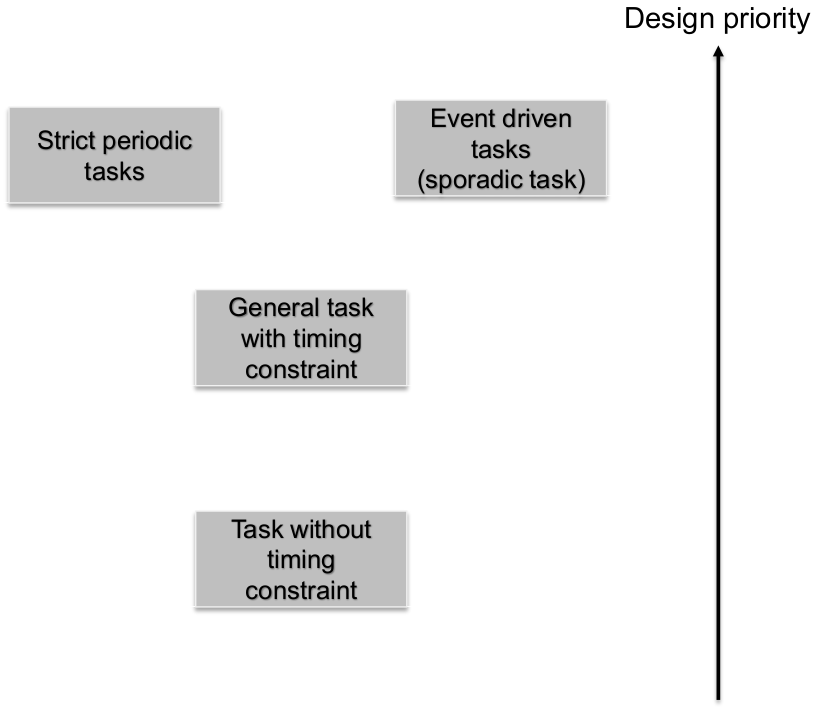
\includegraphics[width=\textwidth]{images/DesignStrategy/classify_tasks.png}
\end{minipage}


\subsubsection{Implementation without RTOS}
% \begin{minipage}[b]{0.6\textwidth}
The classification leads to the implementation in three different areas: Timer-ISR, ISR and main.
First steps can and should be implemented and tested separately.
Especially to determine WCET.
Since the ISR influence each other, tests must be undertaken with both implementations.
Last Step is to test the whole software architecture concerning real time behavior.

% \end{minipage}
% \begin{minipage}{0.39\textwidth}
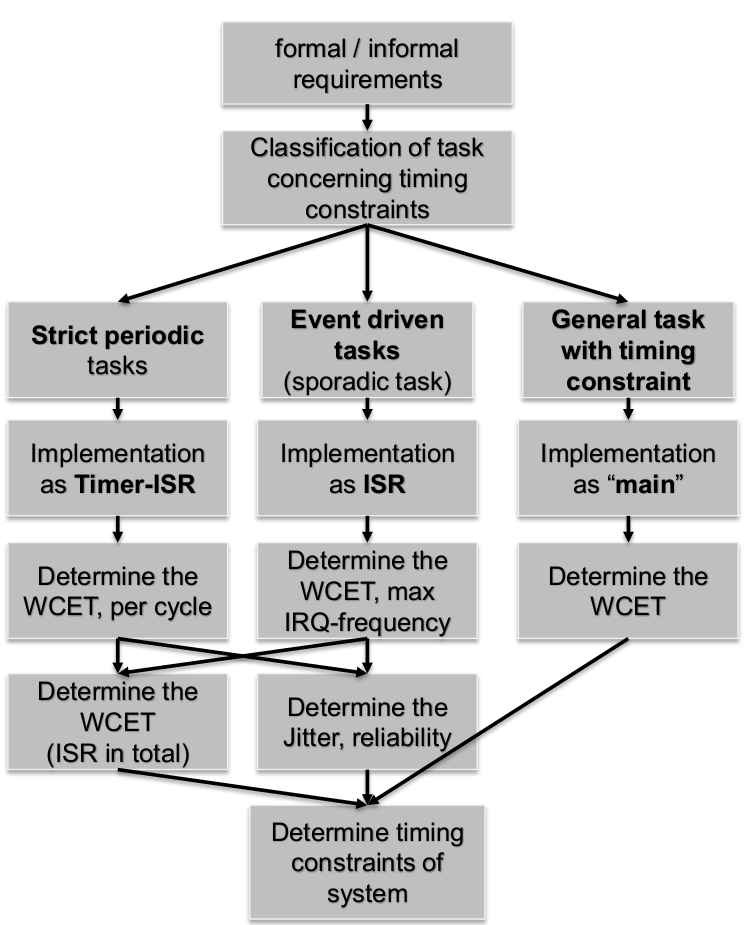
\includegraphics[width=0.4\textwidth]{images/DesignStrategy/task_implement_no_rtos.png}
% \end{minipage}

\subsubsection{Implementation with RTOS}
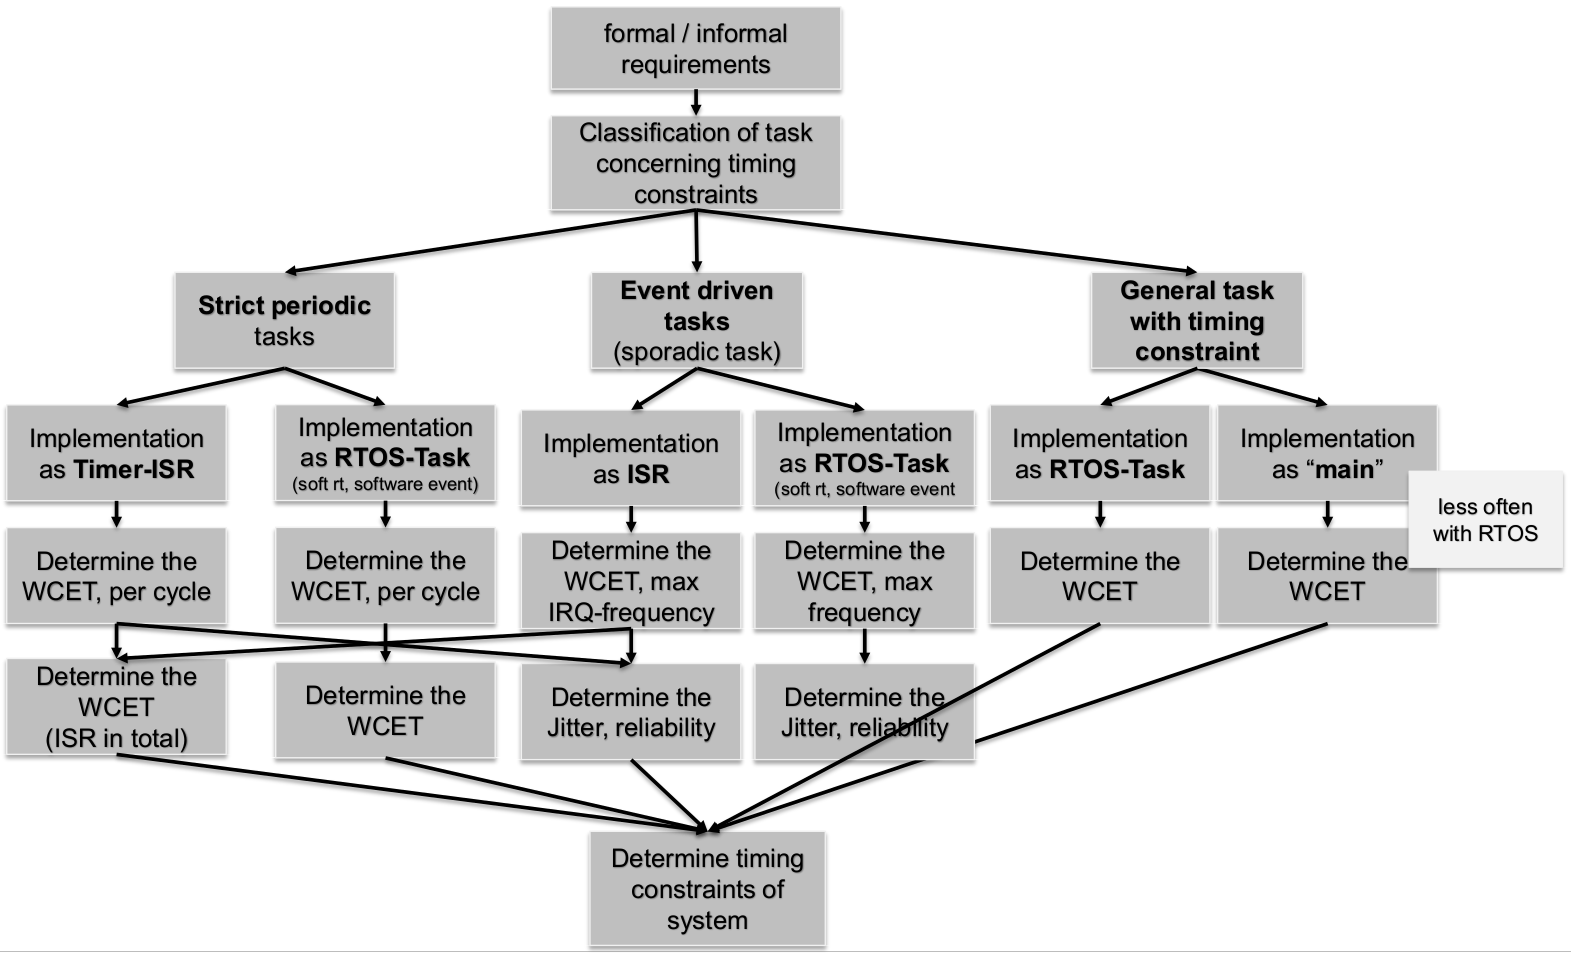
\includegraphics[width=0.9\textwidth]{images/DesignStrategy/task_implement_rtos.png}

\subsection{Approaches to define static Priorities for Tasks}
\subsubsection{Rate-Monotonic Approach: Short Code High priority}
The idea is that short ISR/tasks are executed fast.
Therefore, they block fo a very short time and execution is more guaranteed by priority.
\begin{itemize}
	\item Shortest ISR has highest priority
	\item Shortest flow/task has highest priority
\end{itemize}

\subsubsection{Important Code High Priority}
The idea is important ISR/tasks are executed fast.
\begin{itemize}
	\item Important ISR has highest priority
	\item Important task has highest priority
\end{itemize}

\subsubsection{Blended Approach}
Combination of RMA and ICH
\begin{itemize}
	\item Short task high priority
	\item Important ISR has high priority
\end{itemize}

\subsection{Interrupt Handling Concepts}
There are two main concepts how interrupt handling is implemented.

\begin{table}[h]
	\begin{tabularx}{\textwidth}{lXX}\hline
		Name        & Service Routine (ISR)                            & RTOS Task                                          \\\hline
		Description & Event code is executed mainly in the ISR         & ISR passes every executing code to RTOS task       \\
		Pros        & - Fastest execution                              & - RTOS support\newline - Interrupts fast available \\
		Cons        & - No or small RTOS support\newline - Blocks RTOS & - Slower execution, depended on RTOS scheduling    \\\hline
	\end{tabularx}
\end{table}

The approach of: \textbf{Interrupt handler in the RTOS task} is also called \textbf{software events} approach.
In a project they can also be combined.

\subsection{Prioritizing Interrupts, RTOS and Handling}
The real time system architecture can be influenced by defining the priority of the system timer of the RTOS!
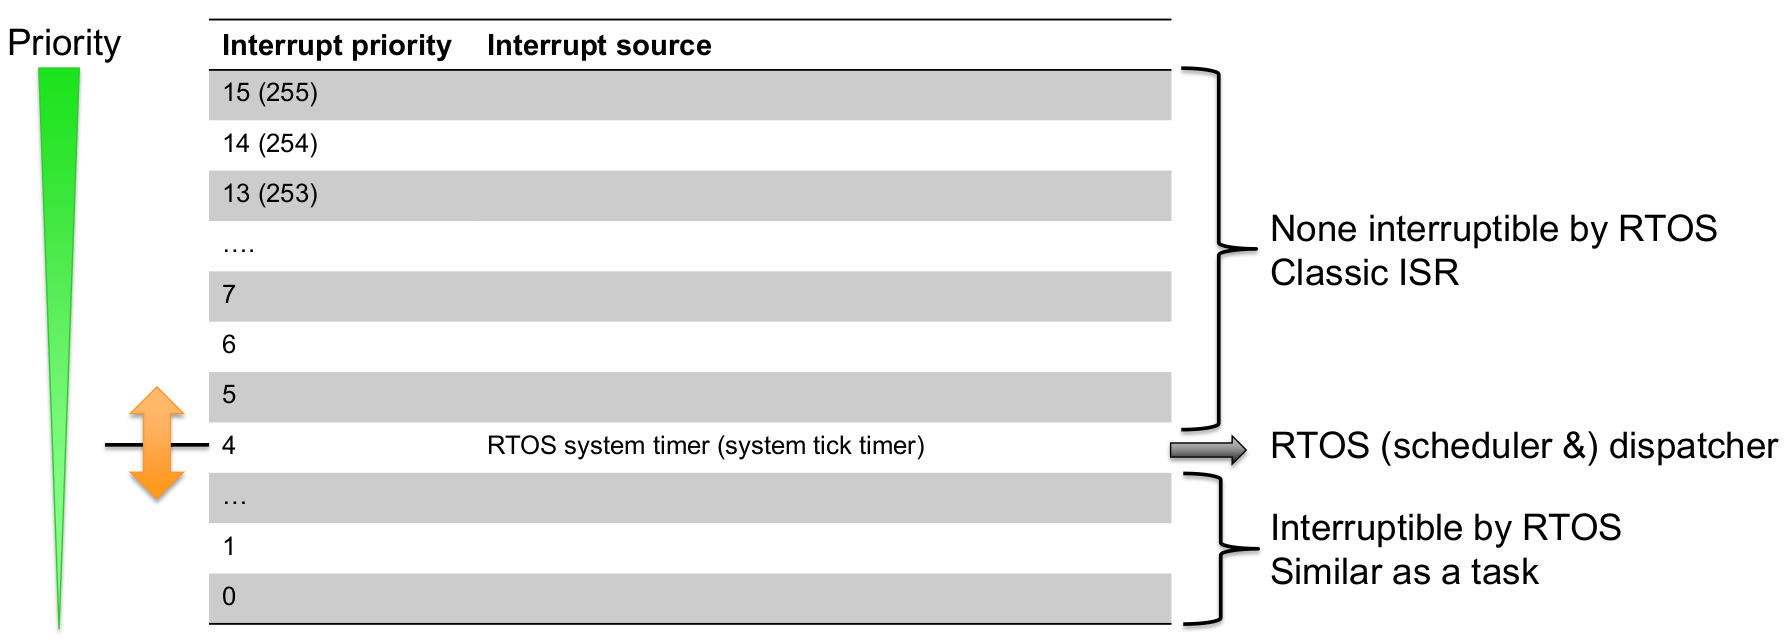
\includegraphics[width=\textwidth]{images/DesignStrategy/prio_interrupts.png}
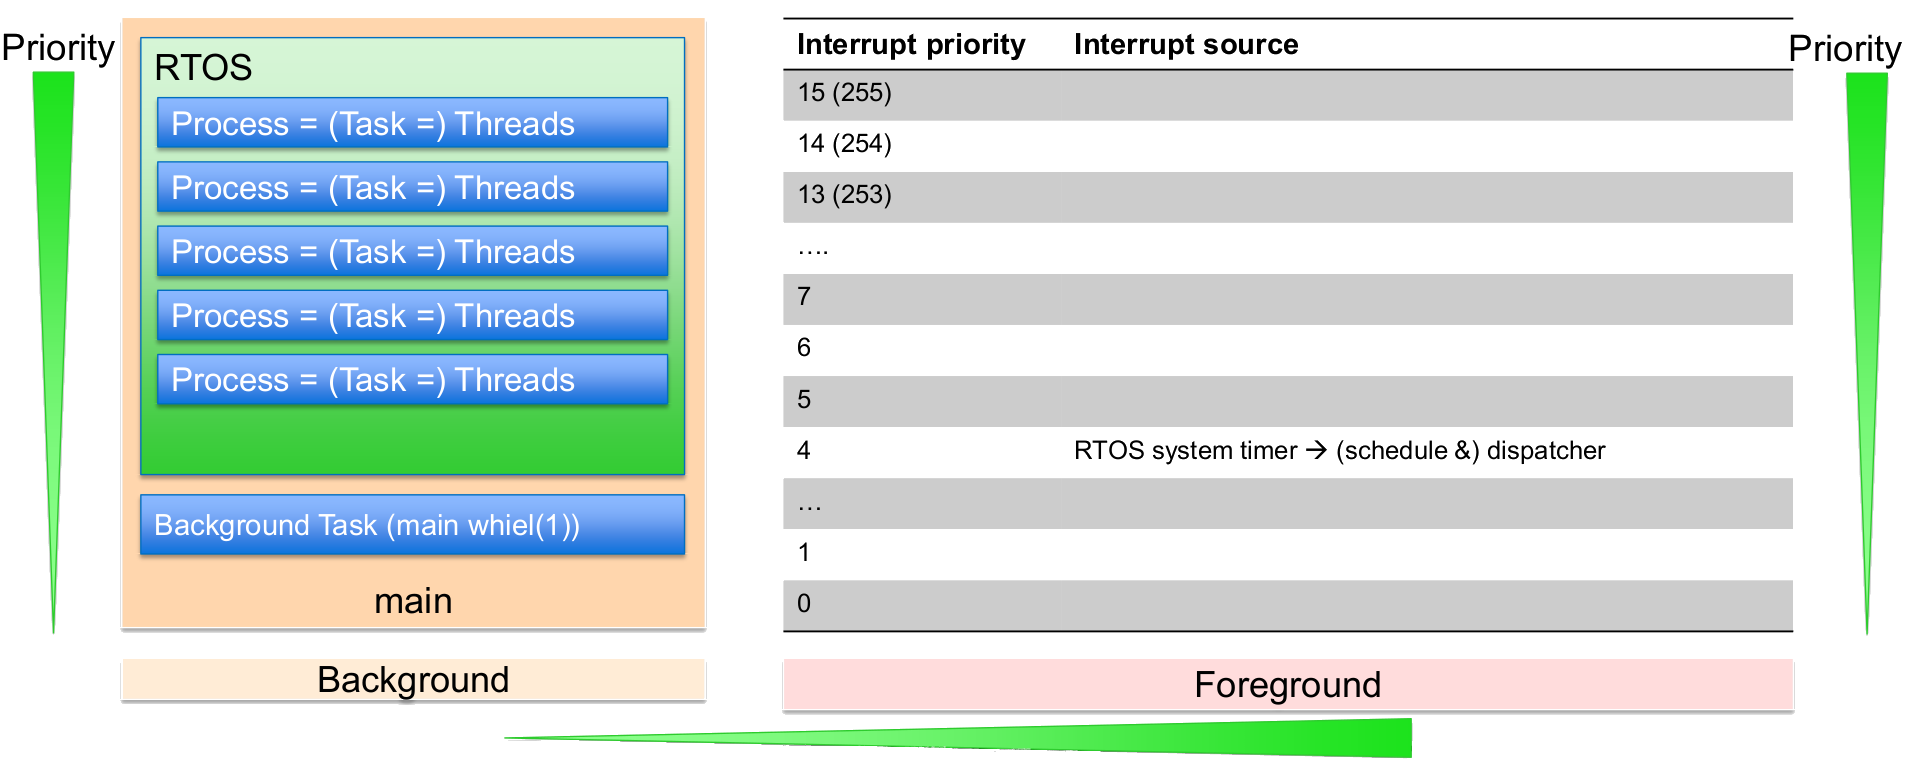
\includegraphics[width=\textwidth]{images/DesignStrategy/prio_interrupts_rtos_handling.png}
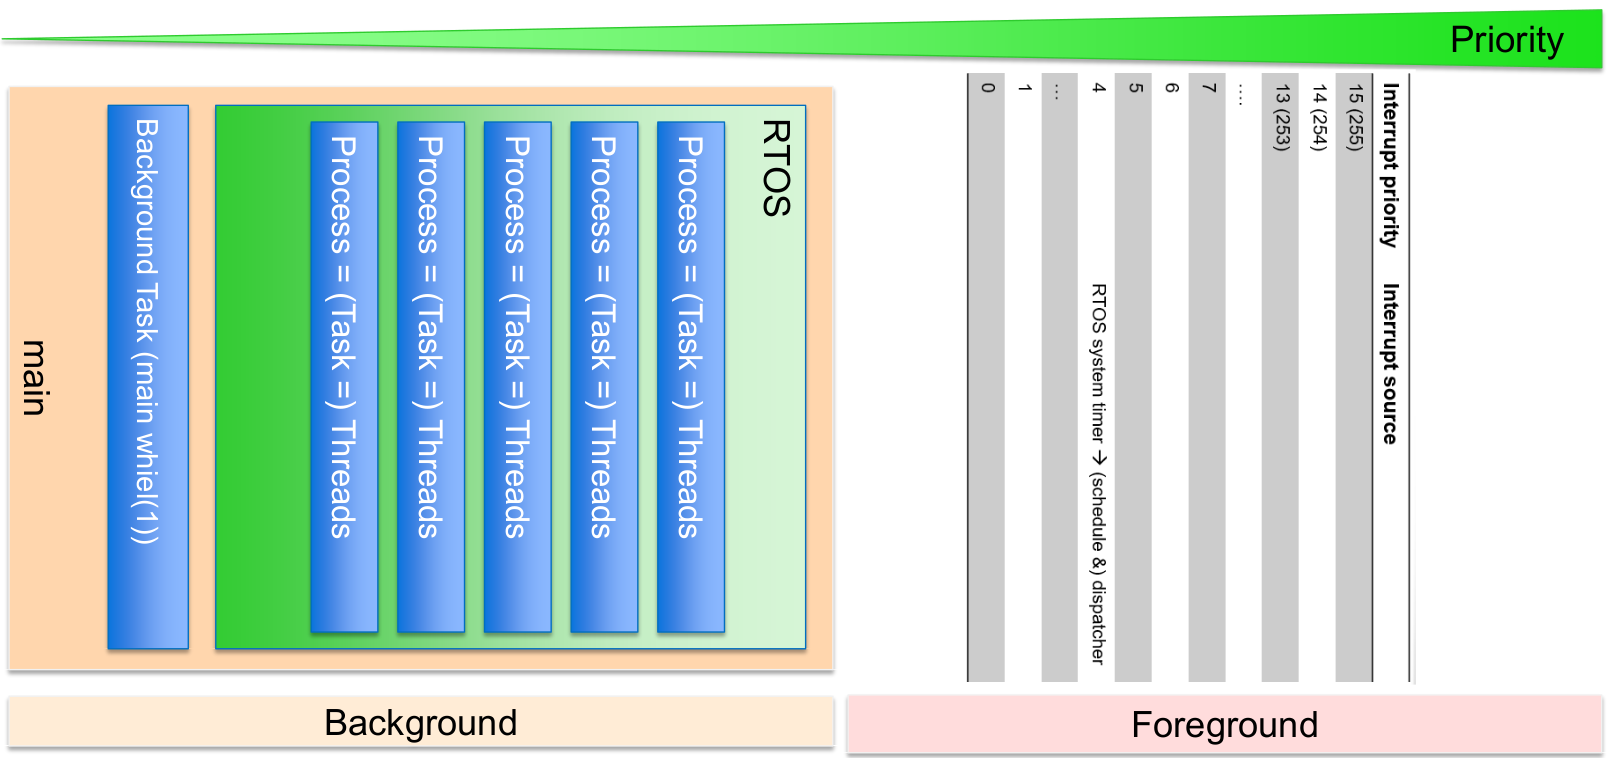
\includegraphics[width=\textwidth]{images/DesignStrategy/prio_interrupts_rtos_background.png}
\section{RTOS}
\subsection{POSIX Threads Programming}
\subsubsection{UNIX Process}
\begin{itemize}
    \item Heavyweight process (created by the operating system)
    \item Each process has its own protected address space.
    \item Processses are isolated so that they cannot inadvertently infringe on each other.
    \item Because of this enforces separation, communications between processes can take place only by using OS kernel services.
    \item Processes require a fair amount of overhead; they contain information about program resources and program execution state, including: Process ID, process group ID, user ID, and group ID; Environment; Program instructions; Registers; Stack; Heap; File descriptors; Signal actions; Shared libraries; Inter-process communication tools
\end{itemize}

\subsubsection{UNIX Thread}
\begin{itemize}
    \item A POSIX thread is a single flow of execution that runs within a process.
    \item \textbf{Threads use and exist within the process resources}
    \item \textbf{A thread uses the same address space as other threads of the same process}
    \item The main thread can create additional threads if it is so programmed.
          Thus, a process is virtually a collection of one or more threads.
    \item Threads are able to be scheduled by the operating system
    \item Independent stream of instructions that may run simultaneously to other streams of instructions
    \item Procedure that runs independently from its main program
    \item A thread maintains its own: Stack pointer; Registers; Scheduling properties; Set of pending and blocked signals; Thread specific data
    \item Concurrent programs are usually achieved with threads
\end{itemize}

\subsubsection{Process vs. Thread in UNIX}
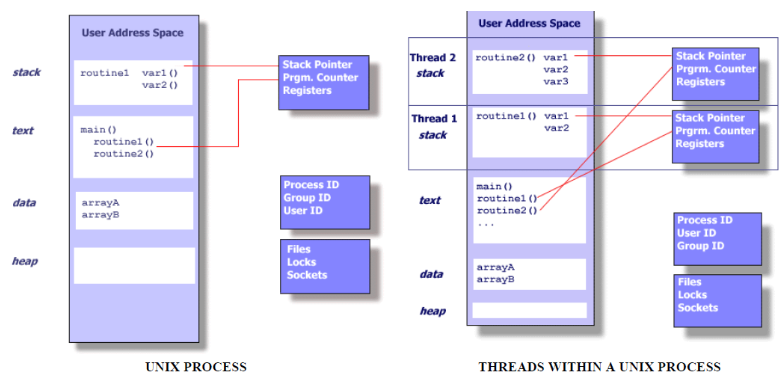
\includegraphics[width=12cm]{images/Concurrency/ProcessVsThread.png}

\subsection{What are POSIX Threads?}
\begin{itemize}
    \item For UNIX systems, a standardized C language threads programming interface has been specified by the \textbf{IEEE POSIX 1003.1c standard}.
    \item The short form of \textbf{POSIX threads} is \textbf{Pthreads} or \textbf{pthreads}.
    \item When compared to the cost of creating and managing a process, a thread can be created with much less operating system overhead
    \item Managing threads requires fewer system resources than managing processes
\end{itemize}

\subsection{Difference OS vs. RTOS}
A general purpose OS is system software that manages user applications and the hardware resources of a computer, defining rules and programming interfaces that allow a program to request OS services and interact with the rest of the system.
RTOS is an OS with many services commonly found in general-purpose OSs, such as multitasking, priority, task preemption, resource sharing, and intertask communication.
An RTOS is more than a general-purpose OS. An RTOS, with specialized scheduling algorithms, is intended to run real-time applications with soft and/or hard deadlines.
Thus, the key characteristic of an RTOS is that its response time to an event should be deterministic (or predictable).
An RTOS provides reliable mechanisms, such as real-time signals, preemptive scheduling, and nonblocking interprocess communications, for enabling a deterministic response.
\begin{itemize}
    \item RTOS is started in main
    \item Foreground and background process are dominating the OS
    \item A flow is a process or thread because the memory is not strictly isolated
    \item There are no sub flows
\end{itemize}
% \begin{paracol}{2}
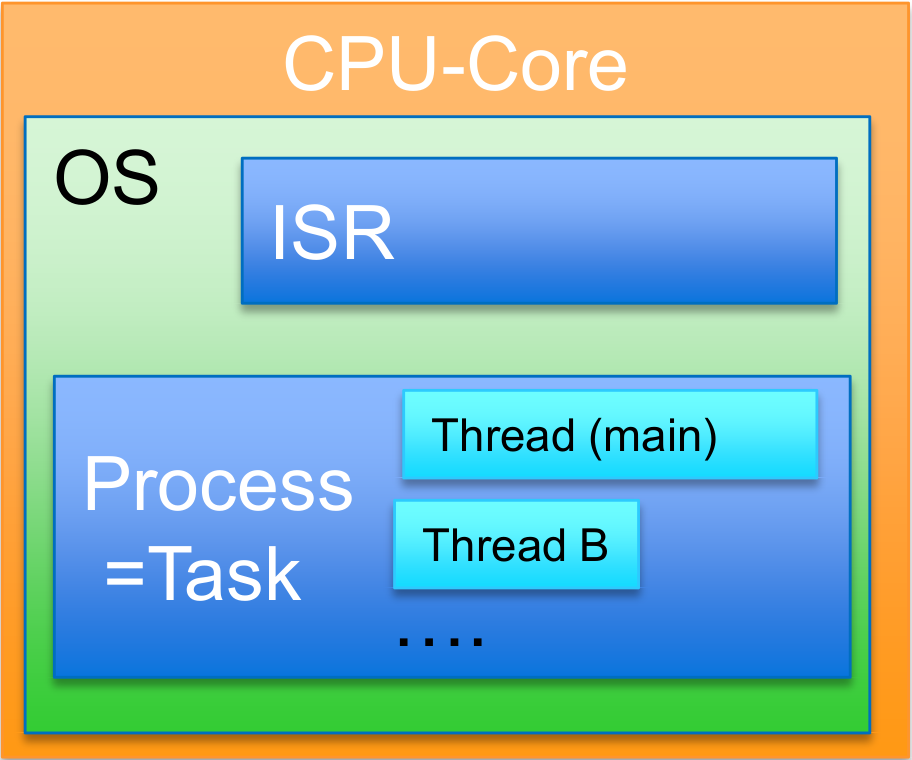
\includegraphics[width=0.25\textwidth]{images/Concurrency/os_process_thread.png}
% \switchcolumn
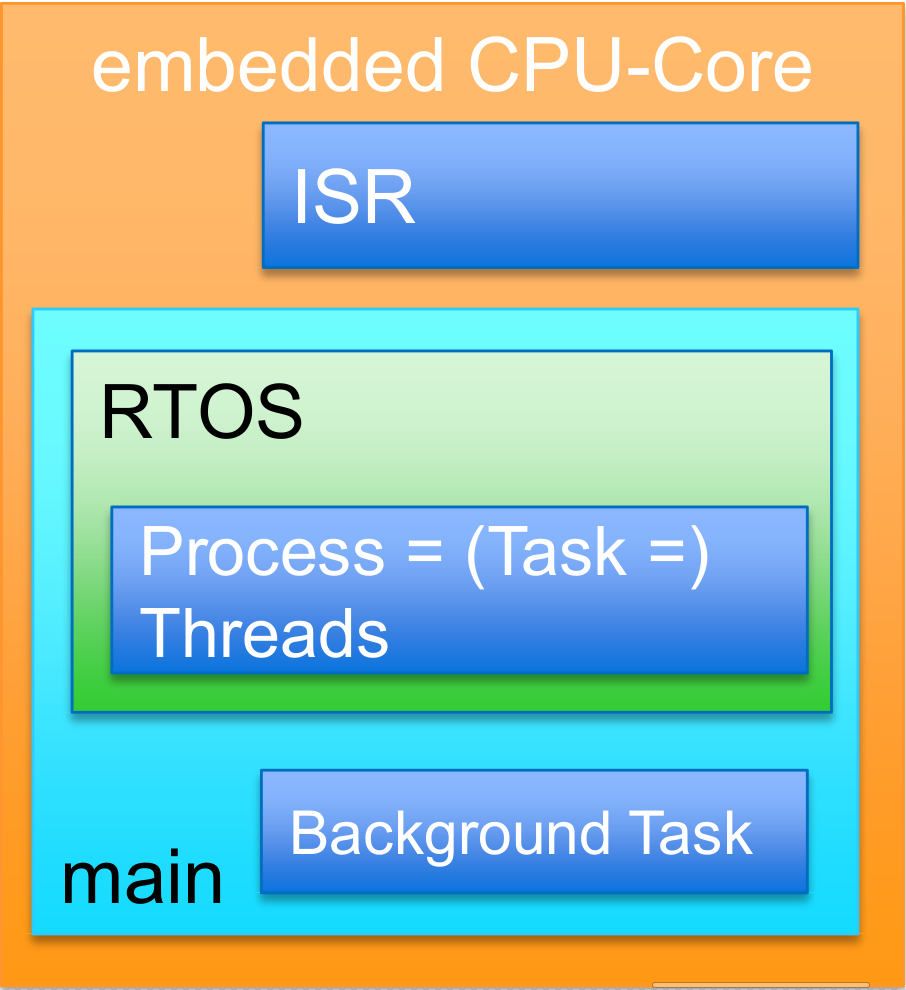
\includegraphics[width=0.25\textwidth]{images/Concurrency/rtos_process_thread.png}
% \end{paracol}

\subsection{System Structure}

\subsubsection{Scheduler and Dispatcher}
An RTOS needs at least one time basis.
This is often realized by one Timer with ISR!
The time basis defines how often a task can be dispatched.
This sets also some:
\begin{itemize}
    \item How high the overhead load for the CPU is
    \item Reaction time
    \item Timing constraints for WCE
\end{itemize}
The scheduler plans the next active Task according to priority and states of the task, which can be influenced by signals/events from ISR, main and tasks.\\
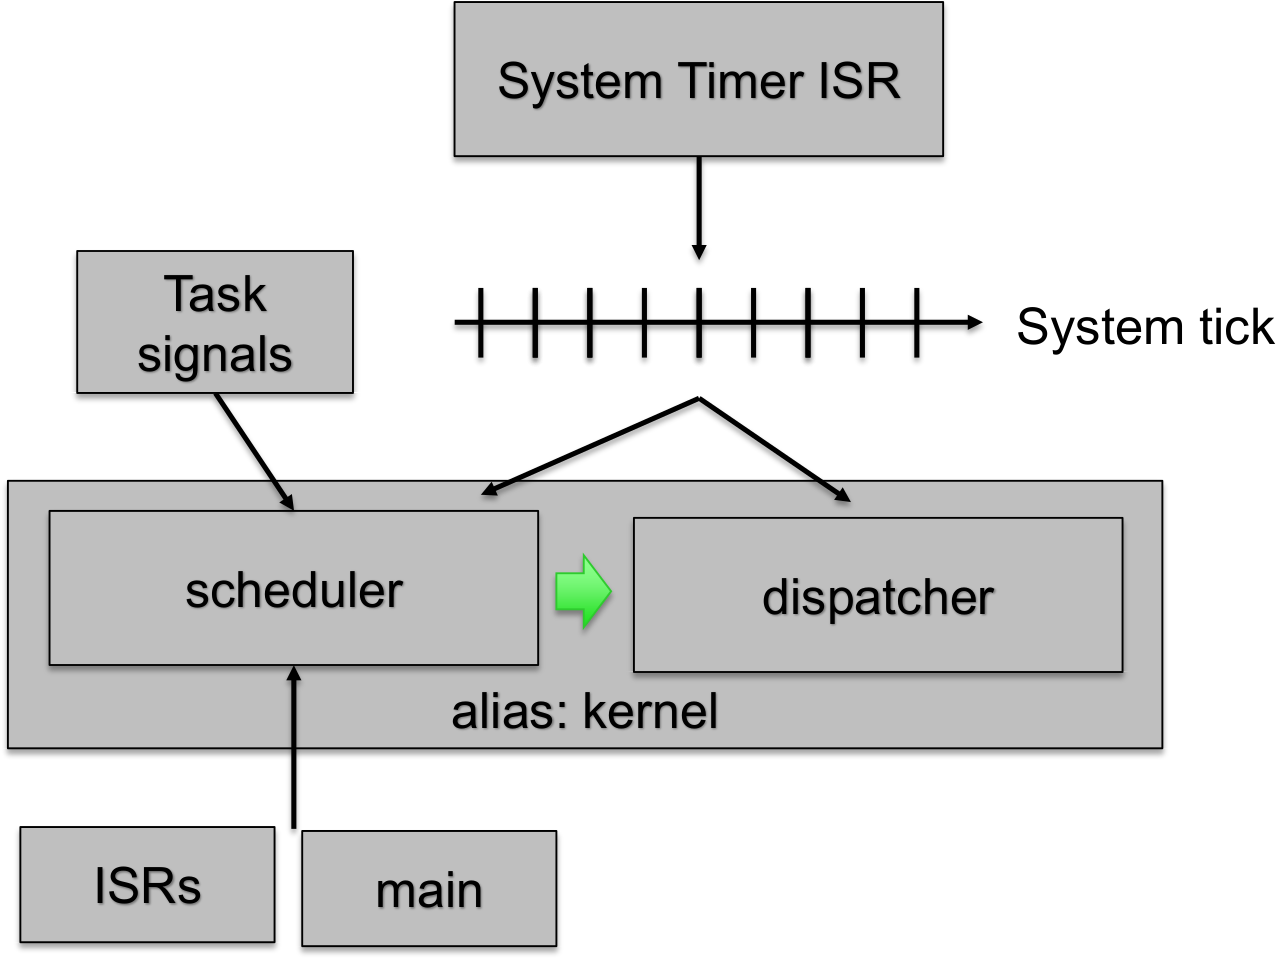
\includegraphics[width=0.5\textwidth]{images/RTOS/scheduler_dispatcher.png}

\subsubsection{Task States}
A task has different states, for instance:
\begin{itemize}
    \item Ready
    \item Running
    \item Blocked
    \item Sleeping
\end{itemize}
These terms are of the POSIX Standard, other RTOS may have different naming.\\
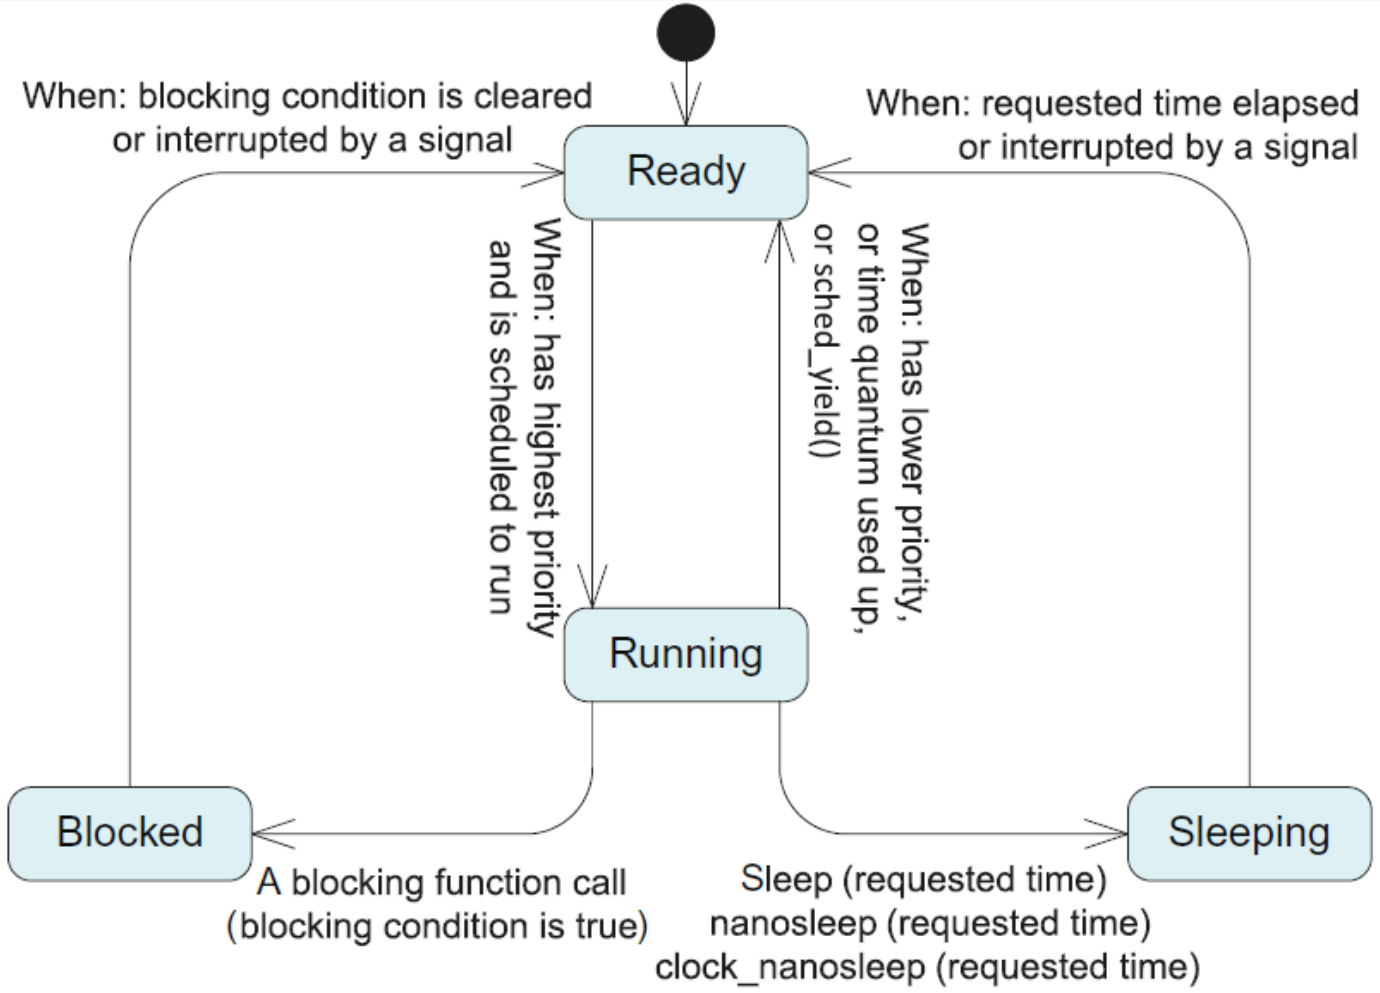
\includegraphics[width=0.5\textwidth]{images/RTOS/task_states_posix.png}

\section{FreeRTOS}
\begin{itemize}
    \item Developed and maintaned by Real Time Engineers Ltd.
    \item Supports 23 microcontroller architectures
    \item Small footprint (4.3Kbytes on an ARM7)
    \item Written in C
    \item Preemptive tasks
    \item Unlimited number of tasks and priorities
    \item Implements queues, binary/counting semaphores and mutexes
\end{itemize}

\subsection{Tasks}

\subsubsection{Task States}
\begin{minipage}{0.6\textwidth}
    \begin{description}
        \item[Running] When a task is actually executing it is said to be in the Running state.
              It is currently utilising the processor.
        \item[Ready] Ready tasks are those that are able to execute (they are not in the Blocked or Supsended state) but are not currently executing because a different tas of equal or higher priority is already in the Running State.
        \item[Blocked] A task is said to be in the Blocked state if it is currently waiting for either a temporal or external event.
              For example, if a task call \texttt{vTaskDelay()} it will block until the delay period is expired - a temporal event.
              Tasks can also block to wait for a queue, semaphore, event groupt, notification or semaphore event.
        \item[Suspended] Like tasks that are in the Blocked state, tasks in the Suspended state cannot be selected to enter the Running state, but tasks in the Suspended state do not have a time out.
              Instead, tasks only enter or exit the Suspended state when explicitly commanded to do so through the \texttt{vTaskSuspend()} and \texttt{xTaskResume()} API calls respectively.
    \end{description}
\end{minipage}
\begin{minipage}{0.4\textwidth}
    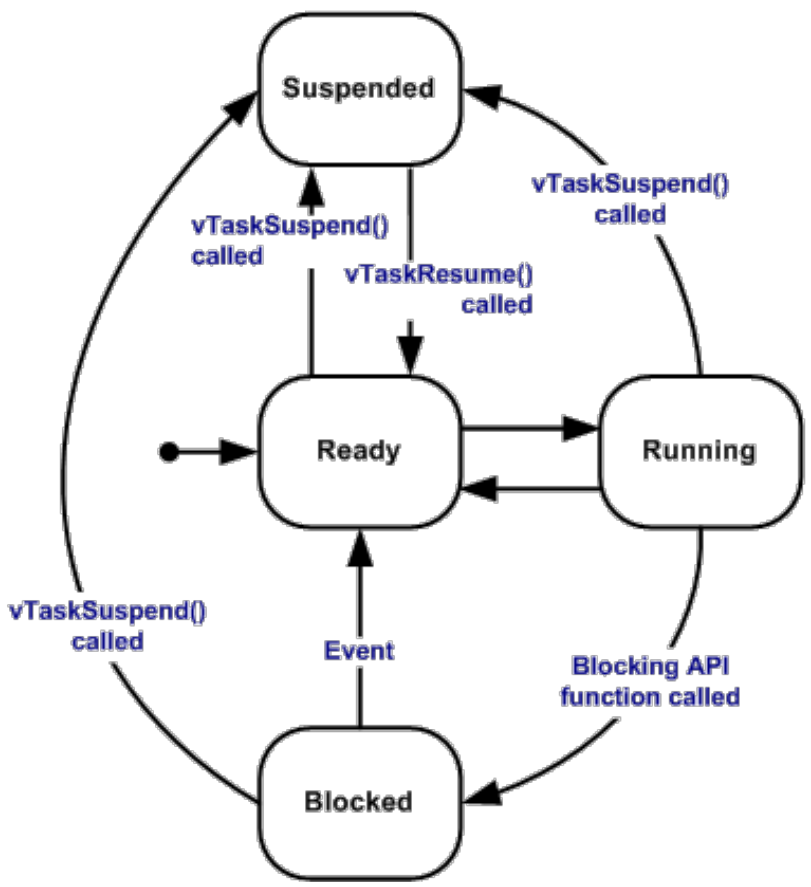
\includegraphics[width=1\textwidth]{images/RTOS/task_states_freertos.png}
\end{minipage}


\subsubsection{Task creation}
% \columnratio{0.5}
% \begin{paracol}{2}
\lstinputlisting[style=C, lastline=8]{snippets/FreeRTOS/task_creation.c}
% \switchcolumn
\lstinputlisting[style=C, firstline=10]{snippets/FreeRTOS/task_creation.c}
% \end{paracol}

\subsection{Communication}
\subsubsection{Pipes}
In FreeRTOS pipes are called Stream Buffers or Message Buffers

\subsubsection{Queues}
\lstinputlisting[style=C]{snippets/FreeRTOS/queue_functions.c}


\subsection{Resource Sharing}

\subsubsection{Semaphores}
\lstinputlisting[style=C]{snippets/FreeRTOS/semaphore_functions.c}

\subsubsection{Mutexes}
\lstinputlisting[style=C]{snippets/FreeRTOS/mutex_functions.c}

\subsubsection{Issue Solving in FreeRTOS}
Only supports priority inheritance (enable it in FreeRTOSConfig.h).
Further recommendation: Implement a tas with queue, \textbf{FreeRTOS Gatekeeper Task}.
% \section{Model Driven Development (MDD)}
\subsection{Modellierung eines Embedded Systems}

\textbf{Model Driven Approach (MDA)}
\begin{itemize}
	\item Modelle werden als Werkzeuge der Dokumentation angesehen. Dadurch wird unter Umständen dasselbe zweimal beschrieben (als Code und als Diagramm)

	\item Ziel ist es aus formalen Modellen lauffähige Software zu erzeugen. Bei State Machines ist dies durch Statecharts der Automaten vollständig möglich.
\end{itemize}

\textbf{Agile Softwareentwicklung}\\
Agile Softwareentwicklung ist der Oberbegriff für den Einsatz von Agilität (flink, beweglich) in der Softwareentwicklung.
\begin{itemize}
	\item Eher offen für Änderungen als starres Festhalten an Plänen
	\item Eher Menschen und Kommunikation als Prozesse und Tools
	\item Eher "`darüber miteinander reden"' als "`gegeneinander schreiben"'
	\item Eher Vertrauen als Kontrolle
	\item Eher "`Best Practices"' aus Erfahrung als verordnete Vorgaben
	\item Eher Angemessenheit als Extremismus
	\item \textbf{Aber: keine Anarchie!}
\end{itemize}

\textbf{Model Driven Development (MDD)}\\
Bei der modellbasierten Entwicklung kommen in allen Entwicklungsphasen durchgängig Modelle zur Anwendung.

\begin{multicols}{2}
	\begin{itemize}
		\item UML:
		      \begin{itemize}
			      \item Aktivitätsdiagramm
			      \item Sequenzdiagramm
			      \item Zustandsdiagramm (Statecharts)
			      \item Klassendiagramm
			      \item Use Case Diagramm
			      \item Verteilungsdiagramme (Deployment Diagram)
		      \end{itemize}
		\item Matlab/Simulink
		\item Petrinetze
		\item plus evtl. weitere
	\end{itemize}
	\vfill\null
	\columnbreak

	\textbf{Generelles Vorgehen bei der Modellierung:}
	\begin{enumerate}
		\item Systemgrenze definieren (statischer Aspekt)
		\item Systemprozesse finden (statischer Aspekt)
		\item Verteilung festlegen (statischer Aspekt)
		\item Systemprozesse detaillieren (dynamischer Aspekt)
	\end{enumerate}

	\textbf{Klassifizierung von Modellierungstechniken}\\
	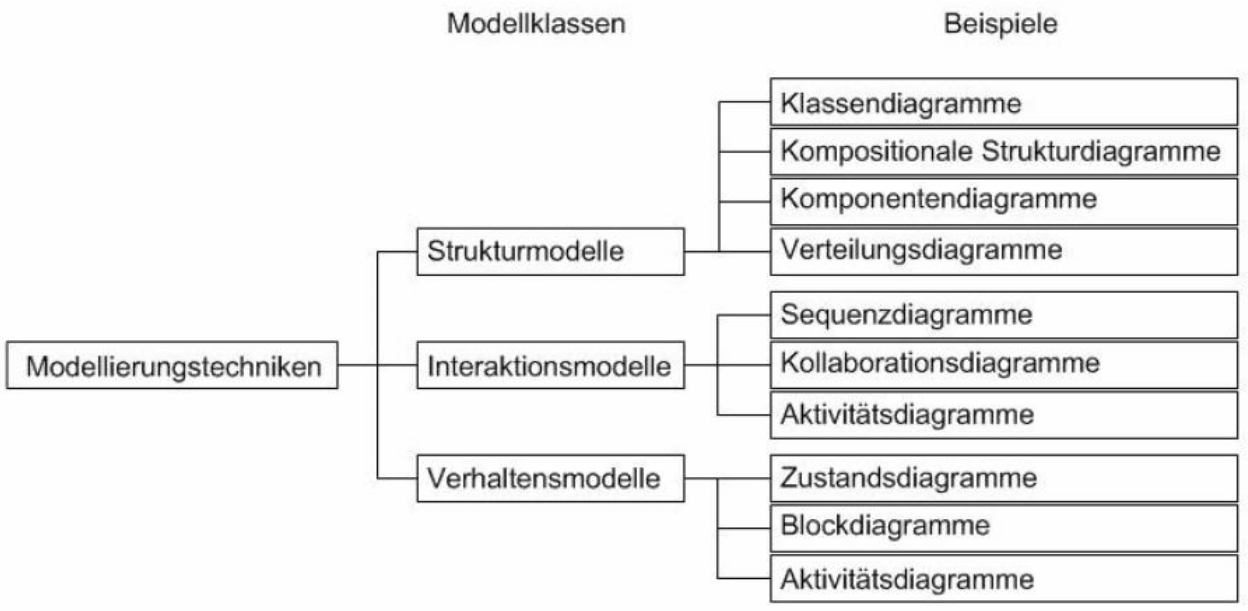
\includegraphics[width=\linewidth]{./images/Modellierung/klassifizierungModellierungstechniken}
	Wir beschäftigen uns in diesem Modul prioritär mit Interaktions- und Verhaltensmodellen, d.h. mit den dynamischen Aspekten.
\end{multicols}


\subsection{Systemgrenze definieren und Systemprozesse finden}
\subsubsection{Systemgrenze definieren}
Das wichtigste und allererste bei sämtlichen Systemen ist die Festlegung der Systemgrenze (system boundary) mittels Kontextdiagramm (\textbf{Use Case} oder auch \textbf{Sequenzdiagramm}).
\begin{itemize}
	\item Was macht das System, d.h was liegt innerhalb der Systemgrenze
	\item Mit welchen Teilen ausserhalb des Systems kommuniziert das System
	\item Welches sind die Schnittstellen zu den Nachbarsystemen
\end{itemize}

\subsubsection{Systemprozesse finden}
\begin{multicols}{2}
	Die Aufteilung in Hardware und Software sollte erst nach der Analyse der grundlegenden Anforderungen erfolgen. RTE-Systeme bestehen häufig nur aus einem einzigen Systemprozess, speziell wenn das System im Prinzip 'nur' ein Regler ist. Dieser Schritt ist in der Analysephase. Wenn hier von Prozessen die Rede ist, bedeutet das nicht ein Betriebssystem-Prozess. Wichtig ist, dass es nicht zuviele Funktionsblöcke gibt (nicht ins Detail gehen). \\
	Bei Systemen, bei denen die Grenzen durch Nachrichtenflüsse charakterisiert werden können, eignen sich \textbf{Sequenzdiagramme} zur Kontextbeschreibung.\\
	\vfill\null
	\columnbreak
	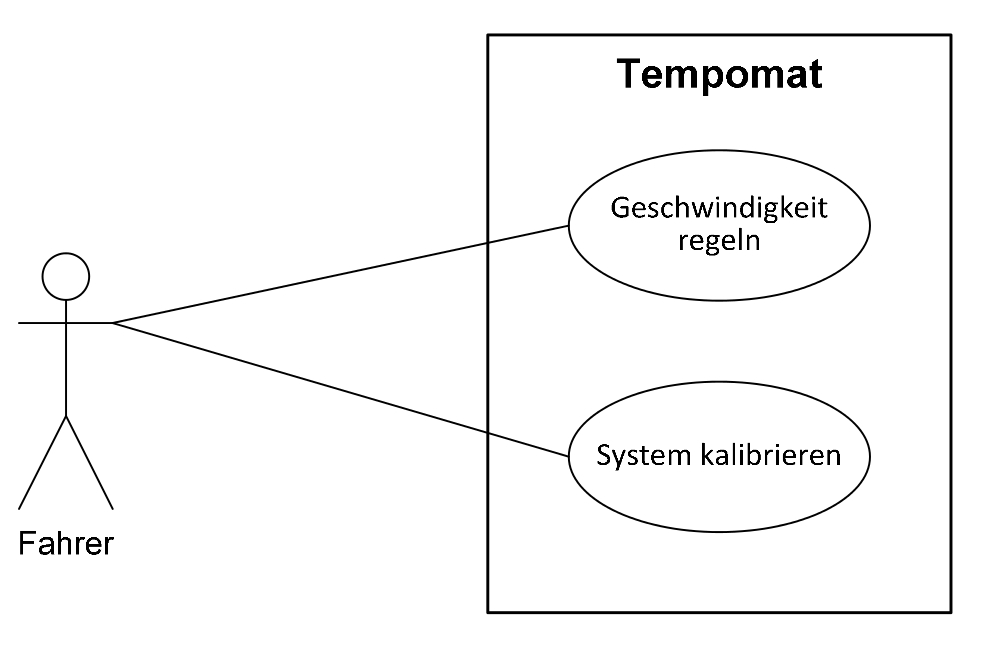
\includegraphics[height=6cm]{images/Modellierung/Systemgrenze}
\end{multicols}

\subsection{Verteilung festlegen}
Bei Embedded Systems werden häufig mehrere Rechnersysteme verwendet um die Aufgaben zu erledigen. Diese liegen meistens geografisch (cm bis km) verteilt und sind mit einem Kommunikationskanal verbunden. Diese Systeme heissen Verteilte Systeme (\textbf{Distributed Systems}). IoT-Systeme sind per Definition Verteilte Systeme.\\
Zur Darstellung eignet sich in UML das Verteilungsdiagramm (\textbf{Deployment Diagram}).

\subsubsection{Verteilungsdiagramm (Deployment Diagram)}
\begin{multicols}{2}
	\begin{itemize}
		\item Die Knoten werden zur Darstellung der geografischen Orte oder Subsysteme verwendet
		\item Die physikalischen Verbindungen zwischen den Knoten (Netzwerke, Kabel, Wireless, etc.) werden als Linien dargestellt.
		\item Die Knoten können auch hierarchisch aufgebaut sein.
	\end{itemize}
	\vfill\null
	\columnbreak
	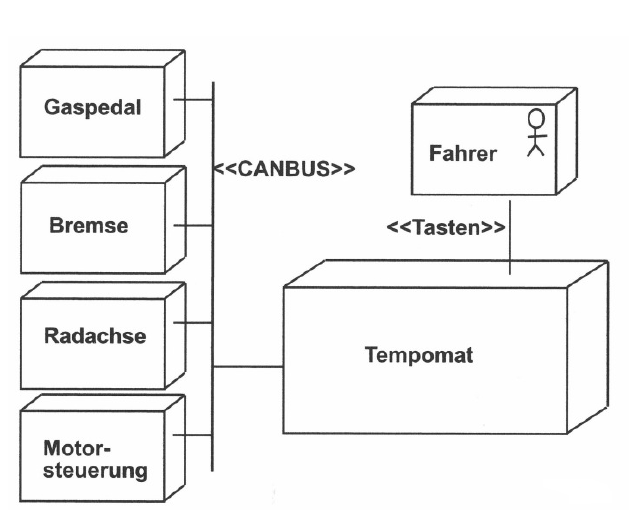
\includegraphics[height=6cm, width = 9cm,]{images/Modellierung/Verteilungsdiagramm}
\end{multicols}

\subsection{Systemprozesse Detaillieren}
Die gefundenen Systemprozesse müssen nun genauer spezifiziert werden. Dabei nicht detaillierter spezifizieren als sinnvoll. Jede weitere Detaillierung soll einen "`added value"' liefern.
Leitidee: Lieber weniger als mehr Details.

\subsubsection{Verschiedene Detaillierungsstufen}
\begin{itemize}[noitemsep,topsep=0pt]
	\item \textbf{Überblick: } z.B. in Form von normalem umgangssprachlichem Text. Diese Form sollte immer erstellt werden.
	\item \textbf{Normale Sicht: } Sie ist für den Systementwickler gedacht und enthält mehr Details.
\end{itemize}

Für die Detaillierung eignen sich: Umgangssprachlicher Text, Sequenzdiagramme, Aktivitätsdiagramme, Statecharts und Code (C, C++, ...).

\subsubsection{Sequenzdiagramme}
\begin{multicols}{2}
	\textbf{Zweck:}
	\begin{itemize}[noitemsep,topsep=0pt]
		\item Austausch von Meldungen zwischen Objekten innerhalb einer beschränkten Zeitdauer anzeigen
	\end{itemize}
	\vfill\null
	\columnbreak
	\textbf{Ideal:}
	\begin{itemize}[noitemsep,topsep=0pt]
		\item für kurze Zeitdauer mit einigen wenigen Objekten
		\item bei wenigen Verschachtelungen und Verzweigungen
	\end{itemize}
\end{multicols}

\begin{multicols}{2}
	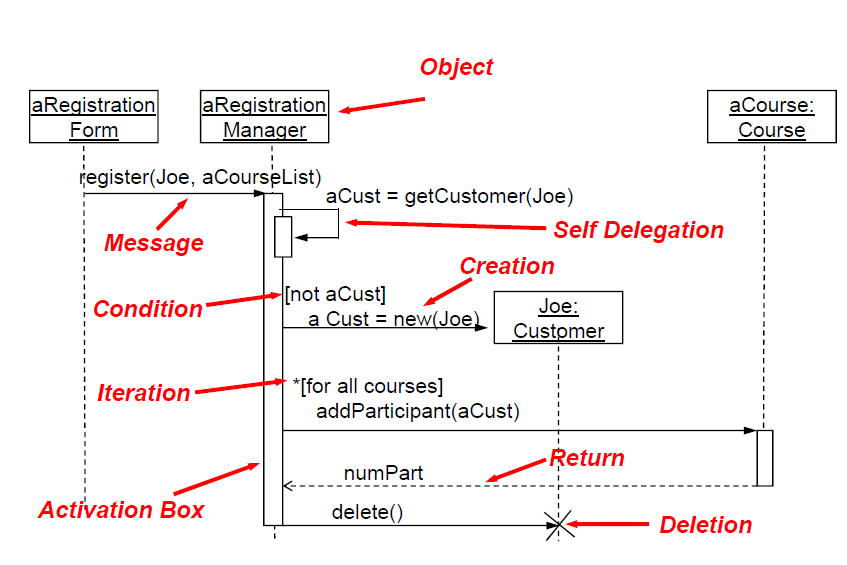
\includegraphics[width=\linewidth]{images/Modellierung/Sequenzdiagramm}
	\label{Bild1}
	\vfill\null
	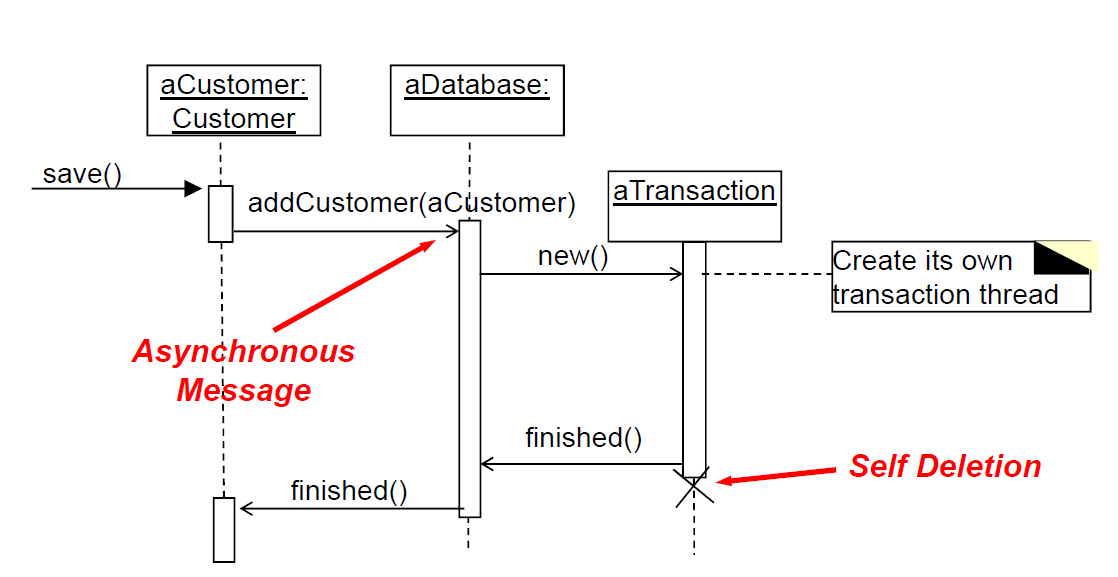
\includegraphics[width=\linewidth]{images/Modellierung/Sequenzdiagramm2}
	\label{Bild2}
\end{multicols}

\begin{multicols}{2}
	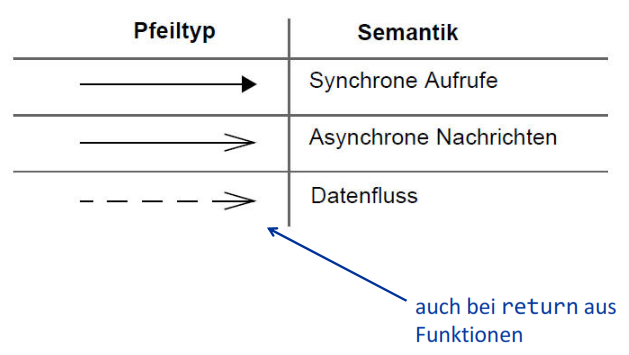
\includegraphics[width =\linewidth]{images/Modellierung/Pfeiltypen_Aktivitaetsdiagramm}
	\vfill\null
	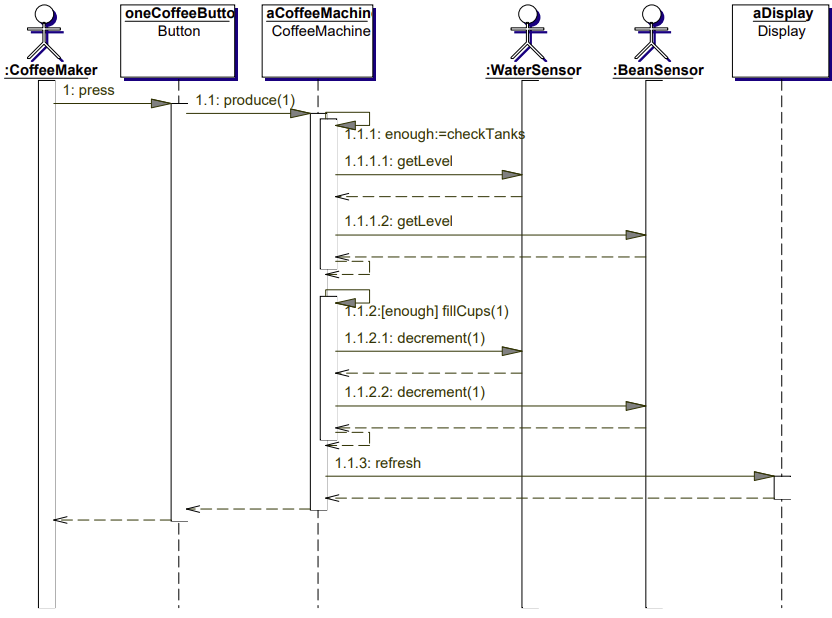
\includegraphics[height=5.5cm]{images/Modellierung/Aktivitaetsdiagramm_Beispiel_Kaffee.png}\\
	{\centering Beispiel: Kaffee Maschine}
\end{multicols}


\begin{multicols}{2}
	\textbf{Diagramm nicht überladen!}
	\vfill\null
	\columnbreak
	Wann einsetzen?
	\begin{itemize}[noitemsep,topsep=0pt]
		\item Use Case Analyse (Beschreibung von Szenario)
		\item Modellierung von Nachrichtenfluss
		\item SW-Design
		\item Implementation
	\end{itemize}
\end{multicols}

\newpage
\subsubsection{Kommunikationsdiagramm}
\begin{minipage}[][][t]{0.4\linewidth}
	Das Kommunikationsdiagramm zeigt dieselbe Information wie das Sequenzdiagramm. Der Schwerpunkt liegt aber
	nicht auf dem zeitlichen Ablauf, sondern auf dem Informationsfluss zwischen den Objekten.
\end{minipage}%
\begin{minipage}{0.6\linewidth}
	\begin{center}
		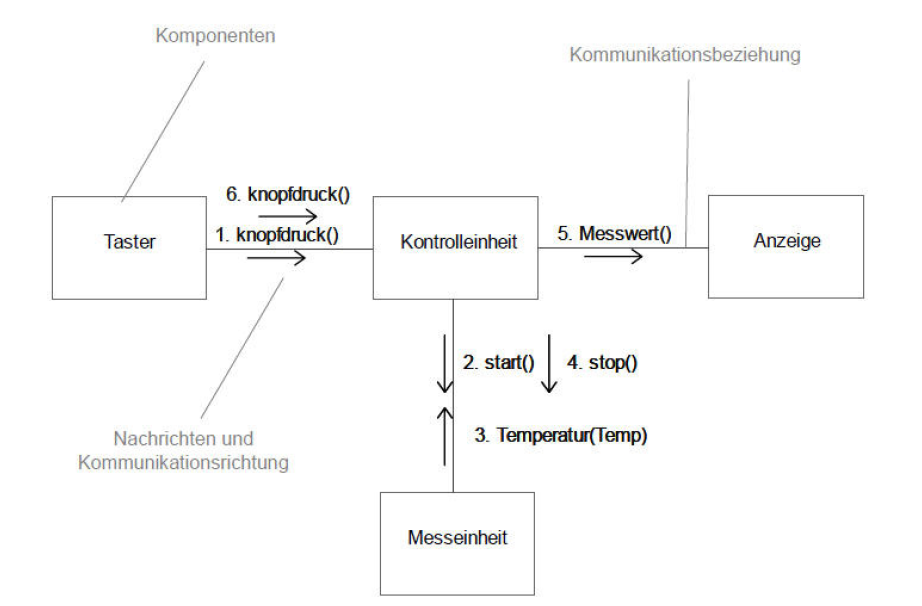
\includegraphics[width=0.8\linewidth]{images/Modellierung/Kommunikationsdiagramm}
	\end{center}
\end{minipage}

\subsubsection{Aktivitätsdiagramm}
\textbf{Wird gebraucht für:}
\begin{itemize}
	\item sequenzielle Abläufe
	\item Prozess- und Steuerfluss
	\item Auch für gleichzeitige Prozesse geeignet
	\item Weniger geeignet für komplexe logische Bedingungen (Wahrheitstabelle)
\end{itemize}

\begin{multicols}{2}
	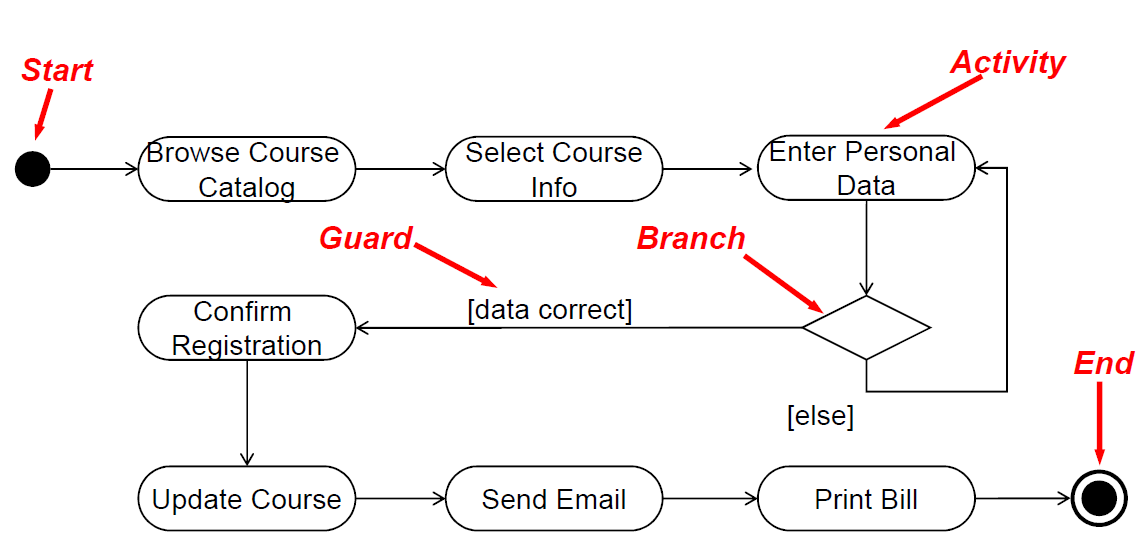
\includegraphics[width=\linewidth]{images/Modellierung/Aktivitaetsdiagramm1}
	\label{Bild3}
	\vfill\null
	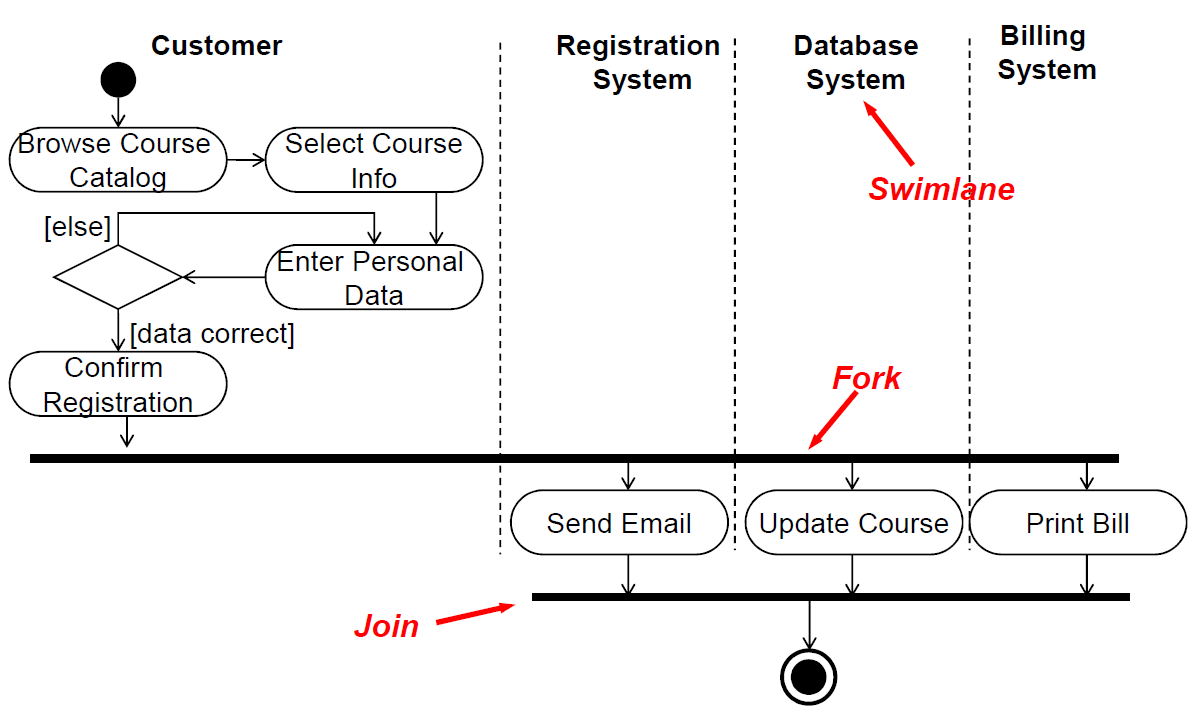
\includegraphics[width=\linewidth]{images/Modellierung/Aktivitaetsdiagramm2}
	\label{Bild4}
\end{multicols}

% \section{Zustandsbasierte Systeme}

\subsection{Finite State Machine (FSM)}
\subsubsection{Asynchrone vs. synchrone FSMs}
\begin{itemize}
  \item Bei (elektronisch implementierten) \textbf{asynchronen} FSMs führen geänderte Inputsignale direkt zu Zustands-\\änderungen. Sie sind deshalb "`schneller"', jedoch äusserst empfindlich auf Glitches und kaum testbar.
  \item Bei \textbf{synchronen} FSMs werden die Inputsignale nur zu diskreten Zeitpunkten betrachtet, diese Systeme sind getaktet.
  \item Softwareimplementationen sind eigentlich immer \textbf{synchron}, da die Rechner getaktet sind. Wenn die Inputsignale mittels Interrupts behandelt werden, ist darauf zu achten, dass die Interrupts nicht fälschlicherweise gesetzt werden (ist Aufgabe der Elektronik)
  \item Rein softwareseitig besteht die Problematik der \textbf{Asynchronizität} nicht
\end{itemize}

\subsubsection{Finite State Machine (FSM)}
\begin{minipage}{0.75\linewidth}
  \begin{itemize}
    \item Eine FSM befindet sich immer in einem definierten Zustand
    \item Die Inputs X bezeichnen üblicherweise Ereignisse (\textbf{Events})
    \item Die Outputs Y werden oft auch \textbf{Actions} genannt
    \item Eine FSM benötigt immer Speicherelemente zur Speicherung des \textbf{internen Zustands}
    \item In der Praxis sind zwei FSM-Varianten bekannt: \begin{itemize}
            \item der Mealy-Automat (Output abhängig vom Zustand \textbf{und} vom Input.)
            \item der Moore-Automat (Output nur vom Zustand abhängig.)
          \end{itemize}
  \end{itemize}
\end{minipage}
\begin{minipage}{0.25\linewidth}
  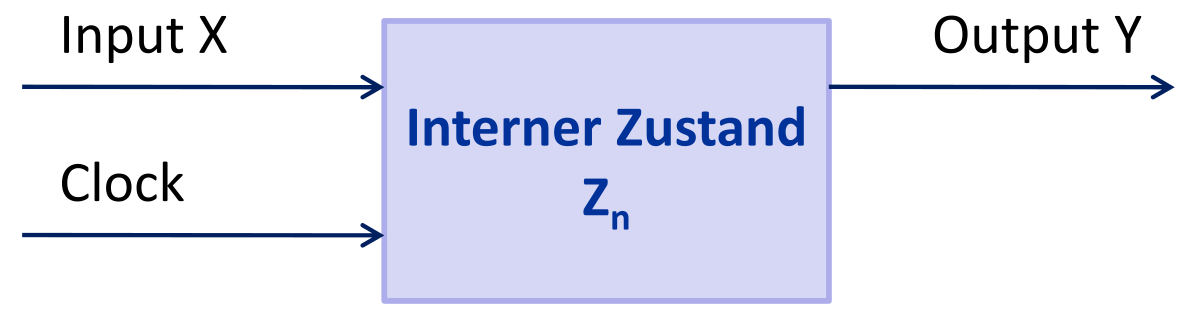
\includegraphics[width=\linewidth]{./images/FSM/fsm}
  \vfill\null
\end{minipage}

\subsubsection{Zustands-Ereignis-Diagramm (State-Event-Diagram)}
\begin{itemize}
  \item Die \textbf{Zustände} werden mit einem Kreis gekennzeichnet
  \item Die \textbf{Ereignisse} werden mit Pfeilen zwischen den Zuständen bezeichnet
        (\textbf{Transitionen})
  \item Die \textbf{Aktionen} werden entweder bei den Zuständen geschrieben oder bei den
        Transitionen (je nach Automatentyp)
  \item Die Ausführung einer \textbf{Transition} benötigt keine Zeit. Deshalb sind bei
        der Modellierung oft Zwischenzustände vorzusehen, z.B. "`Closing"', "`Starting
        up"', "`Booting"', etc.
\end{itemize}

\subsubsection{Mealy-Automat}
\begin{itemize}
  \item Der nächste Zustand $Z_{n+1}$ ist abhängig vom Input X und von $Z_n$:
        $Z_{n+1}=f(Z_n,X)$
  \item Der Output Y ist abhängig vom inneren Zustand $Z_n$ \textbf{und vom
          Input X}: $Y=g(Z_n, X)$
  \item Die \textbf{Actions} liegen deshalb bei den \textbf{Transitionen}
\end{itemize}

\subsubsection{Moore-Automat}
\begin{itemize}
  \item Der nächste Zustand $Z_{n+1}$ ist abhängig vom Input X und von $Z_n$:
        $Z_{n+1}=f(Z_n,X)$
  \item Der Output Y ist \textbf{nur} abhängig vom inneren Zustand $Z_n$: $Y=g(Z_n)$
  \item Die \textbf{Actions} liegen deshalb bei den \textbf{Zuständen}
\end{itemize}


\subsubsection{Zustandstabelle}

\renewcommand{\arraystretch}{1}
\begin{tabular}{|l|l|l|l|}
  \hline
  \textbf{Momentaner Zustand} & \textbf{Ereignis}  & \textbf{Nächster
  Zustand}                    & \textbf{Aktionen}                                            \\
  \hline
  AUS                         & EIN-Taste          & Hochlaufen       & Motor ausschalten    \\
                              &                    &                  & Kühlung ausschalten  \\&&&Grüne Lampe aus\\&&&Rote Lampe aus\\
  \hline
  Hochlaufen                  & Drehzahl\_erreicht & Drehzahl\_ok     & Motor einschalten    \\
                              & Signal             &                  & Kühlung einschalten  \\ \cline{2-3}
                              & AUS-Taste          & AUS              &                      \\\cline{2-3}
                              & Wasserkühlung      & Störung          &                      \\
                              & Störung            &                  &                      \\
  \hline
  Drehzahl\_ok                & Wasserkühlung      & Störung          & Grüne Lampe anzeigen \\
                              & Störung            &                  &                      \\ \cline{2-3}
                              & AUS-Taste          & AUS              &                      \\
  \hline
  Störung                     & RESET-Taste        & AUS              & Motor ausschalten    \\
                              &                    &                  & Kühlung ausschalten  \\&&&Rote Lampe anzeigen\\
  \hline
\end{tabular}
\renewcommand{\arraystretch}{1.8}

\subsubsection{Nachteile von Zustandsdiagrammen}
\begin{multicols}{2}
  \begin{itemize}
    \item Für einen Resetzustand muss von jedem State zum Resetstate eine Transition gezeichnet werden.
    \item Da Zustandsdiagramme flach sind (es gibt keine Hierarchie), werden sie bei
          praktisch relevanten Aufgaben schnell unübersichtlich
    \item In Zustandsdiagrammen kann keine zeitliche Parallelität modelliert werden
  \end{itemize}
  \vfill\null
  \columnbreak
  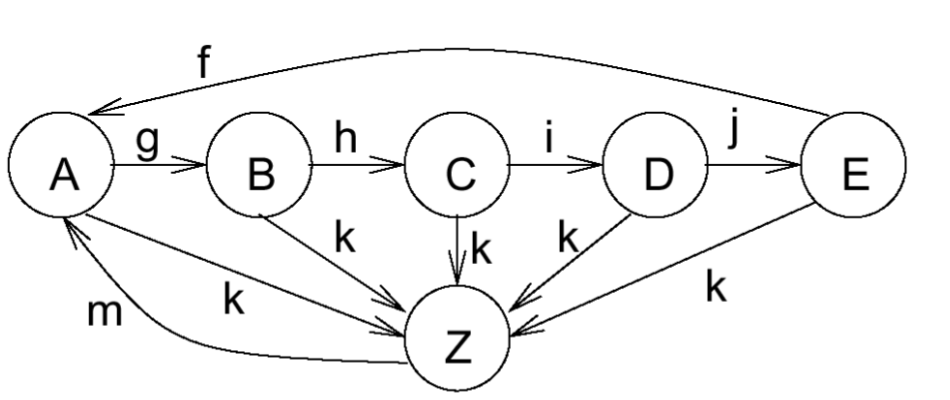
\includegraphics[width=0.9\linewidth]{images/FSM/reset_state}
\end{multicols}

\newcommand{\kreis}[1]{\unitlength1ex\begin{picture}(2.5,2.5)%
    \put(0.75,0.75){\circle{3.5}}\put(0.75,0.75){\makebox(0,0){#1}}\end{picture}}

\subsection{Statecharts von Harel}
\subsubsection{Elemente der Statechart}
\begin{tabular}{ll}
  $\bullet$  & Anfangszustand (initial pseudo state)                              \\
  $\diamond$ & Entscheidung (choice)                                              \\
  $\bullet$  & Kreuzung (junction)                                                \\
  $\times$   & Terminator (terminate pseudo state)                                \\
  \kreis{H}  & flache Historie (shallow history): History-Mechanismus merkt sich
  frühere Zustände                                                                \\
  \kreis{H*} & tiefe Historie (deep history): Deep History-Mechanismus merkt sich
  Zustände bis in die unterste Hierarchie                                         \\
  \kreis{}   & Eintrittspunkt (entry point)                                       \\
  $\otimes$  & Austrittspunkt (exit point)                                        \\
\end{tabular}
\pagebreak\newpage

\subsubsection{Modellierung von einfacher Hierarchie}
\begin{itemize}
  \item Hierarchie wird mit Hilfe von Superzuständen (superstates) eingeführt.
  \item Zustände, die andere Zustände enthalten, heissen Superzustände.
  \item Zustände, die in anderen Zuständen enthalten sind, heissen Unterzustände der Superzustände.
\end{itemize}
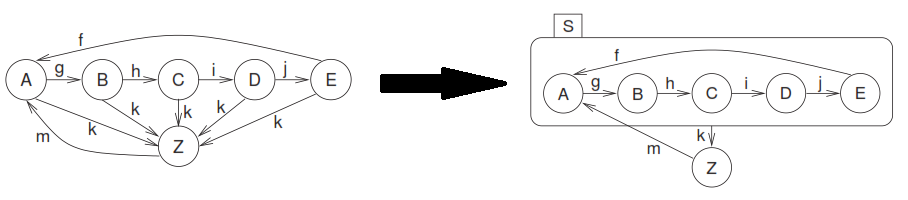
\includegraphics[width = 12cm]{images/FSM/Hierarchie}\\\\
Superzustand S beinhaltet die Zustände A, B, C, D und E. Angenommen, der Automat befindet sich in Zustand Z (wird auch als aktiver Zustand beschrieben). Wenn dann die Eingabe m am Automaten erfolgt, ist A der nächste Zustand. Wenn sich der Automat in Zustand S befindet und es gibt die Eingabe k, so ist Z der nächste Zustand, unabhängig davon, in welchem der Unterzustände A, B, C, D oder E sich der Automat tatsächlich befindet. In diesem Beispiel sind alle in S enthaltenen Zustände nicht-hierarchische Zustände. Im Allgemeinen könnten die Unterzustände von S selbst wieder Superzustände sein, die weitere Unterzustände enthalten.
\begin{itemize}
  \item Jeder Zustand, der nicht aus anderen Zuständen besteht, heisst Basiszustand.
  \item Superzustände S heissen ODER-Superzustände, wenn das System, das S enthält, sich zu jedem Zeitpunkt lediglich in einem einzigen Unterzustand von S befinden kann, solange es sich in S befindet.
\end{itemize}

\subsubsection{Modellierung von Hierarchie mit Default State (Standardzustand)}
\begin{multicols}{2}
  Der Standardzustand kann in Superzuständen verwendet werden, um anzuzeigen, welcher der Unterzustände betreten wird, wenn der Superzustand betreten wird.
  Dies wird mit einem kleinen ausgefüllten Kreis dargestellt.\\
  \vfill\null
  \columnbreak
  \begin{center}
    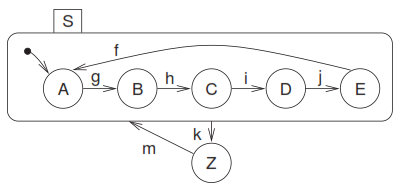
\includegraphics[width=0.6\linewidth]{images/FSM/Hierarchie_DefaultState}
  \end{center}
\end{multicols}

\subsubsection{Modellierung von Hierarchie mit History}
Mit Hilfe des History-Mechanismus ist es möglich, in den letzten Unterzustand zurückzukehren, der aktiv war, bevor der Superzustand verlassen wurde. Der History-Mechanismus wird durch den Buchstaben H in
einem Kreis dargestellt.\\
\begin{minipage}[hbt]{8cm}
  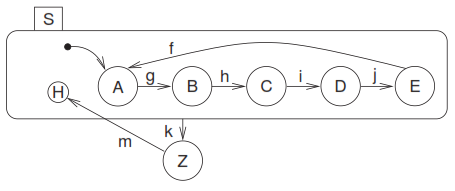
\includegraphics[width=6cm]{images/FSM/Hierarchie_History}
\end{minipage}
\begin{minipage}[hbt]{6cm}
  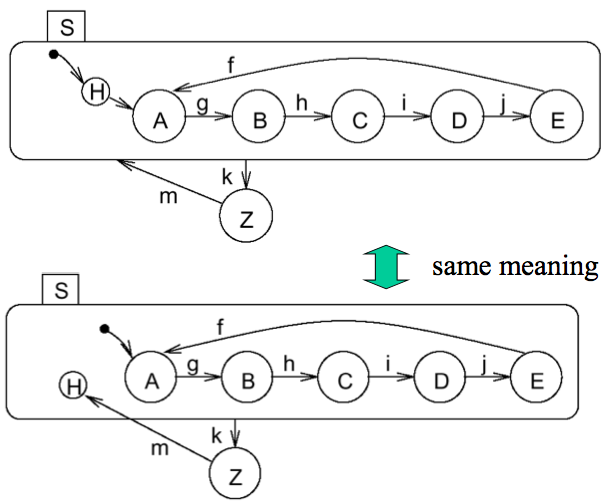
\includegraphics[width = 6cm]{images/FSM/history_default_state_mechanism}
\end{minipage}
\pagebreak\newpage

\subsubsection{Parallelität (UND-Superzustände)}
\begin{multicols}{2}
  Eine Spezifikationstechnik muss auch in der Lage sein, Nebenläufigkeit und Parallelität darzustellen. Zu diesem Zweck gibt es eine zweite Art von Superzuständen, die sogenannten UND-Superzustände.
  \begin{itemize}
    \item Superzustände S heissen UND-Superzustände, wenn das System, das S enthält, sich in allen Unterzuständen von S gleichzeitig befindet,
          solange es sich in S befindet.
  \end{itemize}
  \vfill\null
  \columnbreak
  \begin{center}
    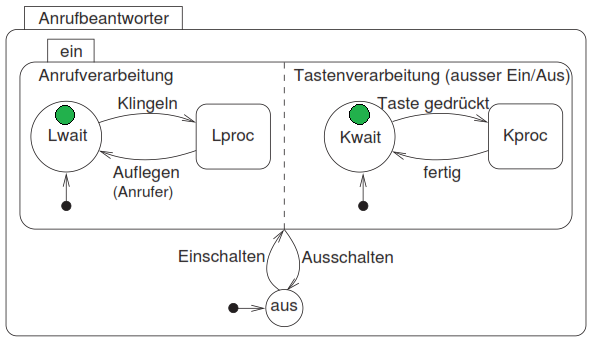
\includegraphics[width=0.8\linewidth]{images/FSM/AND_super_state}
  \end{center}
\end{multicols}

\subsubsection{Zeitbedingungen}
\begin{multicols}{2}
  Da es notwendig ist, in eingebetteten Systemen Zeitbedingungen zu modellieren, bieten Statecharts die sogenannten Timer an. Zeitbedingungen werden durch das gezackte Symbol dargestellt.\\
  Wenn das System für die im Timer angegebene Zeitdauer im Timer-Zustand war, wird ein Time-Out ausgelöst und das System verlässt diesen Zustand. Timer können auch hierarchisch verwendet werden.\\
  \vfill\null
  \begin{center}
    \columnbreak
    Timer bei einem Telefon-Beantworter:\\
    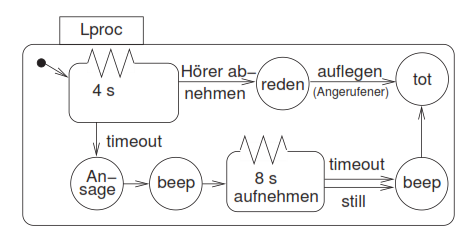
\includegraphics[width=8cm]{images/FSM/timer}
  \end{center}
\end{multicols}
\newpage
\subsubsection{Beispiel Alarmanlage}
\begin{itemize}
  \item \textbf{Aufgabenstellung:}\\In einem Haus sollen vier Fenster und eine Tür gegen Einbruch gesichert werden. Die einzelnen Fenster
        sind jeweils mit Glasbruchsensoren ausgestattet. Im Inneren des Hauses befindet sich ferner ein Bewegungsmelder, der die Eingangstür gegen Eindringlinge absichern soll. Der Alarm soll aktiviert werden, wenn
        ein Fenster zerstört wird oder wenn der Bewegungsmelder mindestens zwei Sekunden lang eine Bewegung
        meldet (die Verzögerung dient der Vermeidung von Fehlalarmen).\\
        Damit der rechtmässige Besitzer die Alarmanlage ein- und ausschalten kann, ohne sofort einen Alarm auszulösen, soll das Gerät vor dem Scharfstellen sowie vor dem Auslösen des Alarms eine Latenzzeit von 30
        Sekunden einhalten, in der man das Haus verlassen bzw. die Anlage deaktivieren kann.
  \item \textbf{Lösung:}\\ 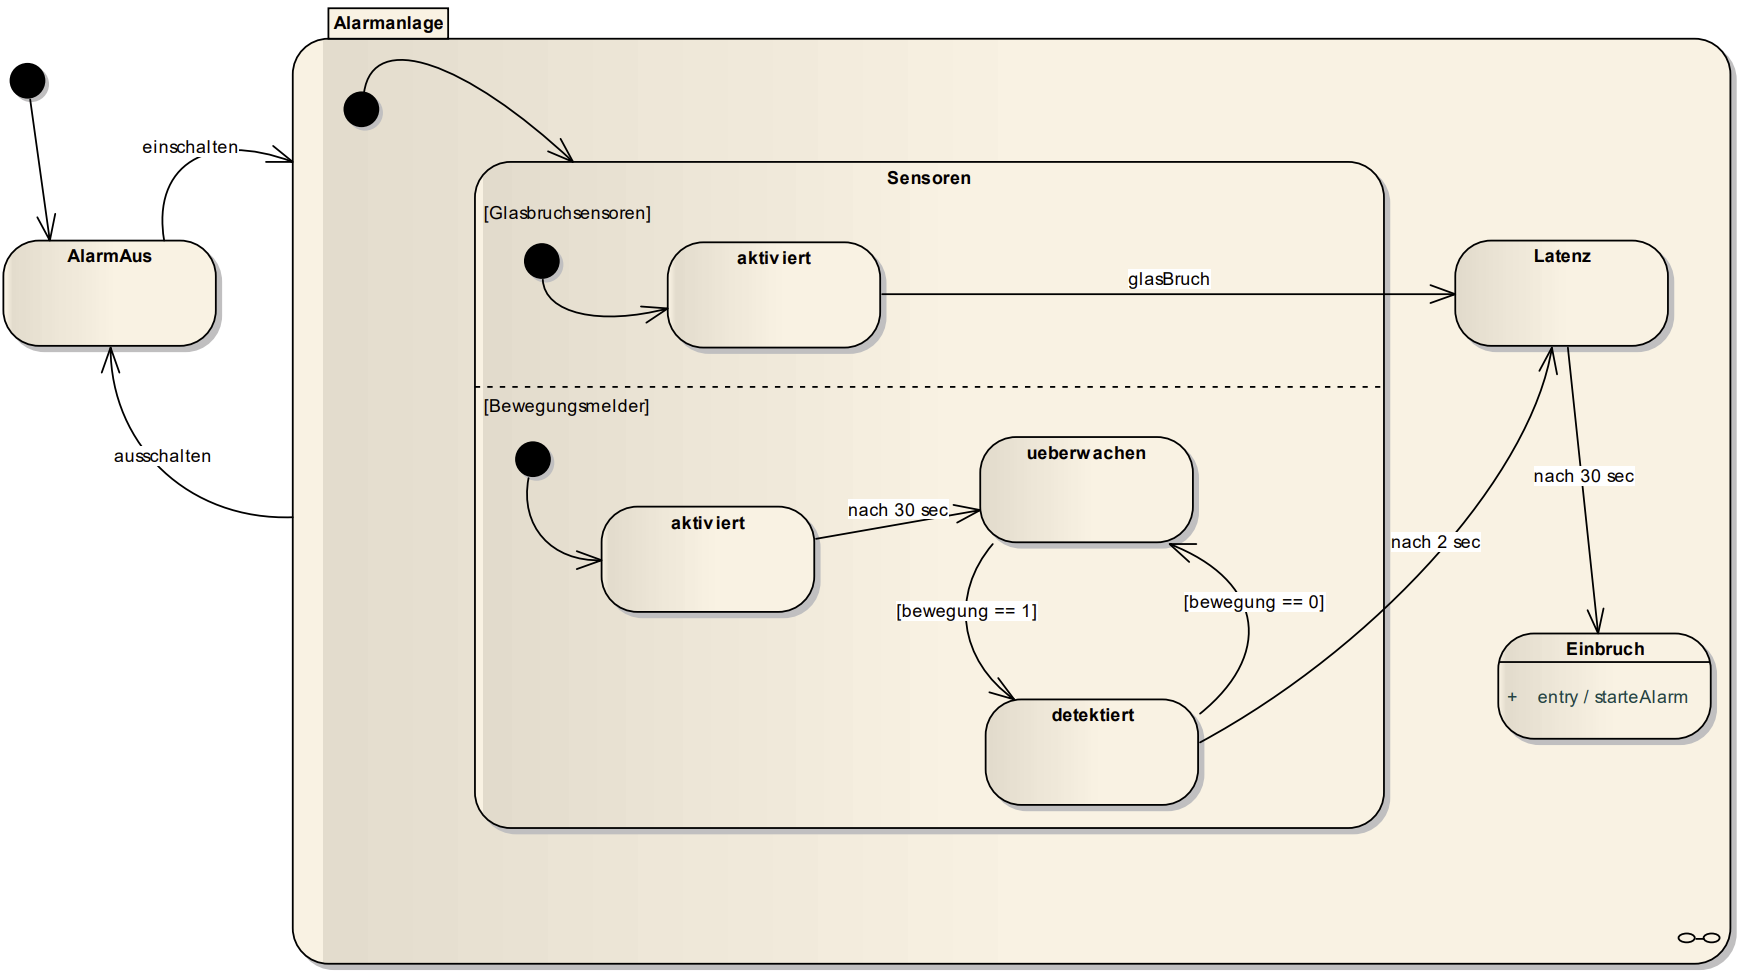
\includegraphics[width=\linewidth]{images/FSM/Bsp_Alarmanlage.png}
\end{itemize}
\newpage

% \section{Finite State Machine Realisierung}

\subsection{Realisierung von Flachen FSMs}
\begin{multicols}{2}
      \begin{itemize}
            \item Steuerkonstrukt (typischerweise mit switch-case)
                  \begin{itemize}
                        \item prozedural oder objektorientiert
                  \end{itemize}
            \item Definition und Abarbeitung einer Tabelle
                  \begin{itemize}
                        \item prozedural oder objektorientiert
                  \end{itemize}
            \item State Pattern (Gang of Four, GoF)
                  \begin{itemize}
                        \item nur objektorientiert
                  \end{itemize}
            \item Generisch mit Templates
                  \begin{itemize}
                        \item nur mit einer Sprache, die Templates unterstützt (z.B. C++)
                  \end{itemize}
            \item Alle Varianten haben wie immer sowohl Vor- als auch Nachteile
            \item Bei allen Varianten sind auch Variationen vorhanden
      \end{itemize}
\end{multicols}

\subsection{Realisierung mit Steuerkonstrukt (prozedural in C)}
\begin{figure}[H]
      \centering
      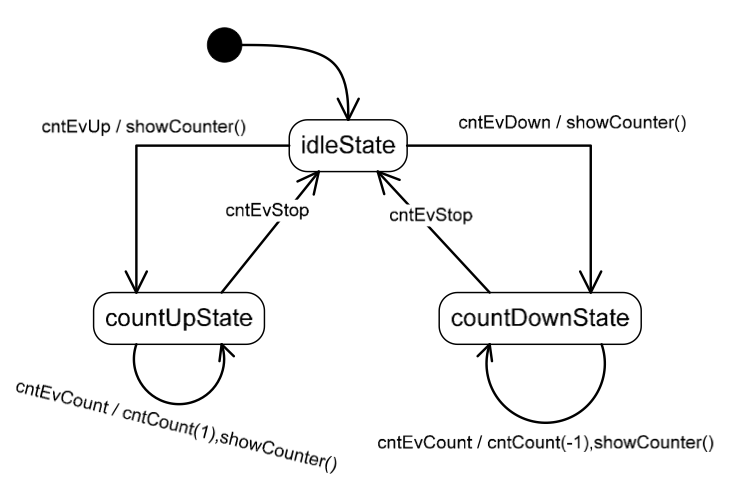
\includegraphics[scale = 0.35]{images/FSM/Up_down_counter}
\end{figure}
\begin{itemize}
      \item Zustände (States) werden in einem eunum definiert (nicht public!)
            \lstinputlisting[style=C, firstline=13, lastline=16]{snippets/Ctrl_C/counterCtrl.c}

      \item Ereignisse (Events) werden in einem enum definiert (public!)
            \lstinputlisting[style=C, firstline=12, lastline=16]{snippets/Ctrl_C/counterCtrl.h}

      \item Die FSM wird in zwei Funktionen implementiert
            \lstinputlisting[style=C, firstline=18, lastline=23]{snippets/Ctrl_C/counterCtrl.h}

      \item Der aktuelle Zustand der FSM wird in einer statischen Variablen gehalten
            \lstinputlisting[style=C, firstline=18, lastline=18]{snippets/Ctrl_C/counterCtrl.c}

\end{itemize}

\subsubsection{Vollständiger Code für prozedurales Steuerkonstrukt}
\lstinputlisting[style=C]{snippets/Ctrl_C/counterCtrl.h}
\lstinputlisting[style=C]{snippets/Ctrl_C/counterCtrl.c}
\lstinputlisting[style=C]{snippets/Ctrl_C/counter.h}
\lstinputlisting[style=C]{snippets/Ctrl_C/counter.c}
\lstinputlisting[style=C]{snippets/Ctrl_C/counterTest.c}

\subsubsection{Eigenschafteen der C-Version}
\begin{itemize}
      \item Von der FSM kann so wie sie implementiert ist nur eine Instanz vorkommen, dies kommt daher, dass der State static ist. Mögliche Lösung, State übergeben.
      \item Die Attribute der FSM (currentState) können nicht schön gekapselt werden
      \item Die Struktur ist recht einfach und kann gut erweitert werden
      \item Die Funktion cnt\_ctrlProcess() kann beliebig aufgerufen werden (z.B. aus einem periodischen Task, laufend, etc.)
      \item Die Struktur der FSM ist von aussen nicht sichtbar, der FSM werden nur die eingetretenen Events übertragen
      \item Bei exportierten Funktionen und Definitionen muss in C ein Modulkürzel vorangestellt werden (hier: cnt)
\end{itemize}


\subsection{Realisierung mit Steuerkonstrukt (Objektorientiert in
      C++)}

\begin{figure}[H]
      \centering
      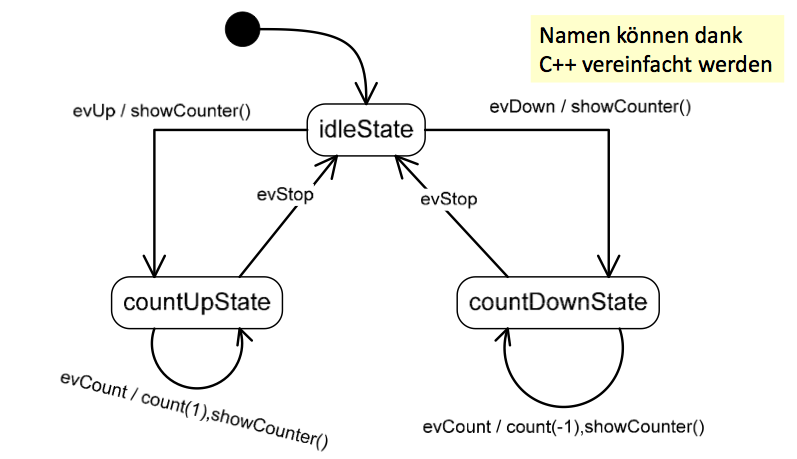
\includegraphics[scale = 0.35]{images/FSM/Up_down_counter_obj}
\end{figure}

\begin{itemize}
      \item Logisch gesehen funktioniert die objektorientierte Variante völlig identisch wie die prozedurale
      \item Dank des Klassenkonstrukts kann die FSM sauber gekapselt werden
      \item Der aktuelle Zustand der FSM (currentState) wird in einem Attribut der Klasse gehalten
            \begin{figure}[H]
                  \centering
                  \includegraphics[scale = 0.35]{images/FSM/klasseCounter}
            \end{figure}
      \item Mehrere Instanzen derselben FSM können einfach erstellt werden
      \item Ein Modulkürzel ist nicht notwendig, da alle Namen im Kontext von Klassen definiert werden
      \item Der Code wird eleganter, eine Performanceeinbusse ist nicht vorhanden
      \item States werden im \textbf{private-Teil} der Klasse mit einem enum definiert
            \lstinputlisting[style=Cpp, firstline=26, lastline=28]{snippets/Ctrl_Cpp/counterCtrl.h}
      \item Events werden im \textbf{public-Teil} der klasse mit einem enum definiert (public, weil die Events zur Schnittstelle gehören)
            \lstinputlisting[style=Cpp, firstline=16, lastline=19]{snippets/Ctrl_Cpp/counterCtrl.h}
      \item Die FSM wird in zwei Funktionen implementiert
            \lstinputlisting[style=Cpp, firstline=20, lastline=23]{snippets/Ctrl_Cpp/counterCtrl.h}
      \item \textbf{Entry-Actions} müssen überall dort hinzugefügt werden, wo in einen neuen Zustand gewechselt wird. Üblicherweise muss die Entry-Action für einen bestimmten Zustand bei mehreren Transitionen codiert werden.
      \item \textbf{Exit-Actions} müssen überall dort hinzugefügt werden, wo ein Zustand verlassen, d.h. in einen anderen Zustand gewechselt wird. Üblicherweise muss die Exit-Action für einen bestimmten Zustand bei mehreren Transitionen codiert werden.
\end{itemize}

\subsubsection{Vollständiger Code für objektorientiertes Steuerkonstrukt}
\lstinputlisting[style=Cpp]{snippets/Ctrl_Cpp/CounterCtrl.h}
\lstinputlisting[style=Cpp]{snippets/Ctrl_Cpp/CounterCtrl.cpp}

\subsection{Realisierung mit Tabelle}
\begin{itemize}
      \item Die Tabelle kann sowohl prozedural als auch objektorientiert implementiert werden.
      \item Die objektorientierte Variante verwendet einzig die Datenkapselung. Vererbung und Polymorphismus werden nicht benötigt
      \item Die objektorientierte Variante kann klarer und schöner strukturiert implementiert werden. Im folgenden wird nur diese Variante gezeigt, die C-Version kann jedoch einfach davon abgeleitet werden
      \item Die ganze FSM ist in einer Tabelle gespeichert
      \item Die Aktionen sind als Funktionen implementiert, in der Tabelle steht der entsprechende Funktionspointer
      \item Die Abarbeitung der FSM erfolgt mit Hilfe einer \textit{Execution Engine}, die in der Tabelle "nachschaut", was zu tun ist
      \item Die Execution Engine ändert sich nicht, wenn die FSM geändert wird
      \item Das Testprogramm ist völlig unverändert
      \item Die Schnittstelle von CounterCtrl (public-Teil) ist ebenfalls identisch
      \item Die Klasse Counter ändert auch nicht
      \item Die \textbf{einzige Änderung} liegt im private-Teil der
            CounterCtrl-Klasse und natürlich in deren Implementation
      \item Alle (Tansitions-)Aktionen werden als Methoden deklariert,
            \textit{Action} wird als Funktionspointer definiert. Diese Methoden müssen
            alle mit dem Funktionspointer übereinstimmen
            \lstinputlisting[style=Cpp, firstline=33, lastline=40]{snippets/Table_Simple/CounterCtrl.h}

      \item Die Transition wird als klasseninterne Struktur deklariert. Sie besteht
            aus
            \begin{itemize}
                  \item Aktueller Zustand
                  \item Event
                  \item Funktionspointer auf Aktionsmethode
                  \item Nächster Zustand
            \end{itemize}
            fsm[] wird als statischer offener Array deklariert.
            \lstinputlisting[style=Cpp, firstline=42, lastline=49]{snippets/Table_Simple/CounterCtrl.h}

      \item Tabellendefinition in CounterCtrl.cpp (Jede Transition bildet eine Zeile)
            \begin{figure}[H]
                  \centering
                  \includegraphics[scale = 0.5]{images/FSM/tabelle}
            \end{figure}
            \lstinputlisting[style=Cpp, firstline=14, lastline=22]{snippets/Table_Simple/CounterCtrl.cpp}

      \item Aufbau einer Aktionsmethode
            \lstinputlisting[style=Cpp, firstline=65, lastline=70]{snippets/Table_Simple/CounterCtrl.cpp}

      \item Performancesteigerung mit inline-Funktionen
            \begin{itemize}
                  \item Die Action-Funktionen sind oft recht kurz, dennoch werden diese Funktionen immer über einen Funktionspointer aufgerufen
                  \item Eine naheliegende Lösung ist, alle Action-Funktionen inline zu definieren
                  \item \textbf{Leider nützt das nichts}, denn eine Funktion wird niemals inlined, wenn ein Pointer auf diese Funktion verwendet wird. Und genau das wird in der Tabelle gemacht.
            \end{itemize}

      \item Execution Engine
            \lstinputlisting[style=Cpp, firstline=30, lastline=41]{snippets/Table_Simple/CounterCtrl.cpp}

            \begin{itemize}
                  \item Vor dem Aufrufen der Aktionen über den Funktionspointer müsste streng genommen überprüft werden, ob es sich um einen gültigen Pointer handelt $\rightarrow$ aus Performancegründen wird darauf verzichtet
                  \item Voraussetzung dafür ist, dass in der Tabelle immer ein gültiger Pointer auf eine Memberfukntion vorhanden ist. Wenn nichts zu tun ist, soll ein Pointer auf eine leere Funktion eingesetzt werden (im Beispiel der Pointer \&counterCtrl::actionDoNothing)
                  \item Da sich die Tabelle und die Execution Engine in derselben Datei befinden, ist dieses Vorgehen unproblematisch, bzw. sogar die bevorzugte Variante
            \end{itemize}

      \item Erweiterungsmöglichkeit: Wenn der Zustandsübergang nicht nur durch einen Event, sondern eine komplexe Prüfung (Event und Guard) ausgelöst wird, dann könnte der Eventeintrag in der Tabelle durch einen weiteren Funktionspointer auf eine Checkfunktion ersetzt werden
            \lstinputlisting[style=Cpp, firstline=33, lastline=33]{snippets/Table/CounterCtrl.h}
            \lstinputlisting[style=Cpp, firstline=36, lastline=36]{snippets/Table/CounterCtrl.h}
            \lstinputlisting[style=Cpp, firstline=51, lastline=57]{snippets/Table/CounterCtrl.h}
\end{itemize}

\subsubsection{Vollständiger Code für Tabellen-Realisation}
\lstinputlisting[style=Cpp]{snippets/Table/CounterCtrl.h}
\lstinputlisting[style=Cpp]{snippets/Table/CounterCtrl.cpp}

\subsection{Realisierung mit State Pattern}
\begin{itemize}
      \item Das Prinzip besteht aus einer abstrakten State-Basisklasse. Pro Zustand
            muss eine eigene Klasse definiert werden, die von dieser abstrakten
            Basisklasse erbt.
      \item Die Realisierung nutzt das Polymorphismus-Konzept, jede konkrete
            State-Klasse ist ein \textit{Singleton}
      \item Statt lange switch-case-if-Konstrukte wird beim State Pattern ein
            bestimmter Zustand vollständig in einer eigenen Klasse realisiert. Die Logik
            wird somit aufgeteilt.
      \item \textbf{Context} definiert die interessierenden Schnittstellen für
            Clients, unterhält eine Instanz einer konkreten Unterklasse von State, die den
            aktuellen Zustand definiert, bzw. repräsentiert
      \item \textbf{State} definiert eine schnittstelle zur FMS in Form einer
            abstrakten Klasse
      \item \textbf{ConcreteStateX Unterklassen} jede Unterklasse implementiert
            genau einen Zustand (ist Singleton)
            \begin{figure}[H]
                  \centering
                  \includegraphics[scale = 0.3]{images/FSM/state_pattern}
            \end{figure}
      \item Das State Pattern definiert die Zuständigkeit der state Transition nicht
      \item Die Transitionen könnten in der Context-Klasse definiert werden. Der
            Nachteil dieser Variante ist, dass dort zentral sehr viel Intelligenz vorhanden
            sein müsste. Da diese Klasse auch den Zugriff zur Aussenwelt darstellt, sollte
            sie möglichst schlank sein.
      \item Die bessere Variante ist, wenn die State-Klassen auch gleich ihre
            Transitionen realisieren. Diese Variante wird oft mittels friend-Deklaration
            realisiert, was jedoch nicht nötig ist
      \item Schnittstelle zur State Machine; CounterCtrl ist die Context-Klasse; process() entspricht request()
\end{itemize}

\begin{center}
      \includegraphics[width=0.7\linewidth]{./images/FSM/klassendiagramm}
\end{center}

\begin{itemize}
      \item counterCtrl.h : Schnittstelle zur FSM
            \lstinputlisting[style=Cpp]{snippets/Pattern_Action/CounterCtrl.h}

      \item counterCtrl.cpp
            \lstinputlisting[style=Cpp]{snippets/Pattern_Action/CounterCtrl.cpp}

      \item class CounterState: Interface
            \lstinputlisting[style=Cpp]{snippets/Pattern_Action/CounterState.h}
            \begin{itemize}
                  \item CounterState::changeState(...)
                        \begin{itemize}
                              \item Diese Funktion könnte für diese Anwendung auch wegoptimiert werden, aus Kompatibilitätsgründen für (noch folgende) Erweiterungen soll sie jedoch beibehalten werden
                        \end{itemize}
                  \item CountUpState::getInstance() ist eine statische Funktion mit class scope. Sie ist zusammen mit instance charakteristisch für das Singleton
                  \item CountUpState::handle() ist spezifisch für diesen State zu implementieren
                  \item CountUpState::CountUpState ist der private Default Ctor der verhindert, dass von dieser Klasse Objekte erzeugt werden können
                  \item CountUpState::entryAction() und CountUpState::exitAction() müssen nur dann deklariert und überschrieben werden, wenn es wirklich etwas Spezifisches zu tun gibt, andernfalls wird die Default-Implementation der Basisklasse genommen
            \end{itemize}
      \item class CounterState: Implementation
            \lstinputlisting[style=Cpp]{snippets/Pattern_Action/CounterState.cpp}
\end{itemize}

\subsection{Realisierung von hierarchischen State Machines}
\begin{itemize}
      \item Toolunterstützung
            \begin{itemize}
                  \item IBM Rhapsody, MathWorks Matlab/Simulink mit RT Workbench, u.a.
            \end{itemize}
      \item QP-Framwork
            \begin{itemize}
                  \item Framwork für Ausführung mit oder ohne Betriebssystem
                  \item Ressourcenbedarf: 1kB RAM, 10kB ROM
                  \item Targets: Cortex-M4
                  \item QP-nano für kleine Controller (z.B. MSP430, 8051, PIC, AVR)
                  \item Ressourcenbedarf QP-nano: 100 Bytes RAM, 2kB ROM
            \end{itemize}
\end{itemize}

\newpage

% \section{Modularisierung}
Modularisierung ist die Aufteilung eines Ganzen in Teile, die als Module oder Komponenten bezeichnet werden. Bei geeigneter Form und Funktion können sie zusammengefügt werden oder über entsprechende Schnittstellen interagieren.

\subsection{Grundprinzip}
\begin{itemize}
  \item Divide et impera (Teile und herrsche)
  \begin{itemize}
    \item Problem aufteilen und Unterprobleme einzeln angehen
    \item Zuerst Grobentwurf, dann verfeinern (Top-Down-Prinzip)
  \end{itemize}
  \item \textbf{Ziel:} Reduktion der Komplexität
\end{itemize}

\subsection{Motivation}
Bei Kleinstsoftware braucht es kein systematisches Design, da man diese meist auch nicht ausbauen möchte. Vernünftige Softwaresysteme benötigen einen systematischen Designansatz mit einem strukturierten Aufbau.\\\\
Wichtig ist daher:
\begin{itemize}
	\item Entwicklung im Team vs. One-person-show
	\item Schnittstellen definieren
\end{itemize}

\subsection{Information Hiding}
\begin{itemize}
  \item Nutzer des Moduls braucht nur die Schnittstelle zu kennen (*.h files)
  \item Über inneren Aufbau dürfen keine Annahmen getroffen werden
  \item Der innere Aufbau (*.cpp files) muss nicht bekannt sein
\end{itemize}

\subsection{Hauptkriterien der Zerlegung}
\begin{itemize}
  \item Kopplung/Coupling
  \begin{itemize}
    \item Mass für Komplexität der Schnittstelle
  \end{itemize}
  \item Kohäsion/Cohesion
  \begin{itemize}
    \item Aussage wie stark eine funktionale Einheit wirklich zusammengehört
    \item Mass für die Stärke des inneren Zusammenhangs
  \end{itemize}
\end{itemize}

\textbf{Ziel:} Schwache Kopplung, starke Kohäsion

\begin{multicols}{2}
\includegraphics[width=\linewidth]{images/Modularisierung/BeispieleKopplungKohaesion.png}
\vfill\null
\begin{itemize}
	\item Bild a: Schwache Kopplung, starke Kohäsion (gut)
	\item Bild b: Starke Kopplung, schwache Kohäsion (schlecht)
\end{itemize}
\vfill\null
\end{multicols}

\begin{multicols}{2}
\subsection{Definitionen Kopplung}
\begin{itemize}
  \item Keine direkte Kopplung (Schwache Kopplung $\rightarrow$ \textbf{GUT})
  \item Datenkopplung
  \begin{itemize}
    \item Kommunikation ausschliesslich über Parameter
  \end{itemize}
  \item Datenbereichskopplung
   \begin{itemize}
    \item Modul hat Zugriff auf Datenstruktur eines anderen Moduls
    \item Es werden nur einzelne Komponenten benötigt
  \end{itemize}
  \item Steuerflusskopplung (Control Flow)
  \begin{itemize}
    \item Modul beeinflusst Steuerfluss eines anderen Moduls
  \end{itemize}
  \item Globale Kopplung
  \begin{itemize}
    \item Kommunikation über globale Variabeln
    \item Jedes Modul hat Zugriff
  \end{itemize}
  \item Inhaltskopplung (Starke Kopplung $\rightarrow$ \textbf{SCHLECHT})
  \begin{itemize}
    \item Aus einem Modul werden lokale Daten eines anderen Moduls modifiziert,
    obwohl dieses Modul NICHT vom anderen Modul aufgerufen wird.
    \item \textbf{Todsünde}
  \end{itemize}
\end{itemize}
\columnbreak
\subsection{Definitionen Kohäsion}
\begin{itemize}
  \item Funktionale Kohäsion (Starke Kohäsion $\rightarrow$ \textbf{GUT})
  \begin{itemize}
    \item Teile einer Einheit bilden zusammen eine Funktion
  \end{itemize}
  \item Sequentielle Kohäsion
   \begin{itemize}
    \item Teilfunktionen einer Einheit werden nacheinander ausgeführt
    \item Das Ergebnis einer Teilfunktion ist die Eingabe der nächsten
  \end{itemize}
  \item Kommunikative Kohäsion
  \begin{itemize}
    \item Teilfunktionen einer Einheit werden auf den gleichen Daten ausgeführt
    \item Reihenfolge spielt keine Rolle
  \end{itemize}
  \item Prozedurale Kohäsion
  \begin{itemize}
    \item Teilfunktionen werden nacheinander ausgeführt
    \item Sind über Steuerfluss verknüpft
  \end{itemize}
  \item Zeitliche Kohäsion
  \begin{itemize}
    \item Teile einer Einheit sind alle zu einer bestimmten Zeit auszuführen
  \end{itemize}
  \item Logische Kohäsion
  \begin{itemize}
    \item Teilfunktionen einer Einheit gehören zu einer Klasse
  \end{itemize}
  \item Zufällige Kohäsion (Schwache Kohäsion $\rightarrow$ \textbf{SCHLECHT})
  \begin{itemize}
    \item Teilfunktionen einer Einheit haben keinen sinnvollen Zusammenhang
  \end{itemize}
\end{itemize}
\end{multicols}
\begin{minipage}{9cm}
\subsubsection{Ziele bezüglich Kohäsion}
  \begin{itemize}
  \item Kohäsion maximieren
  \item Idealerweise führt eine Unit nur eine Aufgabe (Funktion) aus
  \item Starke Kohäsion steigert
    \begin{itemize}
    \item Wartbarkeit
    \item Änderbarkeit
    \item Verständlichkeit
    \end{itemize}
  \item \textbf{Zusammengehörendes zusammen nehmen!}
  \item \textbf{Starke Kohäsion führt zu schwacher Kopplung, aber nicht umgekehrt!!}
  \end{itemize}
\end{minipage}
\hfill
\begin{minipage}{9cm}
  \subsubsection{Bestimmung der Kohäsion}
  \includegraphics[width=9cm]{images/Modularisierung/Kohaesionsbestimmung.png}
\end{minipage}

\subsection{Schlechte vs. gute Modularisierung}
\begin{minipage}[t]{10cm}
\textbf{Beispiel schlechter Modularisierung:}\\
\includegraphics[width=9cm]{images/Modularisierung/SchlechtesBeispielModularisierung.png}
\end{minipage}
\begin{minipage}[t]{8cm}
\textbf{Beispiel guter Modularisierung:}\\
\includegraphics[width=8cm]{images/Modularisierung/GutesBeispielModularisierung.png}
\end{minipage}

\subsection{In bestehendem Projekt zurechtfinden}
\begin{itemize}
	\item Die Schnittstelle muss in den Headerfiles beschrieben werden
	\item Dort muss man alles finden, was wichtig ist, d.h. es müssen zuerst die Headerfiles studiert werden
	\item Wenn man das Projekt nur nutzen soll, dann sollte man im Normalfall keinen Grund finden, auch die Definitionsfiles (*.c, *.cpp) anschauen zu müssen
\end{itemize}

\subsection{Package-Diagramm}
\begin{itemize}
	\item ist bekannt aus OOAD
	\item Ein Package besteht aus mindestens einer, üblicherweise aus mehreren Klassen, die zusammengehören (Stichwort: Kohäsion)
	\item Im Package-Diagramm kann dargestellt werden, welche Packages mit welchen anderen Packages Verbindungen haben (dürfen), d.h. die Abhängigkeiten zwischen Packages können sichtbar gemacht werden
	\item In C++ wird das Packagekonzept mit Namespaces umgesetzt, d.h. ein Namespace entspricht einem Package
\end{itemize}

% %!TEX root = ../EmbSW1.tex
\section{Event Based Systems}
\subsection{Reaktive Systeme}
Ein Reaktives System befindet sich in ständiger Interaktion mit der Umgebung, wobei die Umgebung dominiert und das System sich dieser unterordnet.
\begin{itemize}
	\item Viele Embedded Systems sind auch reaktive Systeme
	\item Reaktive Systeme reagieren auf (oft externe) Ereignisse
	      \begin{itemize}
		      \item Digitale Inputs
		      \item Erreichen von analogen Schwellwerten
		      \item Timer
		      \item Buttonclicks und ähnliches in GUI
		      \item etc.
	      \end{itemize}
	\item Häufig bestehen auch Echtzeitanforerungen an reaktive Systeme
\end{itemize}

\subsection{Umsetzung von Ereignissen}
\begin{itemize}
	\item Ereignisse sind per Definition asynchron
	\item Ein "'normales"' Programm ist immer synchron (das Programm gibt vor, was wann ausgeführt wird)
	\item Ereignisse können von synchronen Programmen durch Polling verarbeitet werden (synchron)
	      \begin{itemize}
		      \item[+] einfach zu implementieren
		      \item sehr viele Leerabfragen $\rightarrow$ unnötige Prozessorbelastung
		      \item[$\bullet$] Leerabfragen können durch periodische Abfragen (Kopplung an Timer) reduziert aber nicht vermieden werden.
		      \item[$\bullet$] Die maximale Reaktionszeit wird durch die Abfrageperiode und die Anzahl Abfragen definiert
	      \end{itemize}
	\item Interrupt (asynchron)
	      \begin{itemize}
		      \item Non-vectored Interrupt (zentral)
		            \begin{itemize}
			            \item Alle Interrupts verzweigen zu einer gemeinsamen Adresse. Dort wird die Ursache bestimmt und zu einer spezifischen Behandlungsroutine verzweigt.
		            \end{itemize}
		      \item Vectored Interrupt (spezifisch)
		            \begin{itemize}
			            \item In einer Tabelle (Interruptvektortabelle) wird gespeichert, wohin bei welchem Interruptvektor verzweigt werden muss.
		            \end{itemize}
	      \end{itemize}
	\item	Interruptvektortabelle (IVT)
	      \begin{itemize}
		      \item Für jeden Vektor muss eingetragen werden, welches die Anfangsadresse der Interrupt Service Routine (ISR) ist, d.h. die IVT ist nichts anderes als eine Tabelle (Array) von Funktionspointern.
	      \end{itemize}
\end{itemize}

\subsection{Model View Controller (MVC) aka Observer Pattern}
\begin{multicols}{2}
	\begin{itemize}
		\item Beim MVC wirkt das Model als Server, die Views sind Clients
		\item Jeder Client meldet beim Server an, welche Ereignisse ihn interessieren
		\item Diese Anmeldung, bzw. Registrierung erfolgt über eine Funktion, welche der Server anbietet:
		      \begin{lstlisting}[style=C]
int foo_registerCb(foo_Event e, foo_cbFunction f);
// registers function 'f' on event 'e'
// sometimes called attach()
		\end{lstlisting}
		\item Der Server trägt diesen Funktionspointer f in eine Tabelle ein und ruft bei Eintreten des Ereignisses alle registrierten Funktionen der Reihe nach je über den eingetragenen Funktionspointer auf
	\end{itemize}
	\columnbreak
	\includegraphics[width=\linewidth]{images/EventBasedSystems/MVC}
\end{multicols}

\subsubsection{Umsetzung der Callback-Funktionen in C}
\begin{itemize}
	\item Funktionspointer \lstinline[style=C]{foo_cbFunction} zu Callback-Funktionen definieren\\
	      Annahme: Callback-Funktionen haben die Schnittstelle \lstinline[style=C]{void f(int);}
	      \begin{lstlisting}[style=C]
typedef void (*foo_cbFunction)(int);
	\end{lstlisting}

	\item Tabelle von Funktionspointern für jeden Event definieren
	      \begin{lstlisting}[style=C]
foo_cbFunction evClient[evNum] = {0};
	\end{lstlisting}

	\item Aufruf der registrierten Clientfunktionen beim Eintreten des Events
	      \begin{lstlisting}[style=C]
for (i = 0; i < evNum; ++i)
{
  if (evClient[i] != 0) // entry found
  {
    evClient[i](arg);   // call client through function ptr
  }
}
	\end{lstlisting}
\end{itemize}

\subsubsection{Vorteile der Callback-Funktionen}
\begin{itemize}
	\item Die Views werden asynchron genau informiert, wenn sich etwas geändert hat im Model
	\item An und für sich sind alle registrierten Funktionen nichts anderes als Eventhandler eines bestimmten Events
	\item Dadurch wird die Darstellung (die Definition der registrierten Funktionen) sauber von den Daten (Model) entkoppelt
\end{itemize}

\subsubsection{Observer Pattern}
\includegraphics[height=6cm]{images/EventBasedSystems/ObserverPattern.png}
% \section{Computerarithmetik}

\subsection{Ganzzahlig}
\begin{tabular}{|p{3cm}|p{4.5cm}|p{4.5cm}|p{4.5cm}|}
	\hline
	Darstellung & Sign Magnitude & 1er Komplement & 2er Komplement\\
	\hline
	Zahlenbereich & $-(2^{n-1}-1)$ bis $+(2^{n-1}-1)$ & $-(2^{n-1}-1)$ bis +$(2^{n-1}-1)$ & $-2^{n-1}$ bis +$(2^{n-1}-1)$\\
	\hline
	Vorteil & Vorzeichen kann einfach durch Vorzeichenbit festgestellt werden. & Vorzeichen kann einfach durch MSB festgestellt werden. Addition und Subtraktion einfach realisierbar. & Vorzeichen kann einfach durch MSB festgestellt werden. Addition und Subtraktion einfach realisierbar \\
	\hline
	Nachteil & Positive und negative Null. Addition/Subtraktion kompliziert. & Positive und negative Null. & Bereich nicht ganz symmetrisch\\
	\hline
	Beispiel +5 & 0101 & 0101 & 0101 \\
	Beispiel -5 & 1101 & 1010 & 1011 \\
	\hline
\end{tabular}

\subsubsection{Addition/Subtraktion}
Wird direkt mit der Arithmetic Logic Unit (ALU) durchgeführt.

\subsubsection{Multiplikation}
\paragraph {Multiplikation mit Zweierpotenzen}
Die Multiplikation mit Zweierpotenzen ist ein Spezialfall, der sehr effizient umgesetzt werden kann. Die Multiplikation einer Zahl $x$ mit $2^n$ entspricht einem Schieben der Zahl $x$ um $n$ Stellen nach links.

\paragraph{Allgemeine Multiplikation}
\begin{multicols}{2}
	Implementation algorithmisch: Langsam, wenig Aufwand
	\begin{itemize}
		\item Mikroprogramm
		\item Softwareemulation
	\end{itemize}
	Implementation Hardware: Schnell, viel Aufwand
	\begin{itemize}
		\item In vielen uC's drin, vor allem RISC (MSP430)
		\item Im DSP ist HW-Multiplizierer ein Muss (wichtige Multiply-Accumulate-Funktion (MAC))
	\end{itemize}
	\columnbreak
	\includegraphics[width=0.3\textwidth]{images/Arithmetik/Ganzzahlig_Multiplikation}
\end{multicols}

\subsubsection{Division}
\paragraph {Division mit Zweierpotenzen}
Die Division durch Zweierpotenzen ist ein Spezialfall, der sehr effizient umgesetzt werden kann. Die Division einer Zahl $x$ durch $2^n$ entspricht einem Schieben der Zahl $x$ um $n$ Stellen nach rechts.

\paragraph {Allgemeine Division}
Implementation algorithmisch: Langsam, wenig Aufwand
\begin{itemize}
	\item Mikroprogramm
	\item Softwareemulation
\end{itemize}
Implementation Hardware: Schnell, viel Aufwand
\begin{itemize}
	\item da die Division die seltenste Operation ist, wird speziell bei Microcontrollern nur selten ein Hardware-Dividierer verwendet
\end{itemize}

\subsubsection{Skalierung}
\begin{itemize}
	\item Aus Effizienzgründen wird insbesondere bei Mikrocontrollern versucht, so viel wie möglich mit Integer-Arithmetik zu lösen
	\item Quantisierung auf 1 Bit kann bei kleinen Werten zu Ungenauigkeiten führen
	\item Lösung: durch Skalierung soll Dynamikbereich, d.h. der Wertebereich der ganzen Zahl, möglichst ausgenutzt werden
	\item Skalierungen mit Zweierpotenzen sind viel effizienter als solche mit Dezimalzahlen
	\item \textbf{Wenn möglich immer mit Zweierpotenzen skalieren}
\end{itemize}

\subsection{Arithmetische Schaltungen}
\subsubsection{Addierer}
Wichtigste arithmetische Funktion, n-Addierer werden auf 1-Bit Addierer zurück geführt.
\paragraph{1 Bit Halbaddierer:}
\begin{minipage}{0.5\textwidth}
	\centering
	\begin{tabular}{|c | c | c | c |}
		\hline
		A & B & Sum & Carry\\
		\hline
		0 & 0 & 0 & 0\\
		\hline
		0 & 1 & 1 & 0\\
		\hline
		1 & 0 & 1 & 0\\
		\hline
		1 & 1 & 0 & 1\\
		\hline
	\end{tabular}
\end{minipage}
\begin{minipage}{0.9\textwidth}
	\centering
	\begin{flushleft}
		{\includegraphics[width=0.3\textwidth]{images/Arithmetik/halbaddierer.png}}
	\end{flushleft}
\end{minipage}\\ \\

\paragraph{1 Bit Volladierer:}
\begin{minipage}{0.35\textwidth}
	\begin{tabular}{|c | c | c | c | c |}
		\hline
		A & B & Carry In & Sum & Carry Out\\
		\hline
		0 & 0 & 0 & 0 & 0\\
		\hline
		0 & 0 & 1 & 1 & 0\\
		\hline
		0 & 1 & 0 & 1 & 0\\
		\hline
		0 & 1 & 1 & 0 & 1\\
		\hline
		1 & 0 & 0 & 1 & 0\\
		\hline
		1 & 0 & 1 & 0 & 1\\
		\hline
		1 & 1 & 0 & 0 & 1\\
		\hline
		1 & 1 & 1 & 1 & 1\\
		\hline
	\end{tabular}
\end{minipage}
\begin{minipage}{0.9\textwidth}
	\begin{flushleft}
		{\includegraphics[width=0.7\textwidth]{images/Arithmetik/volladdierer.png}}
	\end{flushleft}
\end{minipage}

\paragraph {Ripple Carry Adder (4 Bit)}
\includegraphics[width=1\textwidth]{images/Arithmetik/Ripple_Carry_Adder}
Das niederwertige Carry-Bit wird immer an die nächst höhere Position weitergereicht. Dadurch dauert es eine gewisse Zeit, bis das MSB korrekt ist. Für hohe Wortbreiten zu langsam.

\paragraph{Carry Select Adder}
\begin{itemize}
	\item Obere Worthälfte wird zweimal berechnet
	\begin{itemize}
		\item einmal für Carry-In = 0
		\item einmal für Carry-In = 1
	\end{itemize}
	\item Die untere Worthälfte und die beiden oberen Worthälften werden gleichzeitig berechnet.
	\item Das richtige Resultat der oberen Worthälfte wird ausgewählt sobald das Carry der unteren Worthälfte feststeht.
	\item Bei einem $n$ Bit breiten Adder wird idealerweise in $\sqrt{n}$ breite Blöcke aufgeteilt
	\item Die Ausführungszeit steigt dann nicht linear, sondern nur mit $\sqrt{n}$
	\item Kosten: Erhöhter Hardwareaufwand
\end{itemize}

\paragraph{Carry Look-Ahead Adder}
	\begin{multicols}{2}
		\begin{itemize}
		\item Carrymuss bei jeder Bitposition $i$ entweder fortgepflanzt (propagate, $p_i$) oder generiert (generate, $g_i$) werden.
		\item  $p_i$ und $g_i$ sind nur von den Eingängen $a_i$ und $b_i$ abhängig, nicht aber von den Carries der vorherigen Stufen.
		\begin{equation}
			p_i = a_i \oplus b_i \newline
		\end{equation}
		\begin{equation}
		g_i = a_i * b_i
		\end{equation}
		\begin{equation}
		c_{i+1} = g_i + p_i * c_i
		\end{equation}
		\item  Jedes einzelne Carry kann somit als zweistufige Logik von verschiedenen $p_i$ und $g_i$ implementiert werden.
	\end{itemize}
\columnbreak
	\includegraphics[width=0.5\textwidth]{images/Arithmetik/Carry_Look_Ahead_Adder}
\end{multicols}

\subsubsection{Subtrahierer}
\begin{equation}
A-B = A + (-B)
\end{equation}
\begin{itemize}
	\item Subtraktion wird zurückgeführt auf Addition
	\item (-B) kann gebildet werden, indem alle Bits von B invertiert werden und 1 addiert wird.
	\item 1 addieren erfolgt durch Anlegen einer '1' bei $Carry_0$
	\item Damit der Addierer mit minimalem Zusatzaufwand auch als Subtrahierer verwendet werden kann, wird deshalb auch an der Bitposition 0 ein Volladdierer eingesetzt
\end{itemize}

\subsubsection{Schiebeeinheit (Shifter)}
\begin{itemize}
	\item Ein Shifter kann mit einem Schieberegister implementiert werden
	\item Der Nachteil dabei ist, dass pro Clockzyklus nur um ein Bit nach links oder rechts geschoben werden kann. Zudem ist das Schieberegister eine sequentielle Schaltung und benötigt Flip Flops.
	\item Oft muss um eine beliebige Anzahl Stellen möglichst  in einem Schritt geschoben werden
	\item Schieben kann auch mittels einer kombinatorischen Schaltung erreicht werden
	\item In der Praxis wird meist ein \textbf{Barrel Shifter} eingesetzt. Dieser kann innerhalb eines Zyklus um eine beliebige Anzahl Stellen schieben. Der Barrel Shifter ist rein kombinatorisch.
\end{itemize}

\begin{multicols}{2}
	\paragraph{Kombinatorischer 8 Bit Shifter nach links (C=0) bzw. rechts (C=1)}
	\includegraphics[width=0.3\textwidth]{images/Arithmetik/Shifter_1}

	\paragraph{4 Bit Crossbar Barrel Shifter}
	\includegraphics[width=0.2\textwidth]{images/Arithmetik/Shifter_2}
\end{multicols}

\subsubsection{Sättigungsarithmetik}
\begin{itemize}
	\item Besonders bei DSPs wird die Sättigungsarithmetik als Option eingesetzt
	\item Wenn der maximal darstellbare Wert inkrementiert werden soll, ergibt das nicht einen Overflow sondern der Wert bleibt auf seinem Maximalwert
	\item Analog wird der minimale Wert behandelt: bei signed Typen verbleibt der minimale negative Wert, bei unsigned Typen der Wert Null
\end{itemize}

\subsection{Fixpunkt (Fixed Point)}
\begin{itemize}
	\item Die Hardware für Fixed Point Arithmetic ist einfacher als die Floating Point Arithmetic, d.h. sie kann einfacher implementiert werden
	\item Wie der Name sagt, sitzt der Dezimalpunkt an einer fixen Stelle. Die Stellen rechts vom Dezimalpunkt werden als negative Zweierpotenzen interpretiert
	\item  Für Fixed Point-Berechnungen kann die Integereinheit verwendet werden
	\item Eigentlich erhält das LSB einfach nicht mehr den Wert 1, sondern beispielsweise den Wert $2^{-6}$, d.h $\frac{1}{64} = 0.015625$
	\item  Davon ausgehend kann mit der Integereinheit ganz normal gerechnet werden. Fixed Point Berechnungen sind deshalb sehr effizient
\end{itemize}

\subsection{Gleitkomma (Floating Point)}
\begin{multicols}{2}
	\begin{equation}
	(-1)^S\cdot M \cdot B^E
	\end{equation}
	S = Vorzeichen (float: 1 bit double: 1 bit)\\
	M = Mantisse (float: 23 bit double: 52 bit)\\
	B = Basis \\
	E = Exponent (float: 8 bit double: 11 bit)\\
\columnbreak
	\includegraphics[width=0.5\textwidth]{images/Arithmetik/floating_point}
\end{multicols}

\subsubsection{Floating Point Unit (FPU)}
\begin{itemize}
	\item Eine FPU ist eine Hardwareimplementation für die Berechnung von Floating Point Zahlen
	\item Eine FPU-Implementation rechnet die FP-Operationen mindestens eine Grössenordnung schneller als Softwareimplementationen
	\item Nebst den Grundrechenarten rechnet die FPU auch Wurzeln, teilweise auch trigonometrische Funktionen, etc.
\end{itemize}

\subsubsection{Addition}
\begin{enumerate}
	\item Die beiden Exponenten subtrahieren, um festzustellen, welcher der grössere ist. Der grössere Exponent wird als resultierender Exponent verwendet. Die Mantisse der kleineren Zahl muss zudem vor der Addition um diesen Differenzbetrag verschoben werden.
	\item Die Mantisse der kleineren Zahl verschieben und zur grösseren addieren.
	\item Die Mantisse wieder normalisieren, d.h. für die Mantisse M muss immer gelten: $1 \leq M \leq 2$. Dies bedingt unter Umständen auch eine Anpassung des Exponenten.
\end{enumerate}
Für einen Floating Point Adder werden mindestens folgende Elemente benötigt: Integer-Addierer/Subtrahierer, Komparatoren und Schiebeeinheiten (Shifter)

\subsubsection{Subtraktion}
Der Floating Point Subtrahierer kann analog zum Addierer implementiert werden.

\subsubsection{Multiplikation}
\begin{equation}
	m_1 \cdot B^{e1} \cdot m_2 \cdot B^{e2} = m_1 \cdot m_2 \cdot B^{e1 + e2}
\end{equation}
\begin{enumerate}
	\item Die beiden Exponenten müssen addiert werden
	\item Die beiden Mantissen müssen multipliziert werden
	\item Die Mantisse wieder normalisieren, d.h. für die Mantisse M muss immer gelten: $1 \leq M \leq 2$. Dies bedingt unter Umständen auch eine Anpassung des Exponenten.
\end{enumerate}
Für einen Floating Point Multiplier werden mindestens folgende Elemente benötigt: Integer-Addierer/Subtrahierer, Integer-Multiplizierer und Schiebeeinheiten (Shifter)

\subsubsection{Division}
\begin{equation}
\frac{m_1 \cdot B^{e1}}{m_2 \cdot B^{e2}} = \frac{m_1}{m_2} \cdot B^{e1 - e2}
\end{equation}
\begin{enumerate}
	\item Die beiden Exponenten müssen subtrahiert werden
	\item  Die beiden Mantissen müssen dividiert werden
	\item Die Mantisse wieder normalisieren, d.h. für die Mantisse M muss immer gelten: $1 \leq M \leq 2$. Dies bedingt unter Umständen auch eine Anpassung des Exponenten.
\end{enumerate}
Für einen Floating Point Divider werden mindestens folgende Elemente benötigt: Integer-Addierer/Subtrahierer, Integer-Dividierer und Schiebeeinheiten (Shifter) \\
Die Floating Point Division ist relativ selten (ca. 5\% der Grundrechenarten im Normalfall). Aus diesem Grund wird oft kein Hardware-Dividierer angeboten. Häufig wird eine Multiplikation mit der Reziproken gerechnet. Die Reziproke kann nur mit Additionen und Multiplikationen gerechnet werden
\begin{equation}
\frac{x}{y} = \frac{1}{y} \cdot x
\end{equation}

\subsubsection{Berechnung von beliebigen Kurvenverläufen}
\begin{itemize}
	\item Der Verlauf von beliebigen Kurven wird häufig in Lookup Tables gespeichert
	\item Für Werte zwischen zwei Stützwerten wird interpoliert, normalerweise linear
	\item Die Genauigkeit nimmt offensichtlich zu, je mehr und je genauere Stützwerte gespeichert werden
	\item Denkbar sind auch Approximationen, wobei nur mit Additionen, Subtraktionen und Multiplikationen gearbeitet werden darf
\end{itemize}

\subsubsection{Newton-Raphson}
Um eine unäre Funktion wie $sin(x)$ zu berechnen, kann man die Taylorreihe verwenden $sin(x) = x - \frac{x^3}{3!} + \frac{x^5}{5!} - \frac{x^7}{7!}\cdots$ Die Koeffizienten könnten gespeichert werden, jedoch ist die Konvergenz trotz dieser Vereinfachung langsam.
Eine Methode, welche schneller konvergiert ist das Newton-Raphson Verfahren:
\begin{equation}
y_{k+1} = y_k - \frac{f(y_k)}{\frac{\partial}{\partial y}f(y_k)}
\end{equation}
Zur Berechnung einer Reziproken $g(x)=\frac{1}{x}=y$ ergibt sich folgende Formel:
\begin{equation}
y_{k+1} = y_k\cdot (2-x\cdot y_k)
\end{equation}
Wobei $x$ die Zahl aus dem Reziprokwert ist und $y_k$ ein vernünftiger Anfangswert ist. \\

Somit kann auch die Quadratwurzel berechnet werden und zwar via: $\frac{1}{\sqrt{x}} \cdot x = \sqrt{x}$\\
Wobei der Bruch $\frac{1}{\sqrt{x}}$ wie folgt berechnet werden kann:
\begin{equation}
y_{k+1} = 0.5y_k\cdot (3-x\cdot y_k^2)
\end{equation}
Das Newton Verfahren konvergiert quadratisch, d.h mit jedem Durchlauf kann die Genauigkeit verdoppelt werden.

\begin{multicols}{2}
	\paragraph{Herleitung $\frac{1}{x}$}
	\begin{equation}
	g(x)=\frac{1}{x} \equiv y \rightarrow x=\frac{1}{y}
	\end{equation}
	\begin{equation}
	f(y) \equiv \frac{1}{y}-x = 0
	\end{equation}
	\begin{equation}
	\frac{\partial}{\partial y} f(y)=-y^{-2}=-\frac{1}{y^2}
	\end{equation}
	\begin{equation}
	y_{k+1}=y_k-\frac{\frac{1}{y_k}-x}{-\frac{1}{y^2}}
	\end{equation}
	\begin{equation}
	y_{k+1}=y_k \cdot (2-x \cdot y_k)
	\end{equation}
\columnbreak
	\paragraph{Herleitung $\frac{1}{\sqrt{x}}$}
	\begin{equation}
	g(x)=\frac{1}{\sqrt{x}} \equiv y \rightarrow x=\frac{1}{y^2}
	\end{equation}
	\begin{equation}
	f(y) \equiv \frac{1}{y^2}-x = 0
	\end{equation}
	\begin{equation}
	\frac{\partial}{\partial y} f(y)=\frac{-2}{y^3}
	\end{equation}
	\begin{equation}
	y_{k+1}=y_k-\frac{\frac{1}{y_k^2}-x}{\frac{-2}{y^3}}
	\end{equation}
	\begin{equation}
	y_{k+1}=0.5 \cdot y_k \cdot (3-x \cdot y_k^2)
	\end{equation}
\end{multicols}

% \vspace{-2.5\baselineskip}
\section{Plattformen}
\vspace{-0.8\baselineskip}
\begin{minipage}{0.4\textwidth}
\flushleft{}
    \vspace{-0.8\baselineskip}
    \subsection{Auswahl der Zielplattform}
    \begin{itemize}
        \item was muss gerechnet werden?
        \vspace{-0.8\baselineskip}
        \item wie schnell?
        \vspace{-0.8\baselineskip}
        \item wie viel Adressraum?
    \end{itemize}
    Erst wenn das feststeht $\rightarrow$ Peripherie miteinbeziehen (Grund: zu jeder CPU gibt es meist unzählige Varianten der Peripherie!)
\end{minipage}
\begin{minipage}{0.6\textwidth}
    \subsection{Vergleich der Beispielarchitekturen}
    \vspace{-1.5\baselineskip}
    \begin{multicols}{2}
        MSP430: Blockschaltbild\\
	    \includegraphics[width = 1.2\linewidth]{images/Plattformen/MSP430Blockschaltbild}
	\columnbreak
    	\flushright{}
	    CPU08: Registersatz\\
	    \includegraphics[width = 0.8\linewidth]{images/Plattformen/CPU08Register}
	\end{multicols}
\end{minipage}
\begin{minipage}{0.48\textwidth}
\flushleft{}
    \includegraphics[width = 1\linewidth]{images/Plattformen/Cortex_M3_MMap}
\end{minipage}
\begin{minipage}{0.52\textwidth}
\flushright
    \includegraphics[width = 0.9\linewidth]{images/Plattformen/CPU08_MSP_MMap}
	\includegraphics[width = 0.9\linewidth]{images/Plattformen/VergleichBSPArchitektur}
\end{minipage}
\subsection{Digital Signal Processor (DSP)}
\begin{multicols}{2}
\subsubsection{DSP Eigenschaften}
\begin{itemize}
    \item Mikrocontroller, der speziell für Digital Signal Processing geeignet ist
    \item Analoge Daten kontinuierlich und in Echtzeit digital verarbeiten (filtern)
    \item Für Faltung oder FFT müssen (Abtast-)Werte mit einem Gewicht multipliziert und zu einem bestehenden Wert addiert werden
    \item Diese Multiply-Add-Folge wird häufig als Multiply-Accumulate (MAC) bezeichnet
    \item Viele Daten, immer wieder dieselben Operationen
    \item Ziel eines DSPs: nicht mehr als ein Zyklus pro MAC-Operation
    \item meist Harvard: gleichzeitig Daten und Instruktionen aus dem Speicher holen
    \item Pipelining, DMA und FPU
\end{itemize}
\columnbreak
\subsubsection{TI fixed Point DSP (C28x)}
\begin{itemize}
    \item Low-cost 32-bit fixed-point processor
    \item An 8-phase protected pipeline prevents a write to and a read from the same
location from occurring out of order
    \item 32 bit Arithmetic logic unit (ALU)
    \item Address register arithmetic unit (\textbf{ARAU}) generates data- memory addresses
and increments or decrements pointers in parallel with ALU operations
    \item 32 bit multiplier performs 32 x 32 bit 2s-complement multiplication with a 64
bit result
    \item 4Gwords (1word = 16bit) data space, 4Mwords program space
\end{itemize}
\end{multicols}

\begin{minipage}{0.5\textwidth}
\subsubsection{C28x Instruction Pipeline}
\begin{itemize}
  \item Each instruction passes through eight independent phases that form an
instruction (Instr) pipeline
  \item At any given time, up to eight instructions may be active, each in a different
phase of completion
  \item pipeline-protection mechanism ensures that reads \& writes to the same location happen in the order in which they are programmed
  \item To maximize pipeline efficiency, an instruction-fetch mechanism attempts to
keep the pipeline full:
    - Its role is to fill an instruction-fetch queue \\
    - Instr-fetch mechanism: 1 32bit or 2 16bit Instr \\
    - uses 3 program-address counters:
    program counter (PC), the instruction counter (IC), and the fetch counter (FC)
\end{itemize}
\end{minipage}
\begin{minipage}{0.5\textwidth}
\end{minipage}
\begin{minipage}{0.5\textwidth}
\subsubsection{C28x Instruction Pipeline Phases}
\begin{itemize}
  \item Instruction fetch (F1 and F2) loads instr from program memory to instr-fetch queue
  \vspace{-0.8\baselineskip}
  \item Instruction decode (D1 and D2) requests an instr from the instr-fetch queue, decodes the instr, loads it into instr register, branches are taken in D2 if required (ARAU)
  \vspace{-0.8\baselineskip}
  \item Read phase (R1 and R2) reads data from memory if data has to be read
  \vspace{-0.8\baselineskip}
  \item Execute (E) CPU performs all multiplier, shifter and ALU ops
  \vspace{-0.8\baselineskip}
  \item Write (W) writes data to memory if required
\end{itemize}
 \vspace{-0.8\baselineskip}
 \subsubsection{C28x Instruction Pipeline Protection}
 \vspace{-0.8\baselineskip}
 \begin{itemize}
 \item unprotected pipeline und read\&write an selbe Stelle $\rightarrow$ Fehler (falsche Reihenfolge)
  \vspace{-0.8\baselineskip}
 \item CPU auto adds inactive cycles (NOP) to ensure that reads\&writes happen as intended
  \vspace{-0.8\baselineskip}
  \item Zwei Typen von Fehlern: 1. read\&write to same data-space location 2. Register conflicts
\end{itemize}
\end{minipage}
\begin{itemize}
 \item Branches are taken in D2: - Content in F1-D1 could then be wrong
 - This requires a flush of F1-D1 - Pipeline flushes should be avoided $\rightarrow$ machen das System langsam! (z.B. if-Abfrage in einer for-Schleife)
\end{itemize}
\subsubsection{C28x Pipeline Beispiele}
\vspace{-2\baselineskip}
\begin{minipage}{0.53\textwidth}
  \includegraphics[width = 1\linewidth]{images/Plattformen/Example_pipeline}
\end{minipage}
\begin{minipage}{0.47\textwidth}
  \includegraphics[width = 1\linewidth]{images/Plattformen/Example_pipeline_activity}
\end{minipage}
\begin{minipage}{0.75\textwidth}
\flushleft
  C-Code / Assembler-Code und Darstellung der Instruction Pipeline
  \includegraphics[width = 1\linewidth]{images/Plattformen/Example_pipeline_assembler}
\end{minipage}
\begin{minipage}{0.25\textwidth}
Gründe für Freeze in Pipeline Activity: \newline
\underline{Wait states:} Lesen von oder Schreiben ins Memory dauert länger als 1 stage \newline
Activity in the pipeline freezes depending on where the wait state occurrred (F1, R1, W)\newline
\underline{Instr not available:} if instr is not available in D2 phase.
\end{minipage}
\newpage
\begin{minipage}{0.45\textwidth}
	\subsubsection{C28x FPU Pipeline}
	\includegraphics[width = 1\linewidth]{images/Plattformen/C28xPipeline}
\end{minipage}
\begin{minipage}{0.55\textwidth}
\subsection{ARM-Cortex}
\subsubsection{ARM-Cortex Family}
\begin{itemize}
 \item ARMv8-A: Application profile: High-performance (Smartphones, Tablets) Cortex-A72, -A57, -A53
 \item ARMv8-R: Real-time profile: Embedded applications in automotive and industrial control: Cortex-R4, -R5, -R7
 \item ARMv8-M: Microcontroller profile: Embedded applications, optimized for energy efficiency and cost Cortex-M0, -M1, -M3, -M4, -M7
\end{itemize}
\end{minipage}
\subsubsection{Cortex-M family}
\includegraphics[width = 0.8\linewidth]{images/Plattformen/Cortex_M_Family}\newline
\includegraphics[width = 0.8\linewidth]{images/Plattformen/Cortex_M_instr_set}\newline
Befehle für den Cortex-M4 mit FPU (M4F) beginnen immer mit "'V"' z.B: VADD, VMUL, VDIV, VSQRT;\newline
\newline
\begin{minipage}{0.4\textwidth}
\subsection{MSP432 und Vergleich}
\begin{itemize}
  \item Successor of MSP430
  \vspace{-0.7\baselineskip}
  \item No proprietary core anymore but ARM Cortex-M4F
  \vspace{-0.7\baselineskip}
  \item Ultra-low-power (90 $\mu$A/MHz, static 25 nA)
  \vspace{-0.7\baselineskip}
  \item Wide configuration of device options is planned
\end{itemize}
\end{minipage}
\begin{minipage}{0.6\textwidth}
\includegraphics[width = 1\linewidth]{images/Plattformen/Comparison}
\end{minipage}

% \section{Multicore Systems}
Since the limit of Frequency/Area (Power/Area) is reached.
The only performance increase for a giving area is by adding cores to the silicon design.
To make use of this potential performance increase, software must be designed for the use of multicores.
This is achieved if the Task are 100\% independent.
However some software is so performance hungry that is should be split up in parts if:
serial/sequential executed code and code that can be executed in parallel.

\subsection{Parallelism vs. Concurrency}
\columnratio{0.5}
\begin{paracol}{2}
    The source of software design for multicores is the computer science domain.
    Concurrency is not the same as parallelism.

    Simplest distinction is that concurrency is that different flows/tasks that run seemingly in parallel by interrupting on one core by interrupting each other.
    Parallelism is the case where the flows run each on separate cores.
    However parallelism is software design manner is when a application especially a task is split up into smaller tasks which can run in parallel on several cores.
    \switchcolumn
    \vspace{-1.5cm}
    \includegraphics[width=0.4\textwidth]{images/Multicore/parallel_vs_concurrent.png}
\end{paracol}

\subsection{Key Challenges}
The following challenges are true for symmetric and asymmetric multicore platforms
\begin{itemize}
    \item Finding enough parallelism
    \item Achieving the right level granularity
    \item Exploiting locality in computation
    \item Proper load balancing
    \item Coordination and synchronization
\end{itemize}

\subsection{Adamahls Law}
In computer architecture, Amdahl's law is a formula which gives the theoretical speedup in latency of the execution of a task at fixed workload that can be expected of a system whose resources are improved. (1967)
Amdahl's law is often used in parallel computing to predict the theoretical speedup and is considered as pessimistic..
\begin{align*}
    S_\text{latency}(s) = \dfrac{1}{(1-p) + \frac{p}{s}}
\end{align*}
\begin{itemize}
    \item $S_\text{latency}$ is the theoretical speedup of the execution of the whole task
    \item $s$ is the speedup of the part of the task that benefits from improved system resources
    \item $p$ is the proportion of execution time that the part benefiting from improved resources originally occupied
\end{itemize}
\subsubsection{Extension by adding the Influence of Overhead}
Parallelism overhead comes from areas such as:
\begin{itemize}
    \item Overhead from starting a thread or process
    \item Overhead of communicating shared data
    \item Overhead of synchronizing
    \item Overhead from extra (redundant) computation required to parallelize some parallel algorithms
\end{itemize}
By introducing the new parameter, the curve no longer converges towards T/ts, but reaches a maximum, only to fall off again behind it.

This effect is also observed in practice:
With a sufficiently large number of processors, the effort to transmit, synchronize and send back the problem exceeds the computational effort that is taken away by the additional cores.
Formula extended and operands replaced with their ISO 8000 equivalents
\begin{align*}
    \eta_s = \dfrac{T}{t_S + t_{O(n_P)} + \frac{t_P}{n_P}} \leq \frac{T}{t_S} = \frac{T}{T-t_P}
\end{align*}
\begin{multicols}{2}
    \begin{itemize}
        \item $\eta_S$ Speedup factor
        \item $T$ Total runtime
        \item $t_S$ Runtime of serial part
        \item $t_P$ Runtime of parallel part
        \item $n_P$ Number of cores to be used in parallel part
        \item $t_{O(n_P)}$ Runtime for synchronization
    \end{itemize}
\end{multicols}

\subsection{Gustafsons' Law}
Gustafsons's Law defines the scope of the evaluation where the code runs in parallel.
Another assumption is that the overhead of synchronisation and start-up code will always a very small part of the parallel computing part.
Therefore a almost linear behaviour is the result of the formula of Gustafson’s law.
\begin{align*}
    S(N) = (1-P) + N\cdot P
\end{align*}
$P$ = parallel part, $N$ = number of cores.

Either of the two (Amdahls or Gusfason's) could apply to a particular Situation depending on the software design and application.

\subsection{Granularity}
Granularity can be described as the ratio of computation to communication in a parallel program.
Fine-grained parallelism implies partitioning the application into small amounts of work done leading to a low computation to communication ratio.
Coarse-grained parallelism is where there is a high computation to communication ratio.

\subsection{Data Dependency}
Not only code / logic can be parallelized.
Data is often used and data can be a limitation or a leverage to realise parallelism.
Dependencies between data reads and writes determine the partial order of computation.
There are three types of data dependencies which limit the ordering:
\begin{description}
    \item[True data dependencies] (read after write RAW) imply an ordering between operations in which a data value may not be read until after its value has been written.
          These are fundamental dependencies in an algorithm, although it might be possible to refactor algorithms to minimize the impact of this data dependency.
    \item[Antidependencies[] (write-after-read WAR) have the opposite relationship and can possibly be resolved by variable renaming.
          In an antidependency, a data value cannot be written until the previous data value has been read.
    \item[Output dependency] (write-after-write WAW) writes to a variable may not be reordered if they change the final value of the variable that remains when the instructions are complete.
\end{description}
\begin{itemize}
    \item Data dependencies fundamentally order the code
    \item Discuss three main types
    \item Analyze code to see where critical dependencies are and if they can be removed or must be honored
    \item Parallel dependencies are usually not so local - rather between tasks or iterations
\end{itemize}

\subsection{Parallelisation}
\subsubsection{Architecture Approaches}
\begin{description}
    \item[Decomposition:] consider how the application can be decomposed into task and data parallelism
    \item[Dependency analysis:] consider both control and data dependences
    \item[Design evaluation:] look at the suitability for the target platform
    \item[Design quality] consider what quality factors are important; performance, reliability, security, etc.
\end{description}

\subsubsection{Patterns}
\columnratio{0.6}
\begin{paracol}{2}
    \textbf{Master/Worker:} One master thread executes code sequentially until it reaches an area that can be parallelized.
    The master then triggers a number of worker threads to perform the parallel computational intensive work.
    Once computed, the worker threads turn the result back to the master and wait for additional work.\newline
    \switchcolumn
    \includegraphics[width=0.3\textwidth]{images/Multicore/master_worker}
\end{paracol}

\begin{paracol}{2}
    \textbf{Peer:} This software architecture is similar to the master/worker pattern with the master also functioning as peer (worker) and shares the computational work.
    This approach can save a thread of execution.\newline
    \switchcolumn
    \includegraphics[width=0.16\textwidth]{images/Multicore/peer}
\end{paracol}

\begin{paracol}{2}
    \textbf{Pipelined:} A pipelined architecture involves dividing the applications into a series of smaller, independent stages.
    The output of one stage is the input to the next stage.
    Each one of the stages can be placed on a seperate core.
    This forms a series of decoupled stages in the pipeline.
    These stages could be different protocol stack layers or specific functions such as encryption/decryption
    \switchcolumn
    \includegraphics[width=0.4\textwidth]{images/Multicore/pipelined}
\end{paracol}

\subsection{Interprocessor Communication and Resource Managment in asynmetric Designs}
For Resource sharing and IPCC the IPCC and Resource management in asymmetric designs is realized by introducing solution from the symmetric core software solution domain:
Shared memory, pipes, semaphores into hardware solution (silicon).

\includegraphics[width=0.8\textwidth]{images/Multicore/sharing_multi.png}

\subsubsection{Inter Processor Communication Controller (IPCC)}
\begin{table}[h]
    \begin{tabularx}{\textwidth}{lXX}
        \hline
        Manufacturer       & ST                                                                         & NXP                                                  \\\hline
        Peripheral name    & Inter Processor Communication Controller (IPCC)                            & Messaging Unit (MU) (imx6sx, imx7s, imx8qxp, imx8qm) \\
        Nubmer of channels & 6                                                                          & 4 (4x4 wires)                                        \\
        Message storage    & shared memory                                                              &                                                      \\
        Software library   & STMP151\newline M4: IPCC HAL driver C,\newline A7: Linux mailbox framework & FreeRTOS/Linux RPMsg                                 \\
        Exception          & STM32H7: shared memory                                                     &                                                      \\\hline
    \end{tabularx}
\end{table}

\columnratio{0.5}
\begin{paracol}{2}
    \begin{itemize}
        \item The message process is similar to communication via UART.
        \item ST offers various hardware-based solutions.
        \item NXP offers libraries that are based on operating systems and then use the hardware.
    \end{itemize}
    \switchcolumn
    \includegraphics[width=0.5\textwidth]{images/Multicore/ipcc.png}
\end{paracol}

\paragraph{IPCC STM32H7 with FreeRTOS}
In FreeRTOS the message and stream buffer were introduce in V10.
These buffers can be mapped on shared memory domains of the STM32H7.
The mapping is performed by defining the buffer in MessageBufferAMP.h (\texttt{.../FreeRTOS\_AMP\_Dual\_RTOS/Common/Inc}).

Consequently, the code is in both cores CM4 and CM7.
See \texttt{xControlMessageBuffer} in main.c of CM4 and CM7

Three other hardware elements can be used for IPCC which are not mapped to FreeRTOS:
\begin{description}
    \item[Hardware semaphore HSEM]
    \item[EXTI controller and send-event instruction:] A notification mechanism by simply executing the SEV (send-event instruction).
    \item[DMAs and MDMA:] The DMA memory to memory mode work as a transfer channel to copy data from one CPU SRAM buffer to a shared buffer (intended for CPU2), and the transfer-complete interrupt can be used to notify CPU2 that new data was written into the shared buffer.
          This will offload the CPU and with more than two DMA controllers available in the product, dedicated channels can be defined during application resource partitioning to perform inter-processor communication.
\end{description}

\includegraphics[width=0.55\textwidth]{images/Multicore/hsem_nvic.png}

\subsubsection{Resource Assignment}
\begin{table}[h]
    \begin{tabularx}{\textwidth}{lXX}
        \hline
        Manufacturer               & ST                                                         & NXP                                             \\\hline
        Peripheral name            & Memory Protection Unit (MPU)                               & Resource Domain Controller (i.MX7 XRDC)         \\
        Independent memory regions & 8/16                                                       & 16                                              \\
        Overlapping                & possible                                                   & yes                                             \\
        Software library           & M4: IPCC HAL driver C,\newline A7: Linux mailbox framework & MCUXpresso SDK                                  \\
        Exception                  & MPU defines only memory assignment                         & Memory, Resources, security regions and domains \\\hline
    \end{tabularx}
\end{table}

\subsubsection{Hardware Semaphore}
\begin{table}[h]
    \begin{tabularx}{\textwidth}{lXX}
        \hline
        Manufacturer         & ST                                                                  & NXP                    \\\hline
        Peripheral name      & HSEM                                                                & SEMA42 (SEMA4 i.MX6-7) \\
        Number of semaphores & 32                                                                  & 16                     \\
        Lock mechanisms      & 2 (1 step, 2 step)                                                  & 1                      \\
        Software library     & MX: MPU HAL driver C,\newline A7: Linux hardware spinlock framework & MCUXpresso SDK         \\\hline
    \end{tabularx}
\end{table}
\includegraphics[width=0.6\textwidth]{images/Multicore/hw_semaphores}


% \section{Style guide und Language Linkage}
\subsection{Style guide}
\begin{itemize}
	\item Programme werden für Programmierer geschrieben, nicht für Compiler
	\item Programmierkonventionen erleichtern einen konsistenten Stil, der auch von anderen verstanden wird
	\item Unwichtiges nicht überbewerten
	\item Alles, was der Compiler entdeckt und mit Warnings meldet (z.B. nicht initialisierte Variablen) muss nicht explizit in den Codierrichtlinien erwähnt werden
	\item Seien Sie konsistent und konsequent!
\end{itemize}

\subsubsection{Namenskonventionen}
\begin{itemize}
	\item Wenige Underscores (\_) verwenden
	\item Keine Namen mit Underscore (\_) beginnen
	\item Zusammengesetzte Namen mit \lstinline{camelCase} betonen, nicht \lstinline{camel_case}
	\item Präfixe bei Variablen sehr zurückhaltend einsetzen oder ganz vermeiden (z.B. \lstinline{i_myVariable} für Integer)
	\item Selbstdefinierte Typen und Klassen mit Grossbuchstaben beginnen
	\item Funktionen und Methoden mit Kleinbuchstaben beginnen
	\item Variablen und Objekte mit Kleinbuchstaben beginnen
	\item Makros (\lstinline{#define}) ausschliesslich mit Grossbuchstaben definieren, Trennung falls notwendig mit Underscores, z.B. \lstinline{MY_UGLY_MACRO}
\end{itemize}

\subsubsection{Typen mit genauer Breite}
\begin{itemize}
	\item Ab C99 werden im Headerfile \lstinline{<stdint.h>} verschiedene Typen mit genauer Breite definiert. Wenn solche Typen benötigt werden, sollen genau diese Namen verwendet werden oder sind allenfalls mittels \lstinline{typedef} zu definieren.
	\item Die Konventionen lauten wie folgt:
	\begin{itemize}
		\item \lstinline{intN_t}, wobei N = 8, 16, 32 für \lstinline{signed int}-Typen \\
		Beispiele: \lstinline{int8_t}, \lstinline{int16_t}, \lstinline{int32_t}
		\item \lstinline{uintN_t}, wobei N = 8, 16, 32 für \lstinline{unsigned int}-Typen \\
		Beispiele: \lstinline{uint8_t}, \lstinline{uint16_t}, \lstinline{uint32_t}
	\end{itemize}
\end{itemize}

\subsection{Language Linkage}
\subsubsection{Plain Old Data Types (POD Types)}
\begin{itemize}
	\item Datentypen, die bereits in C vorhanden sind, werden als POD Types bezeichnet
	\item Dazu gehören \lstinline{char}, \lstinline{short}, \lstinline{int}, \lstinline{long}, jeweils \lstinline{signed} und \lstinline{unsigned}, \lstinline{float} und \lstinline{double}
	\item POD types funktionieren in C++ identisch zu C
\end{itemize}

\subsubsection{Name Mangling}
\begin{multicols}{2}
	Beim Übersetzen in Assembler müssen eindeutige Labels entstehen. In C ist dies kein Problem, da die Funktionsnamen bereits eindeutig sind. Hingegen ist dies in C++ ist nicht der Fall. Deshalb weist der Compiler den Funktionen einen eindeutigen Namen zu (dieser Prozess wird als Mangling bezeichnet).
\columnbreak
  \begin{tabular}{|l|lll|}
  \hline
    C   & {\lstinline!foo()!} & $\rightarrow$ & \_foo \\
  \hline
    C++ & {\lstinline!foo(int)!} & $\rightarrow$ & \_foo\_i \\
        & {\lstinline!foo(double, int)!} & $\rightarrow$ & \_foo\_d\_i \\
        & {\lstinline!MyClass::foo(int)!} & $\rightarrow$ & \_MyClass\_foo\_i \\
  \hline
  \end{tabular}
\end{multicols}

\subsubsection{Einbinden von C-Bibliotheken unter C++}
Wird in C++ eine Funktion \lstinline{foo(int)} aufgerufen welche in einer compilierten C-Library vorliegt, sucht der Compiler nach einer Funktion \_foo\_i. Diese existiert aber nicht da sie \_foo heisst. Deshalb muss dem Compiler mitgeteilt werden, dass es sich um eine C-Funktion handelt.\\

\begin{lstlisting}[style=Cpp]
extern "C" void foo(int);    \\ use C language linkage
extern void goo(int);        \\ use C++ language linkage
void hoo(int);               \\ use C++ language linkage
extern "C++" void koo(int);  \\ use C++ language linkage

//optimale Anwendung von extern "C" (koennen in C und C++ Dateien included werden)
#ifdef __cplusplus
extern "C"
{
#endif
// list multiple prototypes with C linkage, or
// #include C header file(s)
#ifdef __cplusplus
}
#endif
\end{lstlisting}

\subsubsection{C++-Code aus C aufrufen}
\begin{itemize}
	\item C kennt keine Klassen und kennt den this-Pointer nicht
	\item Aus C können keine C++-Elementfunktionen direkt aufgerufen werden
	\item Lösung: C Wrapper Funktionen für C zur Verfügung stellen
	\item Ein Client ruft die Funktion \lstinline{void Philosopher::live()} auf
	\begin{itemize}
		\item Diese Funktion soll im Hintergrund einen eigenen Thread starten
	\end{itemize}
	\item Die Threadfunktion \lstinline{void Philosopher::lifeThread()} soll eine Elementfunktion der Klasse sein
	\begin{itemize}
		\item Dadurch hat diese Funktion alle Vorteile einer Elementfunktion, z.B. Zugriff auf alle Klassenelemente
		\item Sie kann nun in C++ programmiert werden
	\end{itemize}
	\item Gestartet wird der Thread mit der C-Funktion \lstinline{pthread_create()}
\end{itemize}
\begin{lstlisting}{style=cpp}
class Philosopher
{
  public:
    // ...
    void live();        // the philosopher's life
  private:
    // the classes attributes
    pthread_attr_t attr;
    pthread_t tid;     // thread id
    // ...
    void lifeThread();	// the (C++)-thread function
    static void* staticWrapper(void* p) // C Wrapper for pthread_create()
                                        // p must be the this pointer
    {
      static_cast<Philosopher*>(p)->lifeThread();
      return 0;
    }
};
\end{lstlisting}
\begin{lstlisting}{style=cpp}
void Philosopher::live()
{
  pthread_attr_init(&attr);
  pthread_attr_setdetachstate(&attr, PTHREAD_CREATE_JOINABLE);
  pthread_create(&tid, &attr, staticWrapper, this);
}
\end{lstlisting}

% \section{Hardware Abstraction Layer (HAL)}
\begin{itemize}
  \item In Programmen für Embedded Systems gibt es sehr häufig Zugriffe auf Hardware-Register, d.h. die Programmierung erfolgt häufig durch Setzen oder Löschen, bzw. Lesen einzelner Bits
  \item Wenn diese Zugriffe direkt bei Bedarf getätigt werden, entstehen sehr unleserliche und auch fehlerträchtige Programme
  \item Wenn die Zielhardware geändert wird, muss praktisch die ganze Software neu geschrieben werden, d.h. die Portierbarkeit ist sehr schlecht
  \item \textbf{Diese Registerzugriffe sollen unbedingt in einem HAL abstrahiert werden}
  \begin{itemize}
    \item Wenn es richtig gemacht wird, ist es nicht mit einem enormen Overhead verbunden, wie oft behauptet wird.
    \item And: Macro-based HALs suffer from all the macro drawbacks
  \end{itemize}
\end{itemize}

\subsection{Organisation des HALs}
\begin{itemize}
  \item Unterteilung in
  \begin{itemize}
    \item Board Support Library (BSL)
    \item Chip Support Library (CSL)
  \end{itemize}
  \item Die CSL abstrahiert den Chip, d.h. den Mikrocontroller und wird häufig vom $\mu$C-Hersteller zur Verfügung gestellt.
  \item Die BSL abstrahiert das PCB und muss vom Hersteller des Boards zur Verfügung gestellt werden.
\end{itemize}

\subsection{HAL in C}
Client Program in C
\lstinputlisting[style=C]{snippets/HAL/client.c}
\begin{itemize}
  \item Ab C99 wird auch Inlining unterstützt
  \item Die Inline-Funktionen müssen in Headerfiles definiert sein, damit der Compiler auch Inlining machen kann
  \item Wenn die Funktionen \lstinline[style=C]{static} deklariert werden, wird garantiert, dass die Funktionen nicht auch noch im Objectfile als Funktion vorhanden sind
  \item Damit die Namen eindeutig sind, sollen die Unitkürzel \textbf{csl}, bzw. \textbf{bsl} verwendet werden (in C++ ist das dank Namespaces viel eleganter und einfacher)
\end{itemize}
\begin{lstlisting}[style=C]
enum {csl_bit0 = 0x00000001, csl_bit1 = 0x00000002, csl_bit2 = 0x00000004, csl_bit3 = 0x00000008,
    csl_bit4 = 0x00000010, csl_bit5 = 0x00000020, csl_bit6 = 0x00000040, csl_bit7 = 0x00000080,
    // ...
    csl_bit28 = 0x10000000, csl_bit29 = 0x20000000, csl_bit30 = 0x40000000, csl_bit31 = 0x80000000};
\end{lstlisting}
\begin{lstlisting}[style=C]
static inline void csl_hwReg32SetBits(volatile uint32_t* reg, uint32_t bits) {*reg |= bits;}
static inline void csl_hwReg16ClearBits(volatile uint16_t* reg, uint16_t bits) {*reg &= ~bits;}
\end{lstlisting}

\subsubsection{CSL in C}
\textbf{Port definitions}
\lstinputlisting[style=C]{snippets/HAL/cslPort.h}

\textbf{Pin definitions}
\lstinputlisting[style=C]{snippets/HAL/cslPin.h}

\subsubsection{BSL in C}
In der Board Support Library wird die Verbindung der effektiv auf dem Board vorhandenen Komponenten mit dem $\mu$C über die CSL abstrahiert.
\lstinputlisting[style=C]{snippets/HAL/bsl.h}

\subsection{HAL in C++}
Client Program in C++
\lstinputlisting[style=Cpp]{snippets/HAL/client.cpp}
\begin{itemize}
  \item Die Inline-Funktionen müssen in Headerfiles definiert sein, damit der Compiler auch Inlining machen kann
  \item Damit die Namen eindeutig sind, sollen die Namespaces \textbf{csl}, bzw. \textbf{bsl} definiert werden.
\end{itemize}
\begin{lstlisting}[style=Cpp]
namespace csl
{
enum {bit0 = 0x00000001, bit1 = 0x00000002, bit2 = 0x00000004, bit3 = 0x00000008,
    bit4 = 0x00000010, bit5 = 0x00000020, bit6 = 0x00000040, bit7 = 0x00000080,
    // ...
    bit28 = 0x10000000, bit29 = 0x20000000, bit30 = 0x40000000, bit31 = 0x80000000};

template<typename RegType>
class HwReg{
  static void setBits(volatile RegType& reg, const RegType& bits) {reg |= bits;}
  static void clearBits(volatile RegType& reg, const RegType& bits) {reg &= ~bits;}
};
}
\end{lstlisting}

\subsubsection{CSL in C++}
\textbf{Port definitions}
\lstinputlisting[style=Cpp]{snippets/HAL/cslPortCpp.h}
\textbf{Pin definitions}
\lstinputlisting[style=Cpp]{snippets/HAL/cslPinCpp.h}

\subsubsection{BSL in C++}
In der Board Support Library wird die Verbindung der effektiv auf dem Board vorhandenen Komponenten mit dem $\mu$C über die CSL abstrahiert.
\lstinputlisting[style=Cpp]{snippets/HAL/bslCpp.h}

% \section{Eigene Notizen}
\newpage \ \\
\newpage \ \\
\newpage \ \\
\newpage \ \\


%\section{Patterns}

\subsection{Pattern-Philosophie}
Ein Software Pattern ist eine bekannte Lösung für eine Klasse von Problemen. 

\begin{itemize}
\item Vorteile
	\begin{itemize}
	\item Funktionierende Lösungen
	\item Getestete Lösungen
	\item Rad muss nicht immer neu erfunden werden
	\end{itemize}
\item Herausforderungen
	\begin{itemize}
	\item Problemstellungen müssen als solche erkannt werden
	\item Wichtige Patterns müssen bekannt sein
	\end{itemize}
\end{itemize}

\subsection{Einige wichtige Patterns}
\begin{minipage}[t]{10cm}
\begin{itemize}
\item Implementation von Finite State Machines
	\begin{itemize}
	\item State Pattern
	\item Singleton Pattern
	\item Steuerkonstrukt mit switch-case
	\item Tabellenvariante
	\end{itemize}
\item Mini-Patterns
	\begin{itemize}
	\item Setzen und Löschen von einzelnen Bits
	\item Behandlung von asynchronen Ereignissen
		\begin{itemize}
		\item Interrupts
		\item Polling
		\end{itemize}
	\item etc.
	\end{itemize}
\item Creational Patterns
	\begin{itemize}
	\item Factory (Dependency injection)
	\item RAII
	\item Singleton
	\end{itemize}
\end{itemize}
\end{minipage}
\begin{minipage}[t]{8cm}
\begin{itemize}
\item Structural Patterns
	\begin{itemize}
	\item Adapter
	\item Facade
	\item Proxy
	\end{itemize}
\item Behavioral Patterns
	\begin{itemize}
	\item Adapter
	\item Mediator
	\item Observer (MVC)
	\end{itemize}
\item Concurrency Patterns
	\begin{itemize}
	\item Active Object
	\item Lock
	\item Monitor
	\end{itemize}	
\end{itemize}
\end{minipage}

\subsection{Creational Patterns}
Creational Patterns behandeln die Erzeugung (und Vernichtung) von Objekten.
\subsubsection{Factory (Dependency injection)}
  \begin{itemize}
  \item Definition einer Schnittstelle zur Erzeugung eines Objekts, statt der direkten Erzeugung auf der Client-Seite.
  \end{itemize}
\subsubsection{RAII (Resource Acquisition Is Initialization)}
  \begin{itemize}
  \item Die Belegung und Freigabe einer Ressource wird an die Lebensdauer eines Objektes gebunden. Dadurch wird eine Ressource z.B. "automatisch" freigegeben.
  \end{itemize}
\subsubsection{Singleton}
  \begin{itemize}
  \item Ein Singleton stellt sicher, dass eine Klasse nur ein einziges Objekt besitzt.
  \end{itemize}

\subsection{Structural Patterns}
Structural Patterns vereinfachen Beziehungen zu anderen Teilen.
\subsubsection{Adapter (Wrapper, Translator, glue code)}
  \begin{itemize}
  \item Wandelt (adaptiert) eine Schnittstelle in eine für einen Client passendere Schnittstelle um.
  \end{itemize}
\subsubsection{Facade}
  \begin{itemize}
  \item Bietet eine einfache Schnittstelle für die Nutzung einer meist viel grösseren Library.
  \end{itemize}
\subsubsection{Proxy}
  \begin{itemize}
  \item A proxy, in its most general form, is a class functioning as an interface to something else.
  \item Oft ist es eine SW-Repräsentation eines HW-Teils, z.B. die Repräsentation einer
  Netzwerkverbingung.
  \end{itemize}

\subsection{Behavioral Patterns}
Behavioral Patterns identifizieren gemeinsame Kommunikationspatterns zwischen Objekten und implementieren diese.
\subsubsection{Mediator}
  \begin{itemize}
  \item Definiert ein Objekt, welches das Zusammenspiel einer Menge von Objekten regelt.
  \item Ein Embedded System, das aus mehreren Teilen wie Sensoren und Aktoren besteht, wird im Mediator softwaremässig zusammengebaut.
  \end{itemize}
\subsubsection{Observer (MVC)}
  \begin{itemize}
  \item Wird als objektorientierte Variante präsentiert.
  \item Wie wir gesehen haben, kann das MVC-Prinzip auch prozedural mit Callbackfunktionen implementiert werden.
  \end{itemize}
  
\subsection{Concurrency Patterns}
Concurreny Patterns kümmern sich um die Ausführung in multi-threaded Umgebungen.
\subsubsection{Active Object}
  \begin{itemize}
  \item Entkoppelt den Methodenaufruf von der Methodenausführung, die Methode soll sich nicht kümmern, in welchem Kontext sie aufgerufen wird.
  \end{itemize}
\subsubsection{Lock}
  \begin{itemize}
  \item Ist eine Synchronisationsprimitive, welche den unteilbaren Zugriff read-modify-write
  implementiert.
  \end{itemize}
\subsubsection{Monitor}
  \begin{itemize}
  \item Der Monitor versteckt Synchronisationsanforderungen vor dem Client.
  \end{itemize}
%\section{Bootstrap}
\subsection{Programmdownload}
\begin{itemize}
	\item Während der Entwicklung ist das Embedded System häufig über eine JTAG-Verbindung mit der      Entwicklungsumgebung verbunden 
	\item JTAG-Schnittstellen erfordern häufig (teure) Adapter, die für die Entwicklung akzeptabel,       im Betrieb aber zu teuer sind
	\item Für den Programmdownload im Betrieb steht häufig nur eine serielle Schnittstelle zur Verfügung
\end{itemize}

\subsection{Startvorgang (Booting)}
\begin{itemize}
	\item Das Starten eines Systems wird auch mit Booting bezeichnet
	\item Das Programm, welches beim Starten als erstes ausgeführt wird, heisst Bootloader oder Bootstrap loader 
	\item Der Bootloade rist für die ersten Initialisierungen verantwortlich und für das Starten des eigentlichen Programms (oft das Betriebssystem) 
\end{itemize}

\subsection{Mehrstufige Bootloader (multistage bootloader)}
\begin{itemize}
	\item Der Bootloader muss immer auf einem bootfähigen nicht flüchtigen Medium gespeichert sein
	\item Häufig wird der Bootloaderin mehreren Stufen aufgebaut, z.B. 
	\begin{itemize}
		\item erste Stufe initialisiert die Hardware und lädt ein bestimmtes Filesystem 
		\item die nächste Stufe ist als File in diesem Filesystem gespeichert und startet beispielsweise das Betriebssystem 
	\end{itemize}
	\item Vorteile: 
	\begin{itemize}
		\item die erste Stufe ist nur hardwarespezifisch, jedoch völlig unabhängig von Filesystem und Betriebssystem 
		\item  dadurch können diese Teile beliebig ausgetauscht und geändert werden 
		\item wenn die erste Stufe "nie" ändert, kann auch vermieden werden, dass sich das System durch eine fehlerbehaftete neue Version selbst abschiesst, d.h. dass dann das System nicht mehr ansprechbar wird
	\end{itemize}
\end{itemize}

\subsection{Sicherung des Programmdownloads}
\begin{itemize}
	\item Um die sichere Übertragung zu gewährleisten, wird diese meist mittels CRC (Cyclic Redundancy Check) gesichert
	\item Teilweise wird die Übertragung auch verschlüsselt, damit eine bösartige Änderung des Programms verhindert werden kann	
\end{itemize}

\begin{minipage}[c]{15cm}
	\subsection{Typische Memory Map}
	\begin{itemize}
		\item Der Bootloader liegt im nicht flüchtigen Bereich und wird nie geändert
		\item Das Programm ist meist im Flash EPROM und kann geändert werden oder das Programm wird von einer SD-Card ins RAM geladen
		\item Der Datenblock ist immer im RAM
		\item Weitere Speicherbereiche können für die Peripherie vorgesehen werden (Memory mapped I/O) oder bleiben ungenutzt
	\end{itemize}
	
	\subsection{Typischer Bootvorgang}
	\begin{enumerate}
		\item Beim Aufstarten wird immer zuerst das Bootloader-Programm gestartet
		\item In diesem Programm wird z.B. geprüft, ob über eine Kommunikationsverbindung ein neues Programm in den Programmbereich geschrieben werden soll 
		\item Wenn ein neues Programm geschrieben werden soll, dann wird dieses mit Hilfe eines definierten Protokolls übertragen und geschrieben 
		\item Wenn das Programm fertig übertragen wurde oder das bestehende ausgeführt werden soll, wird mit der Ausführung an dieser Stelle fortgefahren
	\end{enumerate}
\end{minipage}
\hspace*{0.5cm}
\begin{minipage}[c]{3.2cm}
	\includegraphics[width=1\textwidth]{images/Bootstrap/Bootstrap}
\end{minipage}




\end{document}
